% Plantilla para un Trabajo Fin de Grado de la Universidad de Granada,
% adaptada para el Doble Grado en Ingeniería Informática y Matemáticas.
%
%  Autor: Mario Román.
%  Licencia: GNU GPLv2.
%
% Esta plantilla es una adaptación al castellano de la plantilla
% classicthesis de André Miede, que puede obtenerse en:
%  https://ctan.org/tex-archive/macros/latex/contrib/classicthesis?lang=en
% La plantilla original se licencia en GNU GPLv2.
%
% Esta plantilla usa símbolos de la Universidad de Granada sujetos a la normativa
% de identidad visual corporativa, que puede encontrarse en:
% http://secretariageneral.ugr.es/pages/ivc/normativa
%
% La compilación se realiza con las siguientes instrucciones:
%   pdflatex --shell-escape main.tex
%   bibtex main
%   pdflatex --shell-escape main.tex
%   pdflatex --shell-escape main.tex

% Opciones del tipo de documento
\documentclass[twoside,openright,titlepage,numbers=noenddot,openany,headinclude,footinclude=true,
cleardoublepage=empty,abstractoff,BCOR=5mm,paper=a4,fontsize=12pt,main=spanish]{scrreprt}

% Paquetes de latex que se cargan al inicio. Cubren la entrada de
% texto, gráficos, código fuente y símbolofs.
\usepackage[utf8]{inputenc}
\usepackage[T1]{fontenc}
\usepackage{fixltx2e}
\usepackage{graphicx} % Inclusión de imágenes.
\usepackage{grffile}  % Distintos formatos para imágenes.
\usepackage{longtable} % Tablas multipágina.
\usepackage{wrapfig} % Coloca texto alrededor de una figura.
\usepackage{rotating}
\usepackage[normalem]{ulem}
\usepackage{amsmath}
\usepackage{dsfont}
\usepackage{textcomp}
\usepackage{amssymb}
\usepackage{capt-of}
\usepackage[colorlinks=true]{hyperref}
\usepackage{tikz} % Diagramas conmutativos.
\usepackage{minted} % Código fuente.
\usepackage[T1]{fontenc}
\usepackage[numbers]{natbib}

% PAQUETE MIO

\usepackage{float}

% Plantilla classicthesis
\usepackage[beramono,eulerchapternumbers,linedheaders,parts,a5paper,dottedtoc,
manychapters,pdfspacing]{classicthesis}

% Geometría y espaciado de párrafos.
\setcounter{secnumdepth}{0}
\usepackage{enumitem}
\setitemize{noitemsep,topsep=0pt,parsep=0pt,partopsep=0pt}
\setlist[enumerate]{topsep=0pt,itemsep=-1ex,partopsep=1ex,parsep=1ex}
\usepackage[top=1in, bottom=1.5in, left=1in, right=1in]{geometry}
\setlength\itemsep{0em}
\setlength{\parindent}{0pt}
\usepackage{parskip}

% Profundidad de la tabla de contenidos.
\setcounter{secnumdepth}{3}

% Usa el paquete minted para mostrar trozos de código.
% Pueden seleccionarse el lenguaje apropiado y el estilo del código.
\usepackage{minted}
\usemintedstyle{colorful}
\setminted{fontsize=\small}
\setminted[haskell]{linenos=false,fontsize=\small}
\renewcommand{\theFancyVerbLine}{\sffamily\textcolor[rgb]{0.5,0.5,1.0}{\oldstylenums{\arabic{FancyVerbLine}}}}

% Path para las imágenes
\graphicspath{{figures/}}

% Archivos de configuración.
%------------------------
% Bibliotecas para matemáticas de latex
%------------------------
\usepackage{amsthm}
\usepackage{amsmath}
\usepackage{tikz}
\usepackage{tikz-cd}
\usetikzlibrary{shapes,fit}
\usepackage{bussproofs}
\EnableBpAbbreviations{}
\usepackage{mathtools}
\usepackage{scalerel}
\usepackage{stmaryrd}

%------------------------
% Estilos para los teoremas
%------------------------
\theoremstyle{plain}
\newtheorem{theorem}{Teorema}
\newtheorem{proposition}{Proposición}
\newtheorem{lemma}{Lema}
\newtheorem{corollary}{Corolario}

\theoremstyle{definition}
\newtheorem{definition}{Definición}
\newtheorem{postulate}{Postulado}
\newtheorem*{postulate 3'}{Postulate 3'}
\newtheorem*{postulate 2'}{Projective Measurement}


% Comento estas lineas originales intentando que diga dem
%\renewenvironment{proof}{{\bfseries Proof.}}{\qed}

% Change the proof style so it's in English and add \qed at the end.
%\renewenvironment{proof}{{\bfseries Proof.}}{\qed}

% Añadido por mi intentando que pone "Demostración" y no "Proof"
\renewenvironment{proof}{{\bfseries Demostración.}}{\qed}
\renewenvironment{proof}{{\bfseries Demostración.}}{\qed}
% hasta aqui

\theoremstyle{remark}
\newtheorem{remark}{Remark}
\newtheorem{exampleth}{Ejemplo}

\begingroup\makeatletter\@for\theoremstyle:=definition,remark,plain\do{\expandafter\g@addto@macro\csname th@\theoremstyle\endcsname{\addtolength\thm@preskip\parskip}}\endgroup

%------------------------
% Macros
% ------------------------

\newcommand*{\C}{\mathds{C}}
\newcommand*{\ra}{\rangle}
\newcommand*{\la}{\langle}

% Para poner sonrisa sobre puntos suspensivos. Uso: \overplace{n}{\dotsc}
\newcommand{\overplace}[2]{%
	\overset{\substack{#1\\\smile}}{#2}%
}  % En macros.tex se almacenan las opciones y comandos para escribir matemáticas.
% ****************************************************************************************************
% classicthesis-config.tex 
% formerly known as loadpackages.sty, classicthesis-ldpkg.sty, and classicthesis-preamble.sty 
% Use it at the beginning of your ClassicThesis.tex, or as a LaTeX Preamble 
% in your ClassicThesis.{tex,lyx} with % ****************************************************************************************************
% classicthesis-config.tex 
% formerly known as loadpackages.sty, classicthesis-ldpkg.sty, and classicthesis-preamble.sty 
% Use it at the beginning of your ClassicThesis.tex, or as a LaTeX Preamble 
% in your ClassicThesis.{tex,lyx} with % ****************************************************************************************************
% classicthesis-config.tex 
% formerly known as loadpackages.sty, classicthesis-ldpkg.sty, and classicthesis-preamble.sty 
% Use it at the beginning of your ClassicThesis.tex, or as a LaTeX Preamble 
% in your ClassicThesis.{tex,lyx} with \input{classicthesis-config}
% ****************************************************************************************************  
% If you like the classicthesis, then I would appreciate a postcard. 
% My address can be found in the file ClassicThesis.pdf. A collection 
% of the postcards I received so far is available online at 
% http://postcards.miede.de
% ****************************************************************************************************


% ****************************************************************************************************
% 0. Set the encoding of your files. UTF-8 is the only sensible encoding nowadays. If you can't read
% äöüßáéçèê∂åëæƒÏ€ then change the encoding setting in your editor, not the line below. If your editor
% does not support utf8 use another editor!
% ****************************************************************************************************
\PassOptionsToPackage{utf8x}{inputenc}
	\usepackage{inputenc}

% ****************************************************************************************************
% 1. Configure classicthesis for your needs here, e.g., remove "drafting" below 
% in order to deactivate the time-stamp on the pages
% ****************************************************************************************************
\PassOptionsToPackage{eulerchapternumbers,listings,drafting,%
		pdfspacing,%floatperchapter,%linedheaders,%
                subfig,beramono,eulermath,parts,dottedtoc}{classicthesis}                                        
% ********************************************************************
% Available options for classicthesis.sty 
% (see ClassicThesis.pdf for more information):
% drafting
% parts nochapters linedheaders
% eulerchapternumbers beramono eulermath pdfspacing minionprospacing
% tocaligned dottedtoc manychapters
% listings floatperchapter subfig
% ********************************************************************

% ****************************************************************************************************
% 2. Personal data and user ad-hoc commands
% ****************************************************************************************************
\newcommand{\myTitle}{Practica 2\xspace}
\newcommand{\mySubtitle}{An Homage to The Elements of Typographic Style\xspace}
\newcommand{\myDegree}{Doktor-Ingenieur (Dr.-Ing.)\xspace}
\newcommand{\myName}{André Miede\xspace}
\newcommand{\myProf}{Put name here\xspace}
\newcommand{\myOtherProf}{Put name here\xspace}
\newcommand{\mySupervisor}{Put name here\xspace}
\newcommand{\myFaculty}{Put data here\xspace}
\newcommand{\myDepartment}{Put data here\xspace}
\newcommand{\myUni}{Put data here\xspace}
\newcommand{\myLocation}{Saarbrücken\xspace}
\newcommand{\myTime}{September 2015\xspace}
%\newcommand{\myVersion}{version 4.2\xspace}

% ********************************************************************
% Setup, finetuning, and useful commands
% ********************************************************************
\newcounter{dummy} % necessary for correct hyperlinks (to index, bib, etc.)
\newlength{\abcd} % for ab..z string length calculation
\providecommand{\mLyX}{L\kern-.1667em\lower.25em\hbox{Y}\kern-.125emX\@}
\newcommand{\ie}{i.\,e.}
\newcommand{\Ie}{I.\,e.}
\newcommand{\eg}{e.\,g.}
\newcommand{\Eg}{E.\,g.} 
% ****************************************************************************************************


% ****************************************************************************************************
% 3. Loading some handy packages
% ****************************************************************************************************
% ******************************************************************** 
% Packages with options that might require adjustments
% ******************************************************************** 
%\PassOptionsToPackage{ngerman,american}{babel}   % change this to your language(s)
% Spanish languages need extra options in order to work with this template
% \PassOptionsToPackage{es-lcroman,spanish}{babel}
\usepackage[main=spanish]{babel}

%\usepackage{csquotes}
% \PassOptionsToPackage{%
%     %backend=biber, %instead of bibtex
% 	backend=bibtex8,bibencoding=ascii,%
% 	language=auto,%
% 	style=alpha,%
%     %style=authoryear-comp, % Author 1999, 2010
%     %bibstyle=authoryear,dashed=false, % dashed: substitute rep. author with ---
%     sorting=nyt, % name, year, title
%     maxbibnames=10, % default: 3, et al.
%     %backref=true,%
%     natbib=true % natbib compatibility mode (\citep and \citet still work)
% }{biblatex}
%     \usepackage{biblatex}

% \PassOptionsToPackage{fleqn}{amsmath}       % math environments and more by the AMS 
%     \usepackage{amsmath}

% ******************************************************************** 
% General useful packages
% ******************************************************************** 
\PassOptionsToPackage{T1}{fontenc} % T2A for cyrillics
    \usepackage{fontenc}     
\usepackage{textcomp} % fix warning with missing font shapes
\usepackage{scrhack} % fix warnings when using KOMA with listings package          
\usepackage{xspace} % to get the spacing after macros right  
\usepackage{mparhack} % get marginpar right
\usepackage{fixltx2e} % fixes some LaTeX stuff --> since 2015 in the LaTeX kernel (see below)
%\usepackage[latest]{latexrelease} % will be used once available in more distributions (ISSUE #107)
\PassOptionsToPackage{printonlyused,smaller}{acronym} 
    \usepackage{acronym} % nice macros for handling all acronyms in the thesis
    %\renewcommand{\bflabel}[1]{{#1}\hfill} % fix the list of acronyms --> no longer working
    %\renewcommand*{\acsfont}[1]{\textsc{#1}} 
    \renewcommand*{\aclabelfont}[1]{\acsfont{#1}}
% ****************************************************************************************************


% ****************************************************************************************************
% 4. Setup floats: tables, (sub)figures, and captions
% ****************************************************************************************************
\usepackage{tabularx} % better tables
    \setlength{\extrarowheight}{3pt} % increase table row height
\newcommand{\tableheadline}[1]{\multicolumn{1}{c}{\spacedlowsmallcaps{#1}}}
\newcommand{\myfloatalign}{\centering} % to be used with each float for alignment
\usepackage{caption}
% Thanks to cgnieder and Claus Lahiri
% http://tex.stackexchange.com/questions/69349/spacedlowsmallcaps-in-caption-label
% [REMOVED DUE TO OTHER PROBLEMS, SEE ISSUE #82]    
%\DeclareCaptionLabelFormat{smallcaps}{\bothIfFirst{#1}{~}\MakeTextLowercase{\textsc{#2}}}
%\captionsetup{font=small,labelformat=smallcaps} % format=hang,
\captionsetup{font=small} % format=hang,
\usepackage{subfig}  
% ****************************************************************************************************


% ****************************************************************************************************
% 5. Setup code listings
% ****************************************************************************************************
% \usepackage{listings} 
% %\lstset{emph={trueIndex,root},emphstyle=\color{BlueViolet}}%\underbar} % for special keywords
% \lstset{language={Haskell},morekeywords={PassOptionsToPackage,selectlanguage},keywordstyle=\color{RoyalBlue},basicstyle=\small\ttfamily,commentstyle=\color{Green}\ttfamily,stringstyle=\rmfamily,numbers=none,numberstyle=\scriptsize,stepnumber=5,numbersep=8pt,showstringspaces=false,breaklines=true,belowcaptionskip=.75\baselineskip} 
% ****************************************************************************************************             


% ****************************************************************************************************
% 6. PDFLaTeX, hyperreferences and citation backreferences
% ****************************************************************************************************
% ********************************************************************
% Using PDFLaTeX
% ********************************************************************
\PassOptionsToPackage{pdftex,hyperfootnotes=false,pdfpagelabels}{hyperref}
    \usepackage{hyperref}  % backref linktocpage pagebackref
\pdfcompresslevel=9
\pdfadjustspacing=1 
\PassOptionsToPackage{pdftex}{graphicx}
    \usepackage{graphicx} 
 

% ********************************************************************
% Hyperreferences
% ********************************************************************
\hypersetup{%
    %draft, % = no hyperlinking at all (useful in b/w printouts)
    colorlinks=true, linktocpage=true, pdfstartpage=3, pdfstartview=FitV,%
    % uncomment the following line if you want to have black links (e.g., for printing)
    %colorlinks=false, linktocpage=false, pdfstartpage=3, pdfstartview=FitV, pdfborder={0 0 0},%
    breaklinks=true, pdfpagemode=UseNone, pageanchor=true, pdfpagemode=UseOutlines,%
    plainpages=false, bookmarksnumbered, bookmarksopen=true, bookmarksopenlevel=1,%
    hypertexnames=true, pdfhighlight=/O,%nesting=true,%frenchlinks,%
    urlcolor=webbrown, linkcolor=RoyalBlue, citecolor=webgreen, %pagecolor=RoyalBlue,%
    %urlcolor=Black, linkcolor=Black, citecolor=Black, %pagecolor=Black,%
    pdftitle={\myTitle},%
    pdfauthor={\textcopyright\ \myName, \myUni, \myFaculty},%
    pdfsubject={},%
    pdfkeywords={},%
    pdfcreator={pdfLaTeX},%
    pdfproducer={LaTeX with hyperref and classicthesis}%
}   

% ********************************************************************
% Setup autoreferences
% ********************************************************************
% There are some issues regarding autorefnames
% http://www.ureader.de/msg/136221647.aspx
% http://www.tex.ac.uk/cgi-bin/texfaq2html?label=latexwords
% you have to redefine the makros for the 
% language you use, e.g., american, ngerman
% (as chosen when loading babel/AtBeginDocument)
% ********************************************************************
\makeatletter
\@ifpackageloaded{babel}%
    {%
       \addto\extrasamerican{%
			\renewcommand*{\figureautorefname}{Figure}%
			\renewcommand*{\tableautorefname}{Table}%
			\renewcommand*{\partautorefname}{Part}%
			\renewcommand*{\chapterautorefname}{Chapter}%
			\renewcommand*{\sectionautorefname}{Section}%
			\renewcommand*{\subsectionautorefname}{Section}%
			\renewcommand*{\subsubsectionautorefname}{Section}%     
                }%
       \addto\extrasngerman{% 
			\renewcommand*{\paragraphautorefname}{Absatz}%
			\renewcommand*{\subparagraphautorefname}{Unterabsatz}%
			\renewcommand*{\footnoteautorefname}{Fu\"snote}%
			\renewcommand*{\FancyVerbLineautorefname}{Zeile}%
			\renewcommand*{\theoremautorefname}{Theorem}%
			\renewcommand*{\appendixautorefname}{Anhang}%
			\renewcommand*{\equationautorefname}{Gleichung}%        
			\renewcommand*{\itemautorefname}{Punkt}%
                }%  
            % Fix to getting autorefs for subfigures right (thanks to Belinda Vogt for changing the definition)
            \providecommand{\subfigureautorefname}{\figureautorefname}%             
    }{\relax}
\makeatother


% ****************************************************************************************************
% 7. Last calls before the bar closes
% ****************************************************************************************************
% ********************************************************************
% Development Stuff
% ********************************************************************
\listfiles
%\PassOptionsToPackage{l2tabu,orthodox,abort}{nag}
%   \usepackage{nag}
%\PassOptionsToPackage{warning, all}{onlyamsmath}
%   \usepackage{onlyamsmath}

% ********************************************************************
% Last, but not least...
% ********************************************************************
\usepackage{classicthesis} 
% ****************************************************************************************************


% ****************************************************************************************************
% 8. Further adjustments (experimental)
% ****************************************************************************************************
% ********************************************************************
% Changing the text area
% ********************************************************************
%\linespread{1.05} % a bit more for Palatino
%\areaset[current]{312pt}{761pt} % 686 (factor 2.2) + 33 head + 42 head \the\footskip
%\setlength{\marginparwidth}{7em}%
%\setlength{\marginparsep}{2em}%

% ********************************************************************
% Using different fonts
% ********************************************************************
%\usepackage[oldstylenums]{kpfonts} % oldstyle notextcomp
%\usepackage[osf]{libertine}
%\usepackage[light,condensed,math]{iwona}
%\renewcommand{\sfdefault}{iwona}
%\usepackage{lmodern} % <-- no osf support :-(
%\usepackage{cfr-lm} % 
%\usepackage[urw-garamond]{mathdesign} <-- no osf support :-(
%\usepackage[default,osfigures]{opensans} % scale=0.95 
%\usepackage[sfdefault]{FiraSans}
% ****************************************************************************************************

% ****************************************************************************************************  
% If you like the classicthesis, then I would appreciate a postcard. 
% My address can be found in the file ClassicThesis.pdf. A collection 
% of the postcards I received so far is available online at 
% http://postcards.miede.de
% ****************************************************************************************************


% ****************************************************************************************************
% 0. Set the encoding of your files. UTF-8 is the only sensible encoding nowadays. If you can't read
% äöüßáéçèê∂åëæƒÏ€ then change the encoding setting in your editor, not the line below. If your editor
% does not support utf8 use another editor!
% ****************************************************************************************************
\PassOptionsToPackage{utf8x}{inputenc}
	\usepackage{inputenc}

% ****************************************************************************************************
% 1. Configure classicthesis for your needs here, e.g., remove "drafting" below 
% in order to deactivate the time-stamp on the pages
% ****************************************************************************************************
\PassOptionsToPackage{eulerchapternumbers,listings,drafting,%
		pdfspacing,%floatperchapter,%linedheaders,%
                subfig,beramono,eulermath,parts,dottedtoc}{classicthesis}                                        
% ********************************************************************
% Available options for classicthesis.sty 
% (see ClassicThesis.pdf for more information):
% drafting
% parts nochapters linedheaders
% eulerchapternumbers beramono eulermath pdfspacing minionprospacing
% tocaligned dottedtoc manychapters
% listings floatperchapter subfig
% ********************************************************************

% ****************************************************************************************************
% 2. Personal data and user ad-hoc commands
% ****************************************************************************************************
\newcommand{\myTitle}{Practica 2\xspace}
\newcommand{\mySubtitle}{An Homage to The Elements of Typographic Style\xspace}
\newcommand{\myDegree}{Doktor-Ingenieur (Dr.-Ing.)\xspace}
\newcommand{\myName}{André Miede\xspace}
\newcommand{\myProf}{Put name here\xspace}
\newcommand{\myOtherProf}{Put name here\xspace}
\newcommand{\mySupervisor}{Put name here\xspace}
\newcommand{\myFaculty}{Put data here\xspace}
\newcommand{\myDepartment}{Put data here\xspace}
\newcommand{\myUni}{Put data here\xspace}
\newcommand{\myLocation}{Saarbrücken\xspace}
\newcommand{\myTime}{September 2015\xspace}
%\newcommand{\myVersion}{version 4.2\xspace}

% ********************************************************************
% Setup, finetuning, and useful commands
% ********************************************************************
\newcounter{dummy} % necessary for correct hyperlinks (to index, bib, etc.)
\newlength{\abcd} % for ab..z string length calculation
\providecommand{\mLyX}{L\kern-.1667em\lower.25em\hbox{Y}\kern-.125emX\@}
\newcommand{\ie}{i.\,e.}
\newcommand{\Ie}{I.\,e.}
\newcommand{\eg}{e.\,g.}
\newcommand{\Eg}{E.\,g.} 
% ****************************************************************************************************


% ****************************************************************************************************
% 3. Loading some handy packages
% ****************************************************************************************************
% ******************************************************************** 
% Packages with options that might require adjustments
% ******************************************************************** 
%\PassOptionsToPackage{ngerman,american}{babel}   % change this to your language(s)
% Spanish languages need extra options in order to work with this template
% \PassOptionsToPackage{es-lcroman,spanish}{babel}
\usepackage[main=spanish]{babel}

%\usepackage{csquotes}
% \PassOptionsToPackage{%
%     %backend=biber, %instead of bibtex
% 	backend=bibtex8,bibencoding=ascii,%
% 	language=auto,%
% 	style=alpha,%
%     %style=authoryear-comp, % Author 1999, 2010
%     %bibstyle=authoryear,dashed=false, % dashed: substitute rep. author with ---
%     sorting=nyt, % name, year, title
%     maxbibnames=10, % default: 3, et al.
%     %backref=true,%
%     natbib=true % natbib compatibility mode (\citep and \citet still work)
% }{biblatex}
%     \usepackage{biblatex}

% \PassOptionsToPackage{fleqn}{amsmath}       % math environments and more by the AMS 
%     \usepackage{amsmath}

% ******************************************************************** 
% General useful packages
% ******************************************************************** 
\PassOptionsToPackage{T1}{fontenc} % T2A for cyrillics
    \usepackage{fontenc}     
\usepackage{textcomp} % fix warning with missing font shapes
\usepackage{scrhack} % fix warnings when using KOMA with listings package          
\usepackage{xspace} % to get the spacing after macros right  
\usepackage{mparhack} % get marginpar right
\usepackage{fixltx2e} % fixes some LaTeX stuff --> since 2015 in the LaTeX kernel (see below)
%\usepackage[latest]{latexrelease} % will be used once available in more distributions (ISSUE #107)
\PassOptionsToPackage{printonlyused,smaller}{acronym} 
    \usepackage{acronym} % nice macros for handling all acronyms in the thesis
    %\renewcommand{\bflabel}[1]{{#1}\hfill} % fix the list of acronyms --> no longer working
    %\renewcommand*{\acsfont}[1]{\textsc{#1}} 
    \renewcommand*{\aclabelfont}[1]{\acsfont{#1}}
% ****************************************************************************************************


% ****************************************************************************************************
% 4. Setup floats: tables, (sub)figures, and captions
% ****************************************************************************************************
\usepackage{tabularx} % better tables
    \setlength{\extrarowheight}{3pt} % increase table row height
\newcommand{\tableheadline}[1]{\multicolumn{1}{c}{\spacedlowsmallcaps{#1}}}
\newcommand{\myfloatalign}{\centering} % to be used with each float for alignment
\usepackage{caption}
% Thanks to cgnieder and Claus Lahiri
% http://tex.stackexchange.com/questions/69349/spacedlowsmallcaps-in-caption-label
% [REMOVED DUE TO OTHER PROBLEMS, SEE ISSUE #82]    
%\DeclareCaptionLabelFormat{smallcaps}{\bothIfFirst{#1}{~}\MakeTextLowercase{\textsc{#2}}}
%\captionsetup{font=small,labelformat=smallcaps} % format=hang,
\captionsetup{font=small} % format=hang,
\usepackage{subfig}  
% ****************************************************************************************************


% ****************************************************************************************************
% 5. Setup code listings
% ****************************************************************************************************
% \usepackage{listings} 
% %\lstset{emph={trueIndex,root},emphstyle=\color{BlueViolet}}%\underbar} % for special keywords
% \lstset{language={Haskell},morekeywords={PassOptionsToPackage,selectlanguage},keywordstyle=\color{RoyalBlue},basicstyle=\small\ttfamily,commentstyle=\color{Green}\ttfamily,stringstyle=\rmfamily,numbers=none,numberstyle=\scriptsize,stepnumber=5,numbersep=8pt,showstringspaces=false,breaklines=true,belowcaptionskip=.75\baselineskip} 
% ****************************************************************************************************             


% ****************************************************************************************************
% 6. PDFLaTeX, hyperreferences and citation backreferences
% ****************************************************************************************************
% ********************************************************************
% Using PDFLaTeX
% ********************************************************************
\PassOptionsToPackage{pdftex,hyperfootnotes=false,pdfpagelabels}{hyperref}
    \usepackage{hyperref}  % backref linktocpage pagebackref
\pdfcompresslevel=9
\pdfadjustspacing=1 
\PassOptionsToPackage{pdftex}{graphicx}
    \usepackage{graphicx} 
 

% ********************************************************************
% Hyperreferences
% ********************************************************************
\hypersetup{%
    %draft, % = no hyperlinking at all (useful in b/w printouts)
    colorlinks=true, linktocpage=true, pdfstartpage=3, pdfstartview=FitV,%
    % uncomment the following line if you want to have black links (e.g., for printing)
    %colorlinks=false, linktocpage=false, pdfstartpage=3, pdfstartview=FitV, pdfborder={0 0 0},%
    breaklinks=true, pdfpagemode=UseNone, pageanchor=true, pdfpagemode=UseOutlines,%
    plainpages=false, bookmarksnumbered, bookmarksopen=true, bookmarksopenlevel=1,%
    hypertexnames=true, pdfhighlight=/O,%nesting=true,%frenchlinks,%
    urlcolor=webbrown, linkcolor=RoyalBlue, citecolor=webgreen, %pagecolor=RoyalBlue,%
    %urlcolor=Black, linkcolor=Black, citecolor=Black, %pagecolor=Black,%
    pdftitle={\myTitle},%
    pdfauthor={\textcopyright\ \myName, \myUni, \myFaculty},%
    pdfsubject={},%
    pdfkeywords={},%
    pdfcreator={pdfLaTeX},%
    pdfproducer={LaTeX with hyperref and classicthesis}%
}   

% ********************************************************************
% Setup autoreferences
% ********************************************************************
% There are some issues regarding autorefnames
% http://www.ureader.de/msg/136221647.aspx
% http://www.tex.ac.uk/cgi-bin/texfaq2html?label=latexwords
% you have to redefine the makros for the 
% language you use, e.g., american, ngerman
% (as chosen when loading babel/AtBeginDocument)
% ********************************************************************
\makeatletter
\@ifpackageloaded{babel}%
    {%
       \addto\extrasamerican{%
			\renewcommand*{\figureautorefname}{Figure}%
			\renewcommand*{\tableautorefname}{Table}%
			\renewcommand*{\partautorefname}{Part}%
			\renewcommand*{\chapterautorefname}{Chapter}%
			\renewcommand*{\sectionautorefname}{Section}%
			\renewcommand*{\subsectionautorefname}{Section}%
			\renewcommand*{\subsubsectionautorefname}{Section}%     
                }%
       \addto\extrasngerman{% 
			\renewcommand*{\paragraphautorefname}{Absatz}%
			\renewcommand*{\subparagraphautorefname}{Unterabsatz}%
			\renewcommand*{\footnoteautorefname}{Fu\"snote}%
			\renewcommand*{\FancyVerbLineautorefname}{Zeile}%
			\renewcommand*{\theoremautorefname}{Theorem}%
			\renewcommand*{\appendixautorefname}{Anhang}%
			\renewcommand*{\equationautorefname}{Gleichung}%        
			\renewcommand*{\itemautorefname}{Punkt}%
                }%  
            % Fix to getting autorefs for subfigures right (thanks to Belinda Vogt for changing the definition)
            \providecommand{\subfigureautorefname}{\figureautorefname}%             
    }{\relax}
\makeatother


% ****************************************************************************************************
% 7. Last calls before the bar closes
% ****************************************************************************************************
% ********************************************************************
% Development Stuff
% ********************************************************************
\listfiles
%\PassOptionsToPackage{l2tabu,orthodox,abort}{nag}
%   \usepackage{nag}
%\PassOptionsToPackage{warning, all}{onlyamsmath}
%   \usepackage{onlyamsmath}

% ********************************************************************
% Last, but not least...
% ********************************************************************
\usepackage{classicthesis} 
% ****************************************************************************************************


% ****************************************************************************************************
% 8. Further adjustments (experimental)
% ****************************************************************************************************
% ********************************************************************
% Changing the text area
% ********************************************************************
%\linespread{1.05} % a bit more for Palatino
%\areaset[current]{312pt}{761pt} % 686 (factor 2.2) + 33 head + 42 head \the\footskip
%\setlength{\marginparwidth}{7em}%
%\setlength{\marginparsep}{2em}%

% ********************************************************************
% Using different fonts
% ********************************************************************
%\usepackage[oldstylenums]{kpfonts} % oldstyle notextcomp
%\usepackage[osf]{libertine}
%\usepackage[light,condensed,math]{iwona}
%\renewcommand{\sfdefault}{iwona}
%\usepackage{lmodern} % <-- no osf support :-(
%\usepackage{cfr-lm} % 
%\usepackage[urw-garamond]{mathdesign} <-- no osf support :-(
%\usepackage[default,osfigures]{opensans} % scale=0.95 
%\usepackage[sfdefault]{FiraSans}
% ****************************************************************************************************

% ****************************************************************************************************  
% If you like the classicthesis, then I would appreciate a postcard. 
% My address can be found in the file ClassicThesis.pdf. A collection 
% of the postcards I received so far is available online at 
% http://postcards.miede.de
% ****************************************************************************************************


% ****************************************************************************************************
% 0. Set the encoding of your files. UTF-8 is the only sensible encoding nowadays. If you can't read
% äöüßáéçèê∂åëæƒÏ€ then change the encoding setting in your editor, not the line below. If your editor
% does not support utf8 use another editor!
% ****************************************************************************************************
\PassOptionsToPackage{utf8x}{inputenc}
	\usepackage{inputenc}

% ****************************************************************************************************
% 1. Configure classicthesis for your needs here, e.g., remove "drafting" below 
% in order to deactivate the time-stamp on the pages
% ****************************************************************************************************
\PassOptionsToPackage{eulerchapternumbers,listings,drafting,%
		pdfspacing,%floatperchapter,%linedheaders,%
                subfig,beramono,eulermath,parts,dottedtoc}{classicthesis}                                        
% ********************************************************************
% Available options for classicthesis.sty 
% (see ClassicThesis.pdf for more information):
% drafting
% parts nochapters linedheaders
% eulerchapternumbers beramono eulermath pdfspacing minionprospacing
% tocaligned dottedtoc manychapters
% listings floatperchapter subfig
% ********************************************************************

% ****************************************************************************************************
% 2. Personal data and user ad-hoc commands
% ****************************************************************************************************
\newcommand{\myTitle}{Practica 2\xspace}
\newcommand{\mySubtitle}{An Homage to The Elements of Typographic Style\xspace}
\newcommand{\myDegree}{Doktor-Ingenieur (Dr.-Ing.)\xspace}
\newcommand{\myName}{André Miede\xspace}
\newcommand{\myProf}{Put name here\xspace}
\newcommand{\myOtherProf}{Put name here\xspace}
\newcommand{\mySupervisor}{Put name here\xspace}
\newcommand{\myFaculty}{Put data here\xspace}
\newcommand{\myDepartment}{Put data here\xspace}
\newcommand{\myUni}{Put data here\xspace}
\newcommand{\myLocation}{Saarbrücken\xspace}
\newcommand{\myTime}{September 2015\xspace}
%\newcommand{\myVersion}{version 4.2\xspace}

% ********************************************************************
% Setup, finetuning, and useful commands
% ********************************************************************
\newcounter{dummy} % necessary for correct hyperlinks (to index, bib, etc.)
\newlength{\abcd} % for ab..z string length calculation
\providecommand{\mLyX}{L\kern-.1667em\lower.25em\hbox{Y}\kern-.125emX\@}
\newcommand{\ie}{i.\,e.}
\newcommand{\Ie}{I.\,e.}
\newcommand{\eg}{e.\,g.}
\newcommand{\Eg}{E.\,g.} 
% ****************************************************************************************************


% ****************************************************************************************************
% 3. Loading some handy packages
% ****************************************************************************************************
% ******************************************************************** 
% Packages with options that might require adjustments
% ******************************************************************** 
%\PassOptionsToPackage{ngerman,american}{babel}   % change this to your language(s)
% Spanish languages need extra options in order to work with this template
% \PassOptionsToPackage{es-lcroman,spanish}{babel}
\usepackage[main=spanish]{babel}

%\usepackage{csquotes}
% \PassOptionsToPackage{%
%     %backend=biber, %instead of bibtex
% 	backend=bibtex8,bibencoding=ascii,%
% 	language=auto,%
% 	style=alpha,%
%     %style=authoryear-comp, % Author 1999, 2010
%     %bibstyle=authoryear,dashed=false, % dashed: substitute rep. author with ---
%     sorting=nyt, % name, year, title
%     maxbibnames=10, % default: 3, et al.
%     %backref=true,%
%     natbib=true % natbib compatibility mode (\citep and \citet still work)
% }{biblatex}
%     \usepackage{biblatex}

% \PassOptionsToPackage{fleqn}{amsmath}       % math environments and more by the AMS 
%     \usepackage{amsmath}

% ******************************************************************** 
% General useful packages
% ******************************************************************** 
\PassOptionsToPackage{T1}{fontenc} % T2A for cyrillics
    \usepackage{fontenc}     
\usepackage{textcomp} % fix warning with missing font shapes
\usepackage{scrhack} % fix warnings when using KOMA with listings package          
\usepackage{xspace} % to get the spacing after macros right  
\usepackage{mparhack} % get marginpar right
\usepackage{fixltx2e} % fixes some LaTeX stuff --> since 2015 in the LaTeX kernel (see below)
%\usepackage[latest]{latexrelease} % will be used once available in more distributions (ISSUE #107)
\PassOptionsToPackage{printonlyused,smaller}{acronym} 
    \usepackage{acronym} % nice macros for handling all acronyms in the thesis
    %\renewcommand{\bflabel}[1]{{#1}\hfill} % fix the list of acronyms --> no longer working
    %\renewcommand*{\acsfont}[1]{\textsc{#1}} 
    \renewcommand*{\aclabelfont}[1]{\acsfont{#1}}
% ****************************************************************************************************


% ****************************************************************************************************
% 4. Setup floats: tables, (sub)figures, and captions
% ****************************************************************************************************
\usepackage{tabularx} % better tables
    \setlength{\extrarowheight}{3pt} % increase table row height
\newcommand{\tableheadline}[1]{\multicolumn{1}{c}{\spacedlowsmallcaps{#1}}}
\newcommand{\myfloatalign}{\centering} % to be used with each float for alignment
\usepackage{caption}
% Thanks to cgnieder and Claus Lahiri
% http://tex.stackexchange.com/questions/69349/spacedlowsmallcaps-in-caption-label
% [REMOVED DUE TO OTHER PROBLEMS, SEE ISSUE #82]    
%\DeclareCaptionLabelFormat{smallcaps}{\bothIfFirst{#1}{~}\MakeTextLowercase{\textsc{#2}}}
%\captionsetup{font=small,labelformat=smallcaps} % format=hang,
\captionsetup{font=small} % format=hang,
\usepackage{subfig}  
% ****************************************************************************************************


% ****************************************************************************************************
% 5. Setup code listings
% ****************************************************************************************************
% \usepackage{listings} 
% %\lstset{emph={trueIndex,root},emphstyle=\color{BlueViolet}}%\underbar} % for special keywords
% \lstset{language={Haskell},morekeywords={PassOptionsToPackage,selectlanguage},keywordstyle=\color{RoyalBlue},basicstyle=\small\ttfamily,commentstyle=\color{Green}\ttfamily,stringstyle=\rmfamily,numbers=none,numberstyle=\scriptsize,stepnumber=5,numbersep=8pt,showstringspaces=false,breaklines=true,belowcaptionskip=.75\baselineskip} 
% ****************************************************************************************************             


% ****************************************************************************************************
% 6. PDFLaTeX, hyperreferences and citation backreferences
% ****************************************************************************************************
% ********************************************************************
% Using PDFLaTeX
% ********************************************************************
\PassOptionsToPackage{pdftex,hyperfootnotes=false,pdfpagelabels}{hyperref}
    \usepackage{hyperref}  % backref linktocpage pagebackref
\pdfcompresslevel=9
\pdfadjustspacing=1 
\PassOptionsToPackage{pdftex}{graphicx}
    \usepackage{graphicx} 
 

% ********************************************************************
% Hyperreferences
% ********************************************************************
\hypersetup{%
    %draft, % = no hyperlinking at all (useful in b/w printouts)
    colorlinks=true, linktocpage=true, pdfstartpage=3, pdfstartview=FitV,%
    % uncomment the following line if you want to have black links (e.g., for printing)
    %colorlinks=false, linktocpage=false, pdfstartpage=3, pdfstartview=FitV, pdfborder={0 0 0},%
    breaklinks=true, pdfpagemode=UseNone, pageanchor=true, pdfpagemode=UseOutlines,%
    plainpages=false, bookmarksnumbered, bookmarksopen=true, bookmarksopenlevel=1,%
    hypertexnames=true, pdfhighlight=/O,%nesting=true,%frenchlinks,%
    urlcolor=webbrown, linkcolor=RoyalBlue, citecolor=webgreen, %pagecolor=RoyalBlue,%
    %urlcolor=Black, linkcolor=Black, citecolor=Black, %pagecolor=Black,%
    pdftitle={\myTitle},%
    pdfauthor={\textcopyright\ \myName, \myUni, \myFaculty},%
    pdfsubject={},%
    pdfkeywords={},%
    pdfcreator={pdfLaTeX},%
    pdfproducer={LaTeX with hyperref and classicthesis}%
}   

% ********************************************************************
% Setup autoreferences
% ********************************************************************
% There are some issues regarding autorefnames
% http://www.ureader.de/msg/136221647.aspx
% http://www.tex.ac.uk/cgi-bin/texfaq2html?label=latexwords
% you have to redefine the makros for the 
% language you use, e.g., american, ngerman
% (as chosen when loading babel/AtBeginDocument)
% ********************************************************************
\makeatletter
\@ifpackageloaded{babel}%
    {%
       \addto\extrasamerican{%
			\renewcommand*{\figureautorefname}{Figure}%
			\renewcommand*{\tableautorefname}{Table}%
			\renewcommand*{\partautorefname}{Part}%
			\renewcommand*{\chapterautorefname}{Chapter}%
			\renewcommand*{\sectionautorefname}{Section}%
			\renewcommand*{\subsectionautorefname}{Section}%
			\renewcommand*{\subsubsectionautorefname}{Section}%     
                }%
       \addto\extrasngerman{% 
			\renewcommand*{\paragraphautorefname}{Absatz}%
			\renewcommand*{\subparagraphautorefname}{Unterabsatz}%
			\renewcommand*{\footnoteautorefname}{Fu\"snote}%
			\renewcommand*{\FancyVerbLineautorefname}{Zeile}%
			\renewcommand*{\theoremautorefname}{Theorem}%
			\renewcommand*{\appendixautorefname}{Anhang}%
			\renewcommand*{\equationautorefname}{Gleichung}%        
			\renewcommand*{\itemautorefname}{Punkt}%
                }%  
            % Fix to getting autorefs for subfigures right (thanks to Belinda Vogt for changing the definition)
            \providecommand{\subfigureautorefname}{\figureautorefname}%             
    }{\relax}
\makeatother


% ****************************************************************************************************
% 7. Last calls before the bar closes
% ****************************************************************************************************
% ********************************************************************
% Development Stuff
% ********************************************************************
\listfiles
%\PassOptionsToPackage{l2tabu,orthodox,abort}{nag}
%   \usepackage{nag}
%\PassOptionsToPackage{warning, all}{onlyamsmath}
%   \usepackage{onlyamsmath}

% ********************************************************************
% Last, but not least...
% ********************************************************************
\usepackage{classicthesis} 
% ****************************************************************************************************


% ****************************************************************************************************
% 8. Further adjustments (experimental)
% ****************************************************************************************************
% ********************************************************************
% Changing the text area
% ********************************************************************
%\linespread{1.05} % a bit more for Palatino
%\areaset[current]{312pt}{761pt} % 686 (factor 2.2) + 33 head + 42 head \the\footskip
%\setlength{\marginparwidth}{7em}%
%\setlength{\marginparsep}{2em}%

% ********************************************************************
% Using different fonts
% ********************************************************************
%\usepackage[oldstylenums]{kpfonts} % oldstyle notextcomp
%\usepackage[osf]{libertine}
%\usepackage[light,condensed,math]{iwona}
%\renewcommand{\sfdefault}{iwona}
%\usepackage{lmodern} % <-- no osf support :-(
%\usepackage{cfr-lm} % 
%\usepackage[urw-garamond]{mathdesign} <-- no osf support :-(
%\usepackage[default,osfigures]{opensans} % scale=0.95 
%\usepackage[sfdefault]{FiraSans}
% ****************************************************************************************************
 % En classicthesis-config.tex se almacenan las opciones propias de la plantilla.

% Color institucional UGR
% \definecolor{ugrColor}{HTML}{ed1c3e} % Versión clara.
\definecolor{ugrColor}{HTML}{c6474b}  % Usado en el título.
\definecolor{ugrColor2}{HTML}{c6474b} % Usado en las secciones.

% Datos de portada
\usepackage{titling} % Facilita los datos de la portada
\author{Ana Buendía Ruiz-Azuaga} 
\date{\today}
\title{Práctica 2: Análisis relacional mediante segmentación}

% Portada
\usepackage{datetime}
\renewcommand\maketitle{
  \begin{titlepage}
    \begin{addmargin}[-2.5cm]{-3cm}
      \begin{center}
        \large  
        \hfill
        \vfill

        \begingroup
        \color{ugrColor}\spacedallcaps{\thetitle} \\ \bigskip
        \endgroup

        \spacedlowsmallcaps{\theauthor}

        \vfill

        Trabajo Fin de Grado \\ \medskip 
        Doble Grado en Ingeniería Informática y Matemáticas \\  \bigskip\bigskip


        \textbf{Tutores}\\
        Teresa E. Pérez \\ 
        Manuel Pegalajar Cuéllar \\ \bigskip

        \spacedlowsmallcaps{Facultad de Ciencias} \\
        \spacedlowsmallcaps{E.T.S. Ingenierías Informática y de Telecomunicación} \\ \medskip
        
        \textit{Granada, a \today}

        \vfill                      

      \end{center}  
    \end{addmargin}       
  \end{titlepage}}
\usepackage{wallpaper}
\usepackage[main=spanish]{babel}


\begin{document}

\ThisULCornerWallPaper{1}{figures/ugrA4.pdf}
\maketitle
\tableofcontents

%\chapter*{Resumen}

TODO: resumen


% Part I
%\ctparttext{\color{black}\begin{center}
%		Esta es una descripción de la parte de informática.
%\end{center}}

%\part{Parte de informática}
\chapter{Introducción}


\section{Conjunto de datos}
En esta práctica nos encontramos ante un problema de aprendizaje no supervisado en el que usaremos algoritmos de agrupamiento o clustering para realizar un análisis relacional.

El conjunto de datos sobre el que trabajaremos es el resultado de la encuesta sobre condiciones de vida en 2020, realizada por el Instituto Nacional de Estadística. A partir de estos datos, se realizarán tres casos de estudio distintos a analizar.

El conjunto de datos consta de $15043$ respuestas a la encuesta, cada una con $209$ variables, tales como la renta, número de miembros en la familia, ayudas sociales, etc. En cada caso de estudio elegiremos un subconjunto de estas variables tratando de obtener la mayor cantidad de información relevante posible.


\section{Algoritmos y medidas}
En cada uno de los casos de estudio aplicaremos cinco algoritmos de clustering, de los cuales se interpretará uno de ellos, y se hará un estudio de parámetros de otros dos. Los cinco algoritmos que se van a estudiar son:

\begin{itemize}
\item \textbf{Kmeans:} Agrupa en tantos clusters como se le indique. Se escogen los centros aleatoriamente, se asigna a cada ejemplo el cluster correspondiente al centro más cercano. Se recalculan los centros y se repite el proceso hasta que ningún se reasigna. Genera clusters convexos y recibe como argumento el número de clusters. En las ejecuciones se usa n clusters=5.
\item \textbf{Birch:} Es un algoritmo de clustering incremental, esto es, agrupa los objetos según los va recibiendo. Usa un árbol en el que almacena las características necesarias para determinar los clusters. Cada nodo de este árbol tiene un número de subclusters acotado por el factor de ramificación y un umbral para determinar si el nuevo ejemplo que llega está lo bastante cerca del cluster como para añadirlo a este. También recibe el número de clusters. En las ejecuciones se han fijado los parámetros a 15 como factor de ramificación y 0.1 como threshold.
\item \textbf{Spectral cluster:} Este algoritmo requiere de otro auxiliar, como kmeans. Consiste en diagonaliar la matriz de afinidad, calcular sus autovectores y sobre estos aplica kmeans. Recibe el número de clusters. Para la ejecución se ha usado n clusters=5
\item \textbf{DBSCAN:} Es un algoritmo basado en densidad, por lo que no está forzado a obtener clusters convexos. Usa dos parámetros: $\epsilon$ que determina cuándo un objeto es densamente alcanzable a partir de otro y min samples, un número mínimo de objetos por los que podemos alcanzar a otro para agruparlos en un mismo cluster. Genera un cluster especial, etiquetado como -1 que contiene los puntos que no pueden ser agrupados. En la ejecución se ha usado $\epsilon$=$0.126$ y min samples=20
\item \textbf{Meanshift:} Es un algoritmo basado en densidad de las muestras, parte de un radio fijo que recibe como parámetro, determina un número de clusters y desplaza sus centros hacia las regiones más densas. Genera clusters convexos. Durante las ejecuciones se ha estimado automáticamente el mejor radio.
\end{itemize}

Para comparar los resultados obtenidos por cada algoritmo se van a usar las siguientes medidas:

\begin{itemize}
\item \textbf{Tiempo}: No es una medida especialmente relevante, pues no refleja la calidad del clustering realizado por cada algoritmo, pero puede servir para decantarnos por un algoritmo u otro en un momento dado.
\item \textbf{Calinski-Harabasz}: Ratio entre la dispersión intercluster e intracluster para los clusters. Cuanto más alto sea su valor, mas densos y similares son los grupos y más separados están de los demás. Es más difícil de interpretar pues no está normalizado.
\item \textbf{Silhouette}: Mide la similaridad entre los objetos de un mismo cluster comparados con los de los clusters restantes. Toma valores en $[-1, 1]$. Un valor cercano a 1 indica clusters concentrados y separados entre sí, mientras un valor cercano a 0 indica clusters cercanos.
\item \textbf{Número de clusters}: Esta medida no tiene sentido en algoritmos para los que se fija de antemano el número de clusters a realizar, como es kmeans, pero puede ser útil para otros algoritmos, pudiendo ver así si generan pocos o demasiados clusters.  
\end{itemize}

\section{Preprocesado}

Para la aplicación de los distintos algoritmos se ha usado un preprocesado básico en todos los casos de estudios, que consiste en la imputación de valores perdidos en todas las variables. Notemos que esta imputación no debería tener un efecto importante en el clustering, y por tanto no se tendrá en cuenta de ahora en adelante.

Después se han eliminado outliers usando Zscore. Esto mejora el agrupamiento realizado por muchos algoritmos que no son robustos ante outliers, como kmeans.

Finalmente se ha normalizado usando normalización minmax. La normalización es muy importante para que no se le de más peso a unas variables que a otras basándose en su rango al calcular la distancia.


`
%\ctparttext{\color{black}\begin{center}
%		Esta es una descripción de la parte de informática.
%\end{center}}

%\part{Parte de informática}
\chapter{Caso 1: Personas con renta procedente de un alquiler}

\section{Descripción del caso de estudio}
En este caso de estudio se ha elegido el subconjunto con renta neta procedente del alquiler de una
propiedad o terreno en el año anterior al de encuesta mayor que 0 y cualquier régimen de tenencia de la vivienda distinto a cesión gratuita, esto es, en propiedad con o sin hipoteca y en alquiler o realquier en precio normal o inferior al de mercado.

Mediante este caso de estudio se pretende estudiar los gastos, renta e impuestos de las personas que tienen en alquiler algún terreno, para comprobar si la creencia popular sobre si las personas con alquileres tienen mayor poder adquisitivo y más comodidades.

Las variables que se van a seleccionar para realizar el análisis son:
\begin{itemize}
\item \textbf{Renta}: Renta disponible total del hogar en el año anterior al de encuesta.
\item \textbf{Gastos}: Gastos de la vivienda: Alquiler (si la vivienda se encuentra en régimen de alquiler), intereses de la hipoteca (para viviendas en propiedad con pagos pendientes) y otros gastos asociados (comunidad, agua, electricidad, gas, etc.).
\item \textbf{Alimentacion in}: Durante el mes pasado, ¿cuál fue aproximadamente el importe que el hogar gastó en alimentos y bebidas no alcohólicas para ser consumidas en casa?
\item \textbf{IRPF}:Devoluciones/ingresos complementarios por ajustes en impuestos en el año anterior al de encuesta (declaración del IRPF).
\end{itemize}

Este caso de estudio consta de $2292$ respuestas a la encuesta, cada una con las $4$ variables indicadas.

\section{Ejecución de algoritmos}

Ejecutamos ahora la primera celda del notebook de jupyter (que se puede configurar para sacar las distintas gráficas) y obtenemos así las diferentes medidas obtenidas para cada algoritmo, que se muestran en \eqref{tab:c1_alg}.

\begin{table}[H]
\centering
\caption{Caso 1 - Resultados de ejecución de algoritmos.}
\label{tab:c1_alg}
\begin{tabular}{ccccc}
\toprule
 Algoritmo & Tiempo (s) & Calinski-Harabasz & Silhouette & Número de clusters \\
\midrule
kmeans & 0.057 & 625.999 & 0.33432 & 5 \\
birch & 0.106 & 336.711 & 0.48426 & 5 \\
spectral & 0.646 & 534.083 & 0.29880 & 5 \\
dbscan & 0.126 & 333.456 & 0.67367 & 2 \\
meanshift & 10.410 & 73.801 & 0.35908 & 32 \\
\bottomrule
\end{tabular}
\end{table}

En primer lugar, nos llama la atención que spectral cluster es el segundo algoritmo que más ha tardado en su ejecucución, pese a que no ha obtenido (a simple vista y basándonos solo en los resultados mostrados en la tabla) mejores resultados que otros algoritmos. El algoritmo más lento ha sido meanshift, lo que puede deberse a tener que calcular el bandwith, que es una operación costosa.

También es destacable como DBSCAN ha generado solamente 2 clusters, donde uno de ellos contiene el $97.21\%$ de los objetos, y el resto se encuentran en el cluster $-1$. Esto causa que su silhouette sea mucho mayor que el del resto de algoritmos.

Observamos además que meanshift ha generado $32$ clusters y ha obtenido el valor de Calinski-Harabasz más bajo de todos. Observando los tamaños de los clusters que ha generado meanshift vemos que uno contiene el $90.66\%$ de los datos, muchos de ellos contienen un solo elemento ($0.04\%$ de los datos totales) y ninguno de los restantes supera el $2\%$ de los datos totales. Podemos concluir por tanto que meanshift no ha hecho un buen agrupamiento.

Los algoritmos kmeans, birch y spectral cluster han obtenido resultados similares, siendo birch el que ha obtenido mejor silhouette, aunque esto puede no ser muy representativo, ya que es una medida muy sensible a la separación de los clusters. Por tanto, nos fijamos de nuevo en Calinski-Harabasz, donde kmeans y spectral cluster han conseguido mejores resultados.


\section{Análisis}


Para el análisis se va a usar spectral cluster, ya que ha obtenido unos resultados aceptables en las medidas. Este algoritmo genera 5 clusters. uno de tamaño mayor y el resto de tamaños similares, como se puede ver en \eqref{c1_tam}

\begin{figure}[H]
\caption{Caso 1- Tamaño de los clusters generados por spectral cluster}
\label{c1_tam}
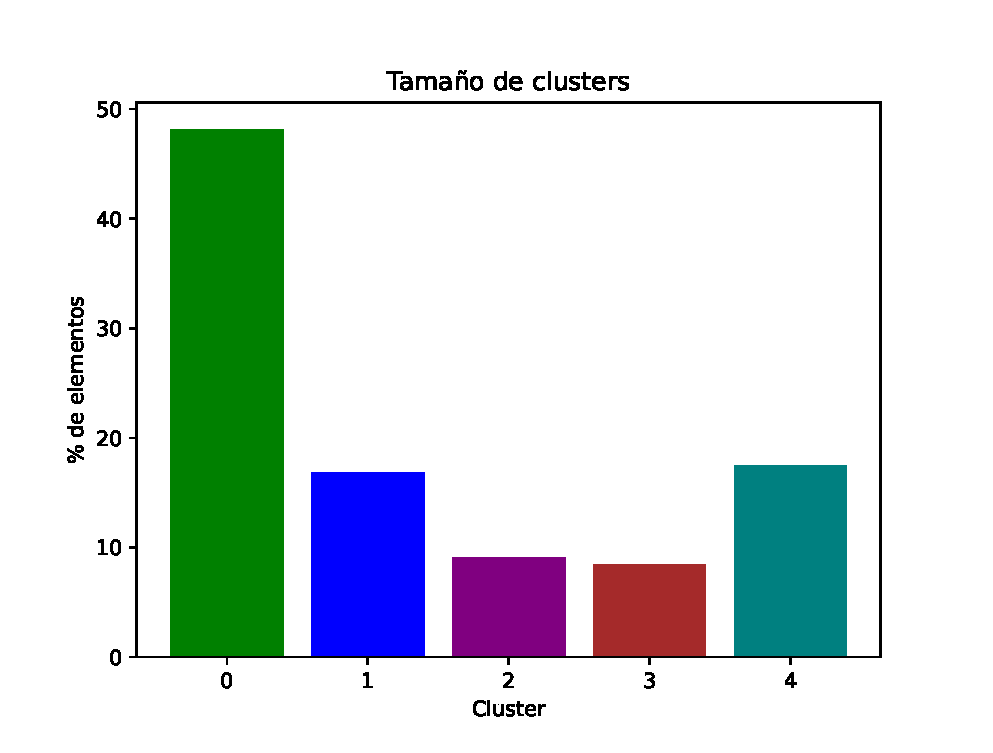
\includegraphics[scale=1]{caso1/spectral/bar.eps}
\end{figure}

A continuación observamos la scatter matrix \eqref{c1_scatter}, donde se puede apreciar como se separan los clusters y qué variables son necesarias para separar cada uno.

\begin{figure}[H]
\caption{Caso 1- Scatter matrix de spectral cluster}
\label{c1_scatter}
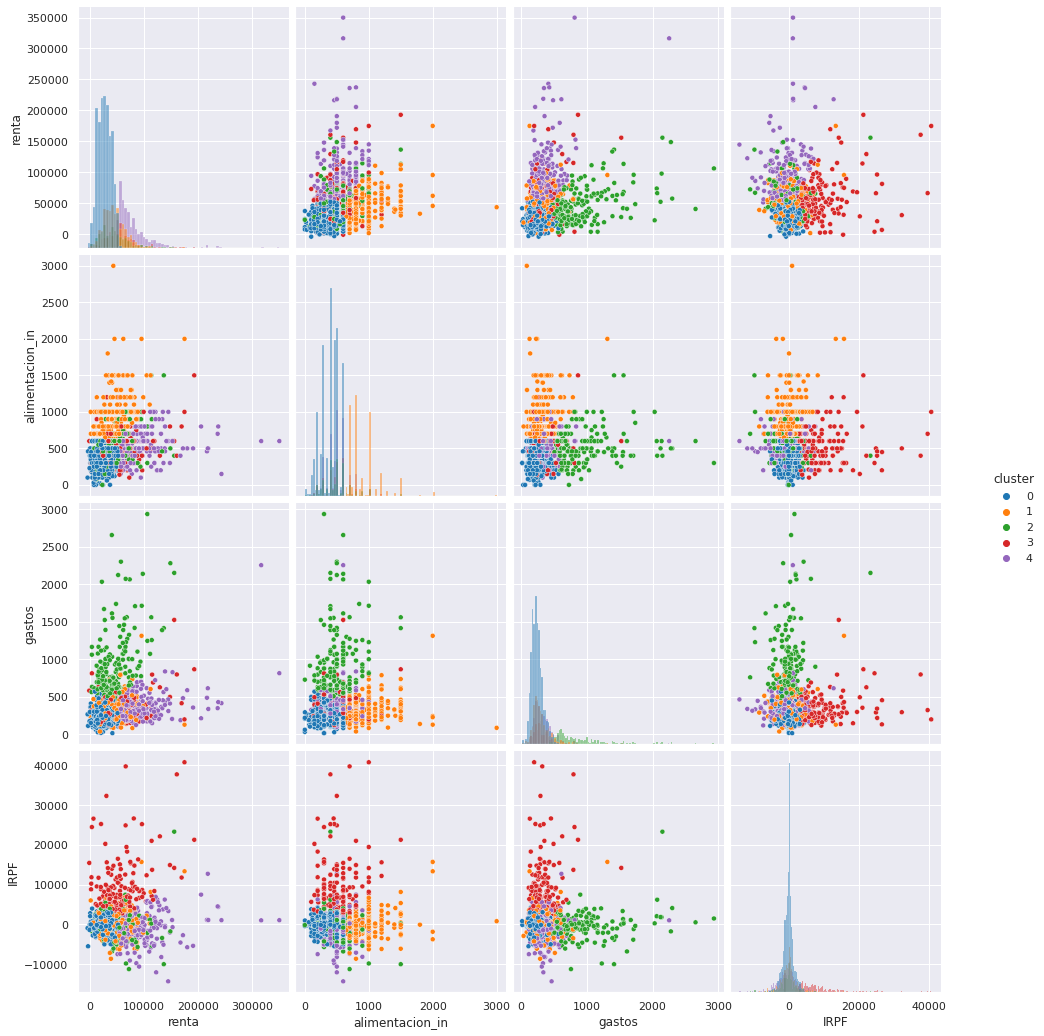
\includegraphics[scale=0.45]{caso1/spectral/scatter.png}
\end{figure}


\begin{figure}[H]
\caption{Caso 1- Boxplot de spectral cluster}
\label{c1_boxplot}
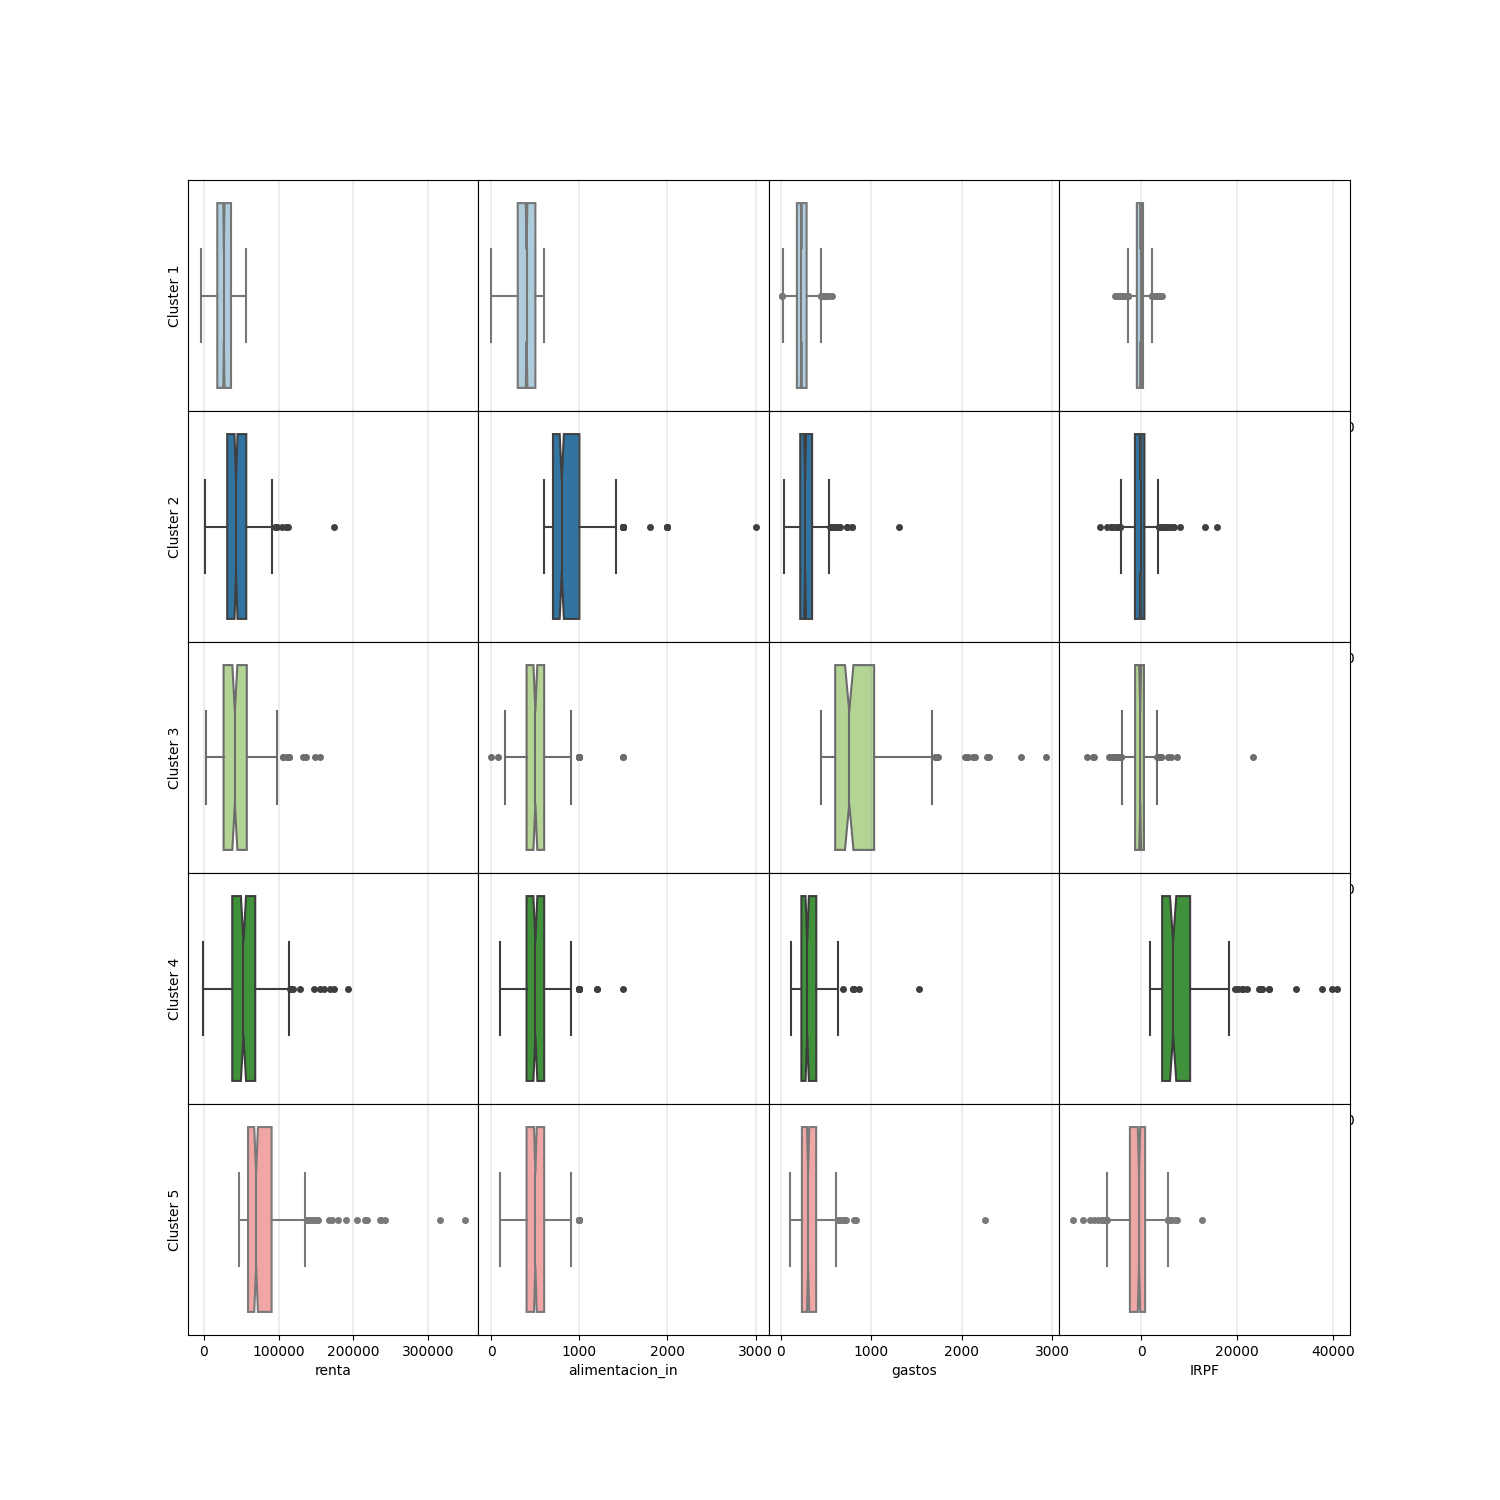
\includegraphics[scale=0.45]{caso1/spectral/boxplot.png}
\end{figure}

En \eqref{c1_boxplot} podemos observar como el cluster 3 toma valores en general mayores en gastos que los otros clusters. Esto también se observa en el cluster 4 con el IRPF y en el 2 con alimentacion in. Mientras los clusters 1 y 5 son más similares.

Notemos que al representar el boxplot la numeración de los clusters está de 1 a 5, mientras en la scatter matrix es de 0 a 4. Por tanto, hemos obtenido conclusiones análogas a las vistas en la scatter matrix.

\begin{figure}[H]
\caption{Caso 1- MDS de spectral cluster}
\label{c1_mds}
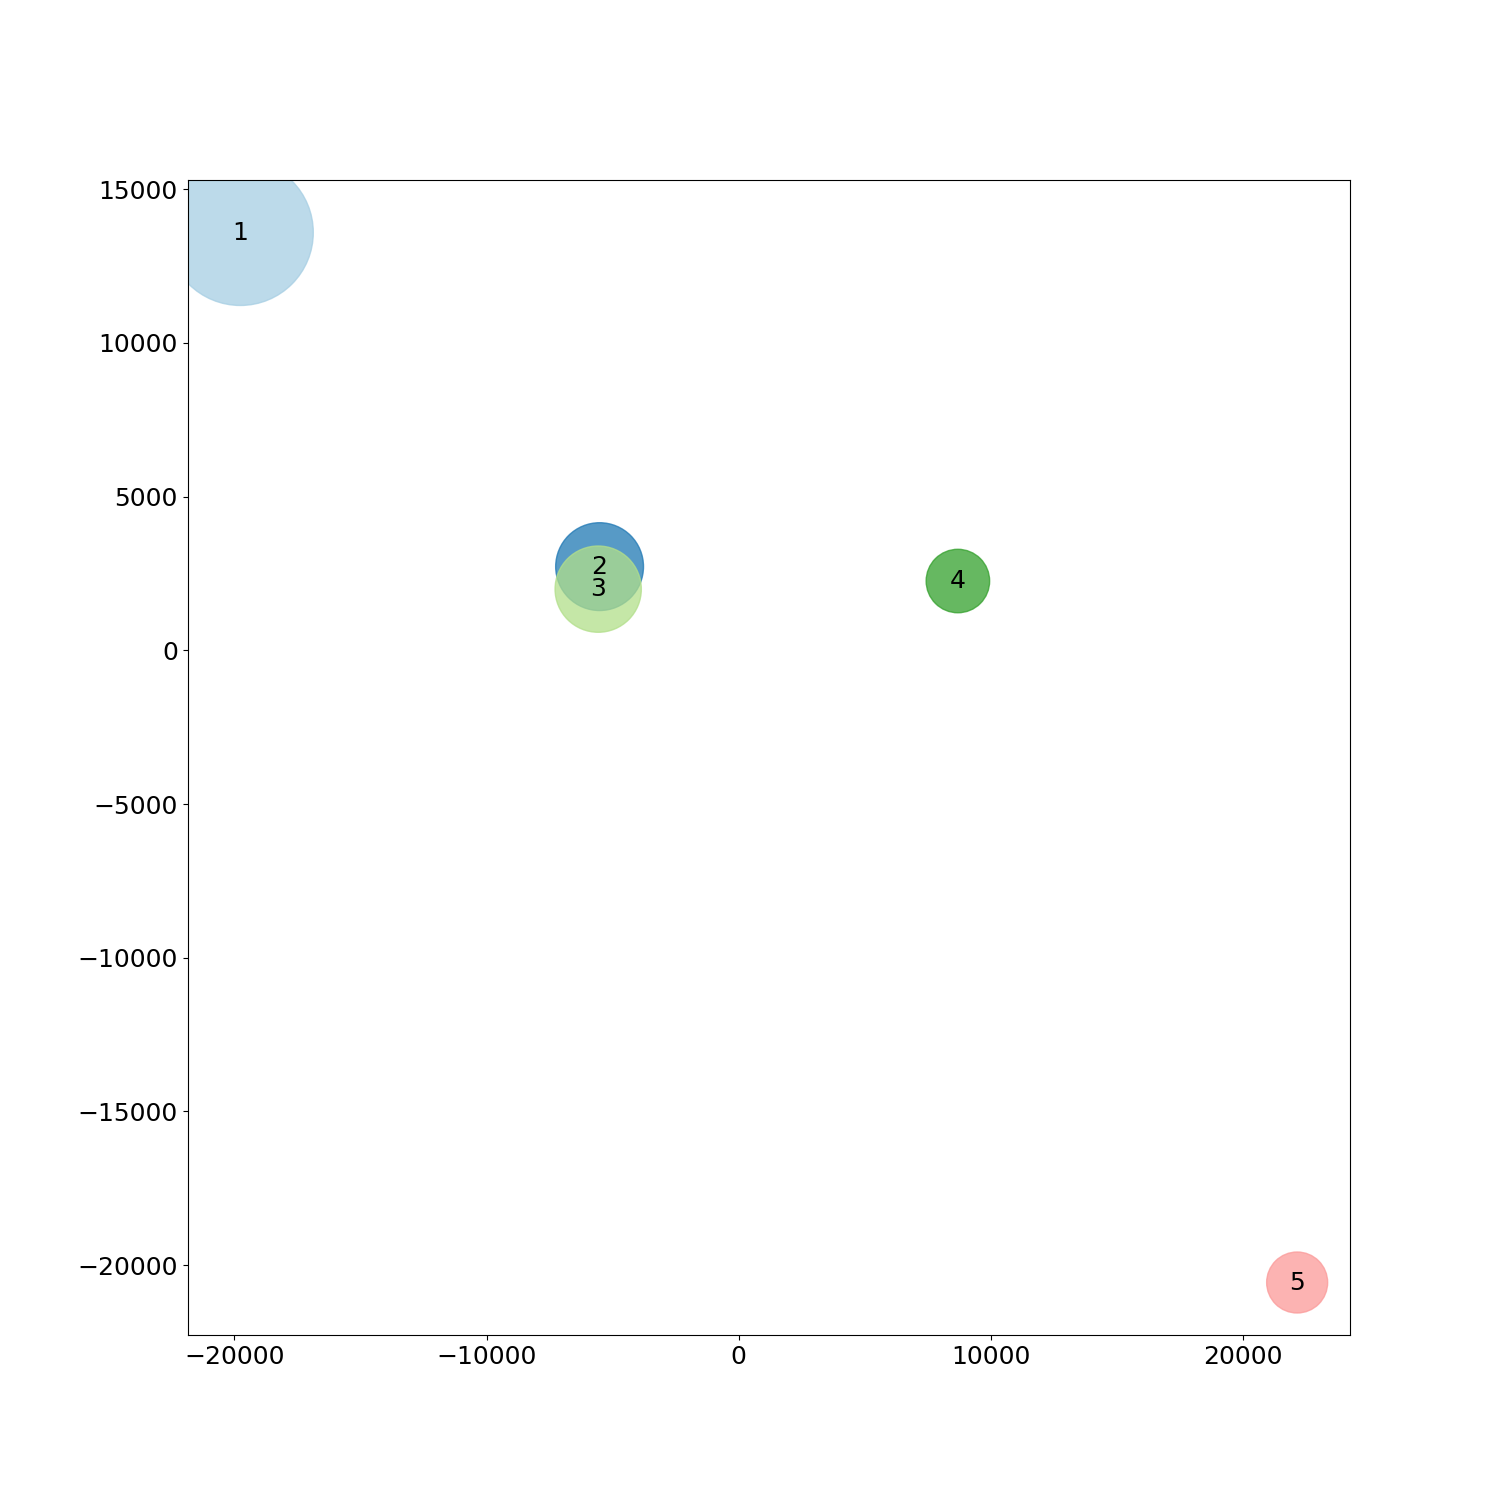
\includegraphics[scale=0.45]{caso1/spectral/mds.png}
\end{figure}

En \eqref{c1_mds} se aprecia como los clusters están considerablemente separados salvo dos que se superponen, aunque esto puede deberse a la proyección realizada. De nuevo, los clusters van de 1 a 5, pudiendo observarse desde otra perspectiva los tamaños de los clusters, cuyas proporciones coinciden con las expuestas anteriormente.


En la tabla  \eqref{tab:c1_variables} se muestran qué variables son necesarias para identificar cada cluster:

\begin{table}[H]
\centering
\caption{Caso 1 - Variables necesarias para separar el clustering en spectral cluster}
\label{tab:c1_variables}
\begin{tabular}{ccccc}
\toprule
 Cluster & renta & alimentacion in & gastos & IRPF \\
\midrule
0 & Baja & Baja & & \\
1 & & Alto & & \\
2 & & & Alto & \\
3 & & & & Alto \\
4 & Alta & Baja & & \\
\bottomrule
\end{tabular}
\end{table}
Como se aprecia en \eqref{tab:c1_variables} con una sola variable en cada cluster nos sirve para diferenciarlos entre ellos, mientras para los clusters 0 y 4 necesitamos dos para diferenciarlos entre ellos.

\section{Estudio de parámetros de DBSCAN}

Vamos a analizar el comportamiento de DBSCAN según sus parámetros principales. Para ello ejecutaremos la celda de parámetros de DBSCAN, que nos proporciona las medidas obtenidas para cada par de parámetros fijados.

\begin{table}
\centering
\caption{Caso 1 - Cambio de parámetros DBSCAN}
\label{tab:c1_dbscan}
\begin{tabular}{ccccccc}
\toprule
Algoritmo & eps & min samples & Tiempo(s) & Calinski-Harabasz & Silhouette & n clusters \\
\midrule
dbscan & 0.126 & 15 & 0.129 & 314.352 & 0.67749 & 2 \\
dbscan & 0.126 & 20 & 0.125 & 333.456 & 0.67367 & 2 \\
dbscan & 0.126 & 25 & 0.121 & 354.162 & 0.66902 & 2 \\
dbscan & 0.126 & 30 & 0.125 & 368.859 & 0.66260 & 2 \\
dbscan & 0.126 & 35 & 0.128 & 376.451 & 0.65698 & 2 \\
dbscan & 0.130 & 15 & 0.127 & 323.611 & 0.68333 & 2 \\
dbscan & 0.130 & 20 & 0.121 & 338.608 & 0.67757 & 2 \\
dbscan & 0.130 & 25 & 0.130 & 354.371 & 0.67411 & 2 \\
dbscan & 0.130 & 30 & 0.123 & 359.105 & 0.67258 & 2 \\
dbscan & 0.130 & 35 & 0.124 & 366.292 & 0.66568 & 2 \\
dbscan & 0.150 & 15 & 0.135 & 288.264 & 0.70224 & 2 \\
dbscan & 0.150 & 20 & 0.134 & 304.901 & 0.69936 & 2 \\
dbscan & 0.150 & 25 & 0.132 & 311.673 & 0.69243 & 2 \\
dbscan & 0.150 & 30 & 0.132 & 319.038 & 0.68550 & 2 \\
dbscan & 0.150 & 35 & 0.132 & 321.172 & 0.68152 & 2 \\
dbscan & 0.170 & 15 & 0.143 & 281.696 & 0.71489 & 2 \\
dbscan & 0.170 & 20 & 0.137 & 279.062 & 0.70922 & 2 \\
dbscan & 0.170 & 25 & 0.139 & 286.660 & 0.70839 & 2 \\
dbscan & 0.170 & 30 & 0.138 & 295.586 & 0.70562 & 2 \\
dbscan & 0.170 & 35 & 0.145 & 294.783 & 0.70345 & 2 \\
dbscan & 0.200 & 15 & 0.145 & 231.341 & 0.73756 & 2 \\
dbscan & 0.200 & 20 & 0.143 & 228.641 & 0.72741 & 2 \\
dbscan & 0.200 & 25 & 0.144 & 239.060 & 0.72724 & 2 \\
dbscan & 0.200 & 30 & 0.141 & 248.309 & 0.72676 & 2 \\
dbscan & 0.200 & 35 & 0.141 & 269.916 & 0.72272 & 2 \\
\bottomrule
\end{tabular}
\end{table}


Como podemos apreciar en \eqref{tab:c1_dbscan} DBSCAN siempre realiza dos clusters. El tamaño de estos es siempre similar, más del $90\%$ los ejemplos están agrupados en el cluster $0$ y los restantes están en el $-1$.

Este algoritmo no ha hecho ninguna buena agrupación en ningún caso de los probados, pese a que su silhouette es bastante alto, lo que puede ser consecuencia de que los clusters estén muy separados.

\begin{figure}[H]
\caption{Caso 1- Parámetros de DBSCAN}
\label{c1_param_dbscan}
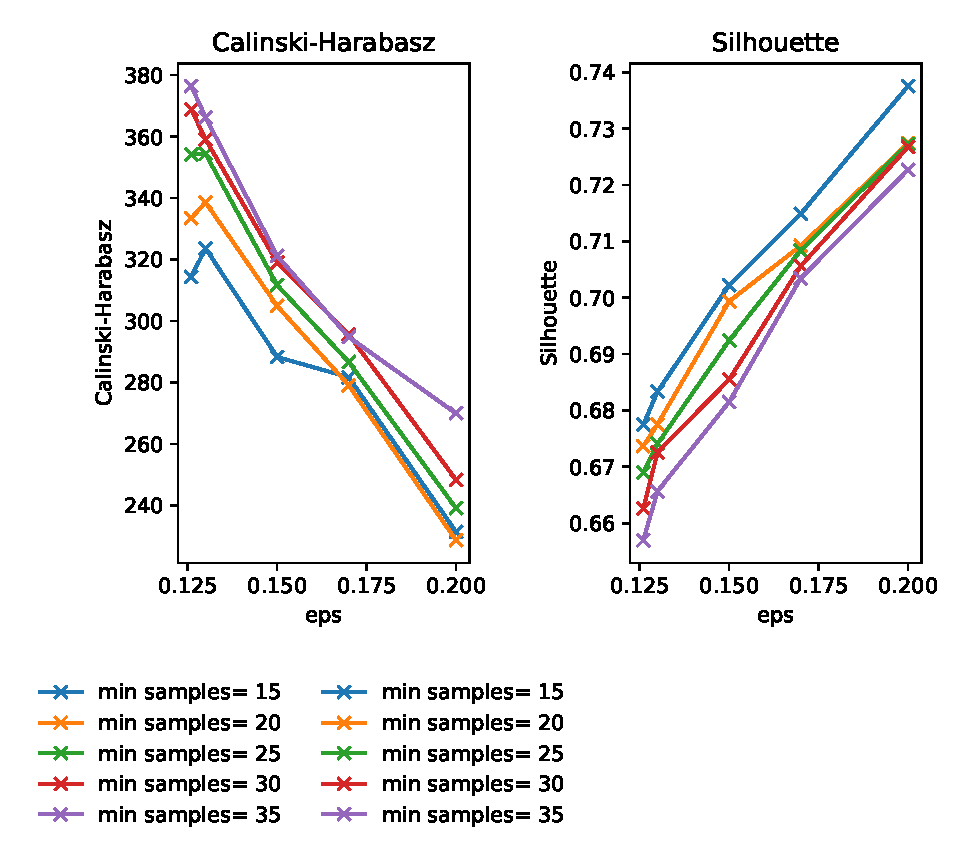
\includegraphics[scale=0.9]{caso1/parametros_dbscan.eps}
\end{figure}

No podemos interpretar demasiado Calinsk-Harabasz, ya que al no estar normalizado no sabemos si los valores dados son muy altos. Sí podemos decir que los mejores agrupamientos (que han proporcionado un valor de esta medida más alto) se han dado cuando min samples es $35$, como se puede ver en \eqref{c1_param_dbscan}.

También cabe destacar como el silhouette va creciendo conforme aumenta epsilon y calinski sube ligeramente al principio para valores bajos de min samples pero luego decrece, mientras para valores altos solo decrece. Asimismo resulta llamativo como los valores de min samples que producen valores de Calinski-harabasz más altos producen silhouettes más bajos.

Finalmente, cabe destacar como el tiempo de ejecución se incrementaba a la par que crecían los parámetros.


\section{Estudio de parámetros de Birch}

Estudiamos ahora el algoritmo Birch. Para este de nuevo se han probado distintas combinaciones de parámetros.

\begin{table}[H]
\centering
\caption{Caso 1 - Cambio de parámetros Birch}
\label{tab:c1_birch}
\begin{tabular}{ccccccc}
\toprule
Algoritmo & Branch fact & Threshold & Tiempo(s) & Calinski-Harabasz & Silhouette & n clusters \\
\midrule
birch & 15 & 0.100 & 0.087 & 336.711 & 0.48426 & 5 \\
birch & 15 & 0.150 & 0.065 & 192.073 & 0.58865 & 5 \\
birch & 15 & 0.200 & 0.060 & 206.873 & 0.60273 & 5 \\
birch & 15 & 0.250 & 0.062 &  &  & 1 \\
birch & 15 & 0.300 & 0.049 &  &  & 1 \\
birch & 20 & 0.100 & 0.147 & 173.266 & 0.58162 & 5 \\
birch & 20 & 0.150 & 0.077 & 180.842 & 0.58567 & 5 \\
birch & 20 & 0.200 & 0.046 & 206.873 & 0.60273 & 5 \\
birch & 20 & 0.250 & 0.053 &  &  & 1 \\
birch & 20 & 0.300 & 0.052 &  &  & 1 \\
birch & 25 & 0.100 & 0.153 & 312.603 & 0.49236 & 5 \\
birch & 25 & 0.150 & 0.064 & 184.304 & 0.57974 & 5 \\
birch & 25 & 0.200 & 0.045 & 206.873 & 0.60273 & 5 \\
birch & 25 & 0.250 & 0.051 &  &  & 1 \\
birch & 25 & 0.300 & 0.043 &  &  & 1 \\
birch & 30 & 0.100 & 0.136 & 292.036 & 0.52240 & 5 \\
birch & 30 & 0.150 & 0.059 & 184.304 & 0.57974 & 5 \\
birch & 30 & 0.200 & 0.066 & 206.873 & 0.60273 & 5 \\
birch & 30 & 0.250 & 0.057 &  &  & 1 \\
birch & 30 & 0.300 & 0.074 &  &  & 1 \\
birch & 35 & 0.100 & 0.129 & 355.783 & 0.42852 & 5 \\
birch & 35 & 0.150 & 0.058 & 184.304 & 0.57974 & 5 \\
birch & 35 & 0.200 & 0.061 & 206.873 & 0.60273 & 5 \\
birch & 35 & 0.250 & 0.061 &  &  & 1 \\
birch & 35 & 0.300 & 0.054 &  &  & 1 \\
\bottomrule
\end{tabular}
\end{table}

Podemos ver en \eqref{tab:c1_birch} como el algoritmo en general agrupa en $5$ clusters y obtiene resultados similares a kmeans. En general, ha hecho buenas agrupaciones a juzgar por las medidas.

Sin embargo, si miramos el tamaño de los clusters en muchas ocasiones estos se distriubuyen con un solo cluster agrupando el $90\%$ o más de los datos y los $4$ restantes el resto.

Cabe destacar que es bastante sensible a los parámetros, pues variando solo uno de ellos en ocasiones pasa de hacer 5 clusters a solo 1. Además, en estos casos no se proporcionan valores para las medidas Calinski-Harabasz y Silhouette, ya que para realizar estas es necesario tener más de un cluster.

\begin{figure}[H]
\caption{Caso 1- Parámetros de Birch}
\label{c1_param_birch}
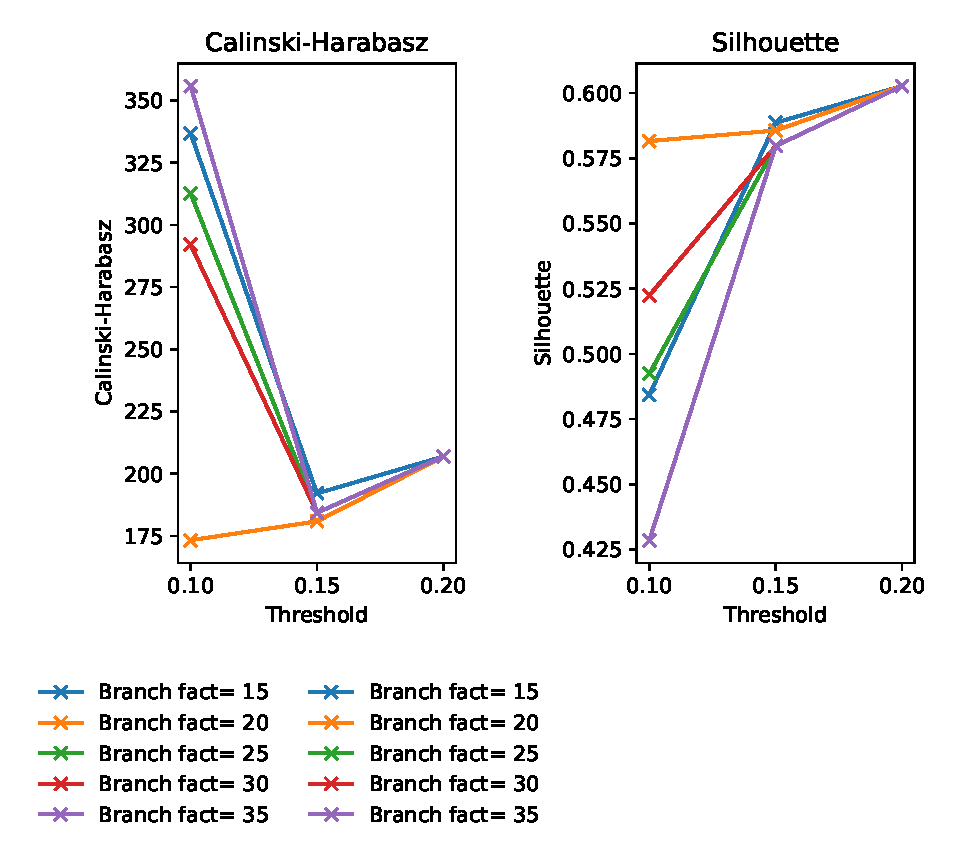
\includegraphics[scale=0.9]{caso1/parametros_birch.eps}
\end{figure}

En \eqref{c1_param_birch} se aprecia como para los valores de branch factor que producen mayor calinski-harabasz el silhouette es menor, y viceversa. Además, el silhouette siempre crece, mientras que Calinski-harabasz primero decrece y luego crece.

Teniendo en cuenta que Birch es una algoritmo que no está pensado para realizar clustering obteniendo todos los datos de una misma vez, ha generado un número de clusters razonable, pese a ser estas agrupaciones dudosas, pues los tamaños de estas son demasiado dispares.



\section{Interpretación de la segmentación}

A la vista de los resultados obtenidos, vemos que no se aprecian diferencias significativas en la renta entre las agrupaciones y no se encuentra demasiado dispersa. Esta variable por tanto no es tan relevante como otras.

No hay ninguna variable que destaque sobre otra, pero usando solamente las variables gastos, IRPF y alimentacion in podríamos diferenciar con claridad 3 clusters, y los otros dos agruparlos por descarte. Las otras variables nos sirvieron para refinar la diferenciación entre los clusters para lograr diferenciar los $5$.

Respecto a la hipótesis inicial, que las personas con propiedades alquiladas tienen mayor renta y por tanto más comodidades, en principio no parece cierta, pues la renta no ha sido una variable significativa respecto a la que dividir y otros factores son más influyentes.





%\ctparttext{\color{black}\begin{center}
%		Esta es una descripción de la parte de informática.
%\end{center}}

%\part{Parte de informática}
\chapter{Caso 2: Comparación de rentas}


\section{Descripción del caso de estudio}
Este caso de estudio trata de contrastar las diferencias que hay entre grupos con renta baja (menor de $15000$€ al año) y renta alta (mayor de $25000$€ al año).

Para ello, las variables seleccionas son:
\begin{itemize}
\item \textbf{Renta}: Renta disponible total del hogar en el año anterior al de encuesta.
\item \textbf{Alimentos}: Durante el mes pasado, ¿cuál fue aproximadamente el importe que el hogar gastó en alimentos y bebidas no alcohólicas para ser consumidas en casa?
\item \textbf{Asistencia social}: Ingresos por asistencia social en el año anterior al
de encuesta.
\item \textbf{Gastos}: Gastos de la vivienda: Alquiler (si la vivienda se encuentra en régimen de alquiler), intereses de la hipoteca (para viviendas en propiedad con pagos pendientes) y otros gastos asociados (comunidad, agua, electricidad, gas, etc.)
\end{itemize}

Para realizar la comparativa, vamos a estudiar dos subcasos, el primero con renta baja y el segundo con renta alta.

\section{Caso 2 A: Renta baja}

Este caso de estudio consta de $3197$ elementos, cada uno con las cuatro variables especificadas antes.

\subsection{Ejecución de algoritmos}

Ejecutamos la celda del notebook de jupyter correspondiente al caso 2A (que se puede configurar para sacar las distintas gráficas) y obtenemos así las diferentes medidas obtenidas para cada algoritmo, que se muestran en \eqref{tab:c2A_alg}.

\begin{table}[H]
\centering
\caption{Caso 2A - Resultados de ejecución de algoritmos.}
\label{tab:c2_alg}
\begin{tabular}{ccccc}
\toprule
 Algoritmo & Tiempo (s) & Silhouette & Calinski-Harabasz & Número de clusters \\
\midrule
kmeans & 0.385 & 1157.588 & 0.31325 & 5 \\
birch & 0.124 & 510.565 & 0.26449 & 5 \\
spectral & 1.739 & 1068.474 & 0.30286 & 5 \\
dbscan & 0.171 & 304.282 & 0.60850 & 2 \\
meanshift & 18.233 & 184.067 & 0.40807 & 11 \\
\bottomrule
\end{tabular}
\end{table}

Respecto a los tiempos, de nuevo el algoritmo más lento es meanshift, seguido de spectral cluster. El resto de algoritmos obtienen tiempo similares.

Además, al igual que en el caso 1 DBSCAN ha generado solamente dos clusters, uno con el $97.12\%$ de los datos y los restantes en el cluster -1.Meanshift vuelve a generar más cluster que el resto, agrupanod uno de ellos al $91.46\%$ de elementos, otro al $4.86\%$ y el resto cada uno contiene un número de elementos menor al $1.2\%$ del total. Por ello, parece que a pesar de las medidas que han obtenido, estos algoritmos no han realizado un buen agrupamiento.

Finalmente vemos como Birch tiene un valor de Calinski-Harabasz y silhouette más bajo que kmeans y spectral cluster. Estos algoritmos han conseguido medidas similares, obteniendo en principio kmeans mejores resultados.


\subsection{Análisis}


Para el análisis se va a usar kmeans, ya que ha obtenido los mejores en las medidas. Este algoritmo genera 5 clusters. Se ha generado un cluster de tamaño menor, y los otros tienen tamaños similares dos a dos, como se puede ver en \eqref{c2A_tam}.

\begin{figure}[H]
\caption{Caso 2A- Tamaño de los clusters generados por kmeans}
\label{c2A_tam}
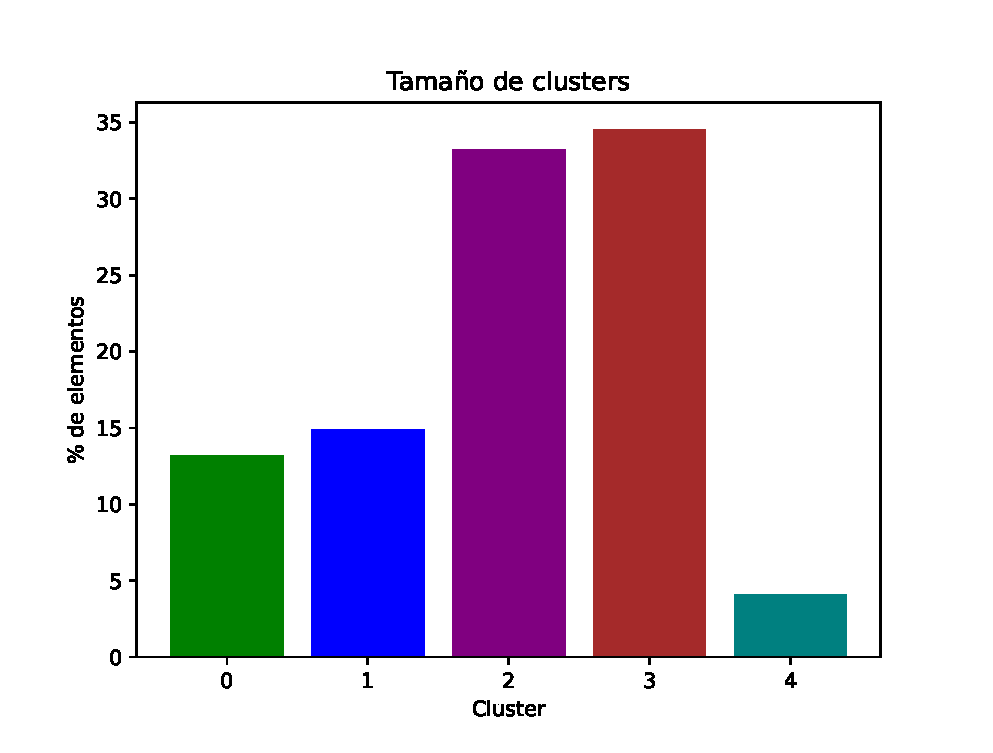
\includegraphics[scale=1]{caso2A/kmeans/bar.eps}
\end{figure}

A continuación observamos la scatter matrix \eqref{c2A_scatter}, donde se puede apreciar como se separan os clusters y qué variables son necesarias para separar cada uno. Hay varios clusters que se diferencian bien con una sola variable, como es el caso de cluster 0, que tiene valores altos de gastos, el 4 tiene valores más altos en asistencia social y el 2 gasta más en alimentación. Los clusters 1 y 3 se distinguen bien usando renta y gastos o renta y alimentos, ya que ambos tienen valores bajos de renta y uno tiene valores mayores que el otro en la variable restante.

\begin{figure}[H]
\caption{Caso 2A- Scatter matrix de kmeans}
\label{c2A_scatter}
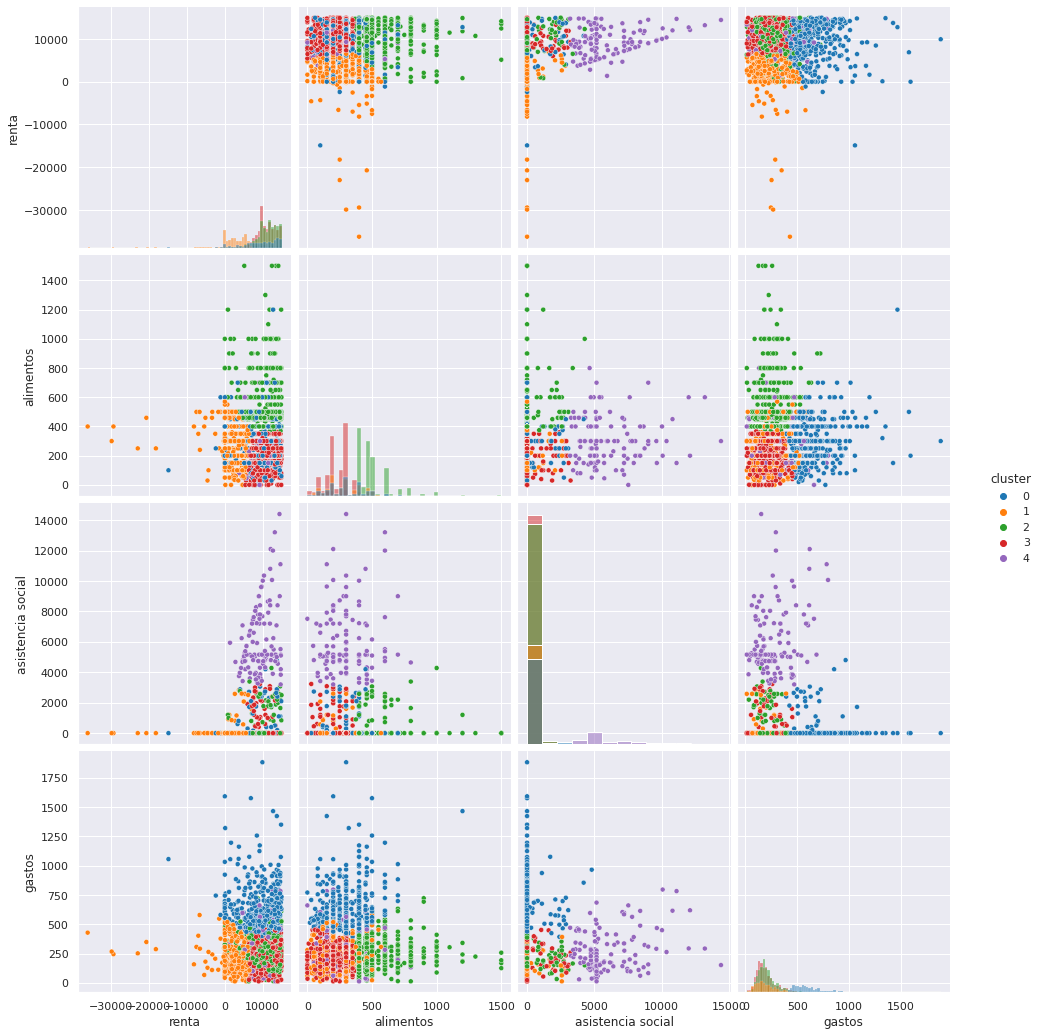
\includegraphics[scale=0.45]{caso2A/kmeans/scatter.png}
\end{figure}


\begin{figure}[H]
\caption{Caso 2A- Heatmap de kmeans}
\label{c2A_heatmap}
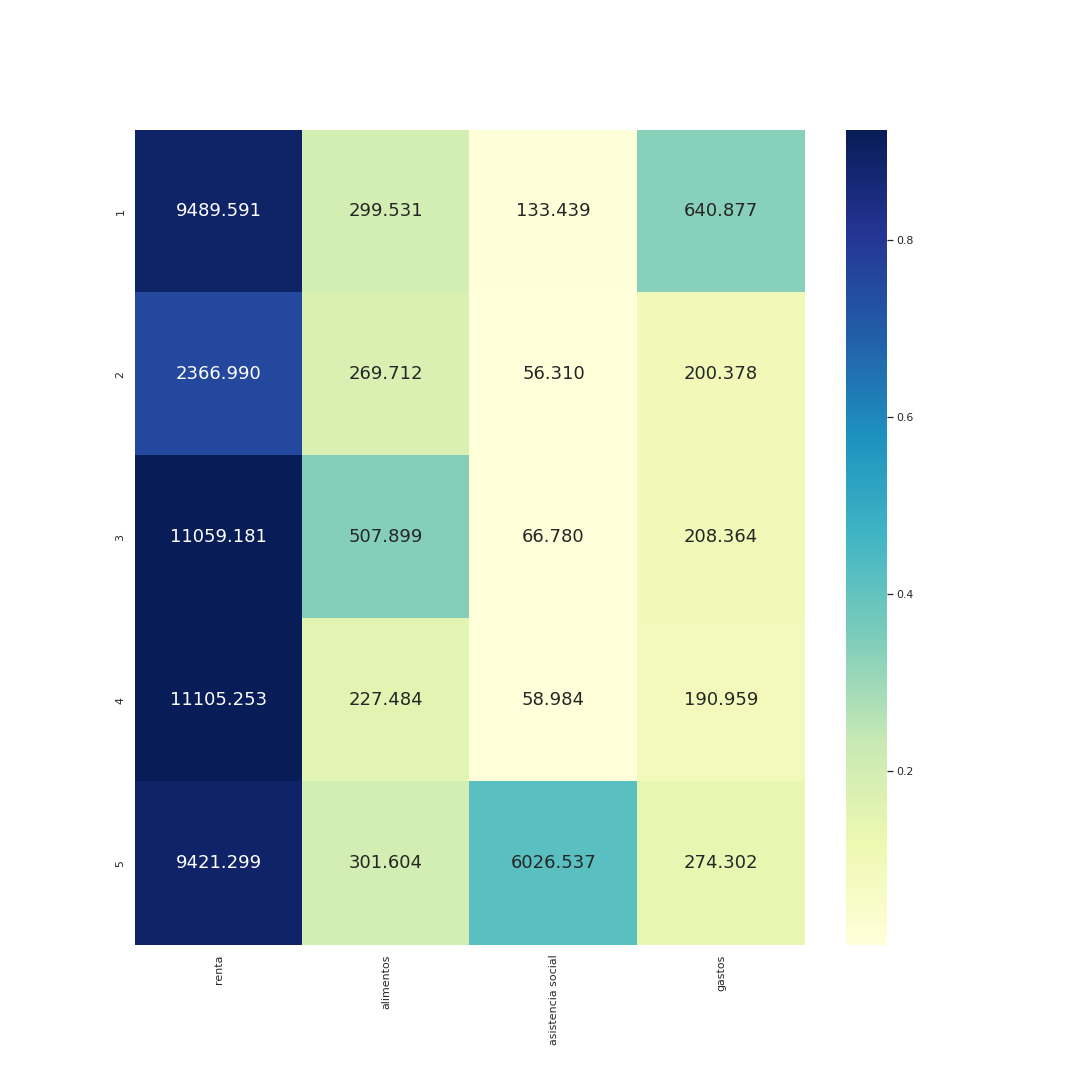
\includegraphics[scale=0.45]{caso2A/kmeans/heatmap.png}
\end{figure}

En \eqref{c2A_heatmap} se ve con claridad los tres clusters que se diferencian por tomar valores especialmente altos en una de sus variables. Teniendo en cuenta que la numeración en este gráfico va de 1 a 5 y en la scatter matrix va de 0 a 4, vemos la analogía. En el heatmap se ve con claridad como el cluster 5 toma valores considerablemente más altos en asistencia social que el resto de clusters, el 3 toma valores más altos en alimentación y el 1 en gastos, lo que concuerda con lo visto en la scatter matrix.


\begin{figure}[H]
\caption{Caso 2A- MDS de kmeans}
\label{c2A_mds}
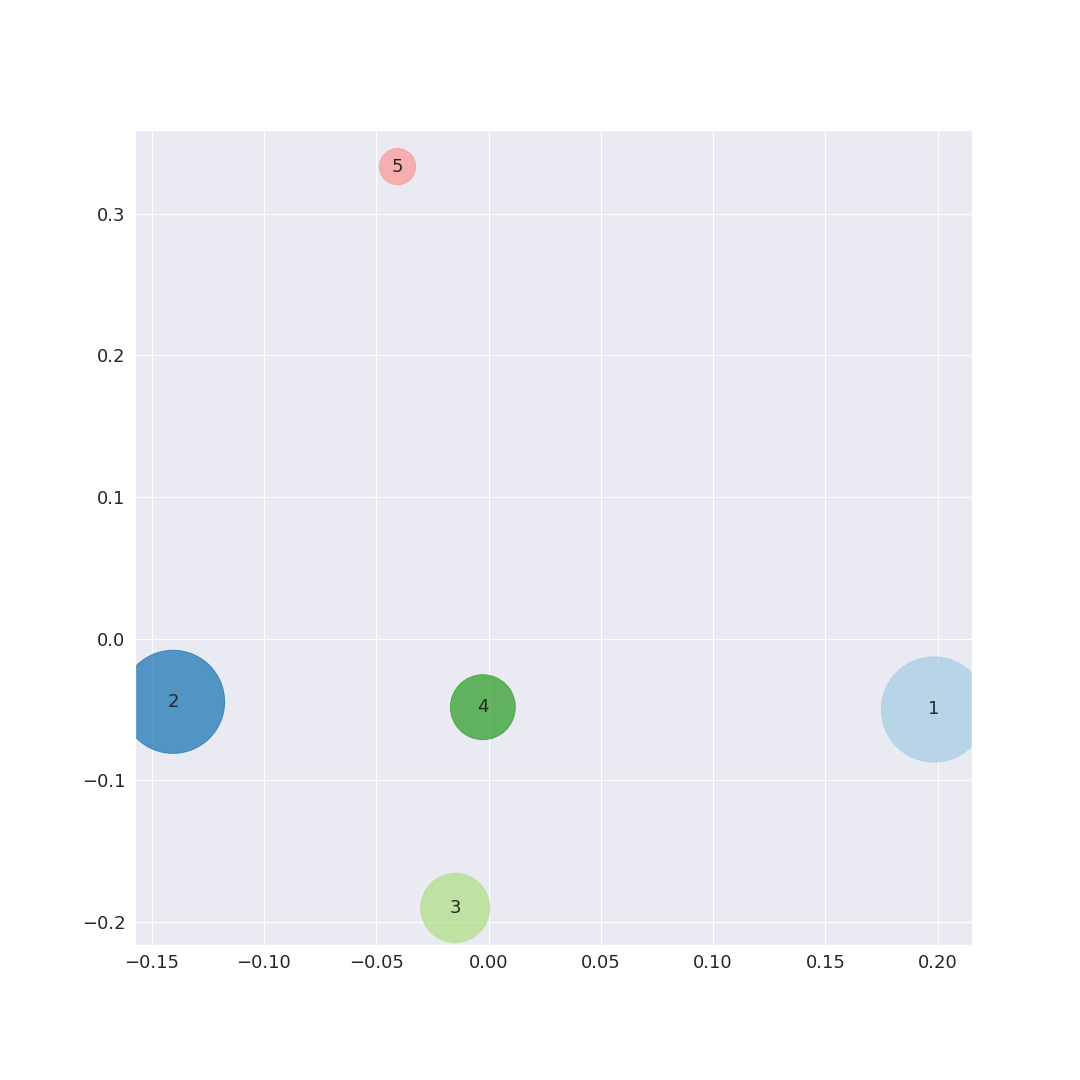
\includegraphics[scale=0.45]{caso2A/kmeans/mds.png}
\end{figure}

En \eqref{c2A_mds} se aprecia como los clusters están separados entre sí y tienen tamaños similares salvo por elc luster 5, que es de menor tamaño.

\begin{figure}[H]
\caption{Caso 2A - Parallel coordinates de kmeans}
\label{c2A_parallel}
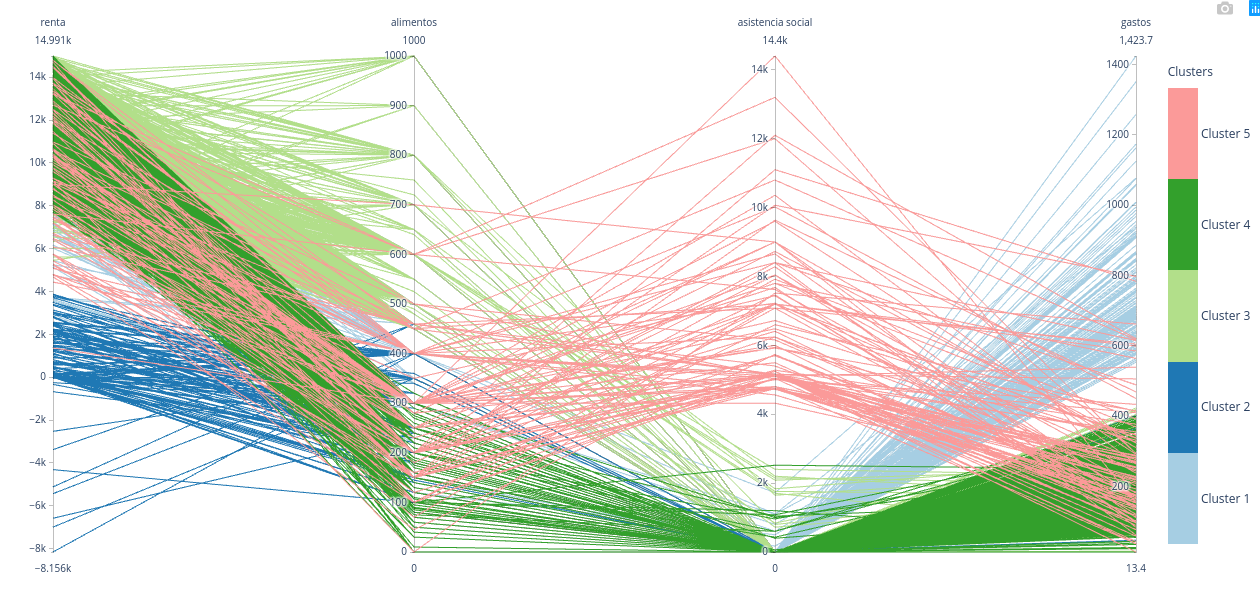
\includegraphics[scale=0.4]{caso2A/kmeans/parallel.png}
\end{figure}

En \eqref{c2A_parallel} se aprecia como el cluster verde claro, que alcanza mayores valores de asistencia social, es más disperso que los demás, lo que concuerda con la scatter matrix \eqref{c2A_scatter}. De nuevo, es claro que hay dos clusters que se diferencian por sus valores altos en alimentación y gastos.

En la tabla  \eqref{tab:c2A_variables} se muestran qué variables son necesarias para identificar cada cluster:

\begin{table}[H]
\centering
\caption{Caso 2A - Variables necesarias para separar el clustering en spectral cluster}
\label{tab:c2A_variables}
\begin{tabular}{ccccc}
\toprule
 Cluster & renta & alimentos & asistencia social & gastos \\
\midrule
0 & & & & X \\
1 & X & & & X \\
2 & & X & & \\
3 & X & & & X \\
4 & & & X & \\
\bottomrule
\end{tabular}
\end{table}
Como se aprecia en \eqref{tab:c2A_variables} con una sola variable en cada cluster nos sirve para diferenciarlos entre los clusters 0, 2 y 4, mientras para los clusters 1 y 3 necesitamos dos para diferenciarlos entre ellos.

\subsection{Estudio de parámetros de DBSCAN}

Vamos a analizar el comportamiento de DBSCAN según sus parámetros principales. Para ello ejecutaremos la celda de parámetros de DBSCAN, que nos proporciona las medidas obtenidas para cada par de parámetros fijados.

\begin{table}[H]
\centering
\caption{Caso 2A - Cambio de parámetros DBSCAN}
\label{tab:c2A_dbscan}
\begin{tabular}{ccccccc}
\toprule
 Algoritmo & Tiempo (s) & Silhouette & Calinski-Harabasz & Número de clusters \\
\midrule
dbscan & 0.126 & 15.000 & 0.210 & 283.280 & 0.62692 & 2 \\
dbscan & 0.126 & 20.000 & 0.177 & 304.282 & 0.60850 & 2 \\
dbscan & 0.126 & 25.000 & 0.185 & 343.349 & 0.59182 & 2 \\
dbscan & 0.126 & 30.000 & 0.181 & 357.820 & 0.58212 & 2 \\
dbscan & 0.126 & 35.000 & 0.188 & 361.064 & 0.57576 & 2 \\
dbscan & 0.130 & 15.000 & 0.190 & 223.006 & 0.63128 & 2 \\
dbscan & 0.130 & 20.000 & 0.194 & 279.313 & 0.62217 & 2 \\
dbscan & 0.130 & 25.000 & 0.184 & 324.483 & 0.60954 & 2 \\
dbscan & 0.130 & 30.000 & 0.193 & 345.157 & 0.60186 & 2 \\
dbscan & 0.130 & 35.000 & 0.193 & 354.160 & 0.58156 & 2 \\
dbscan & 0.150 & 15.000 & 0.247 & 133.391 & 0.67010 & 2 \\
dbscan & 0.150 & 20.000 & 0.212 & 208.220 & 0.65089 & 2 \\
dbscan & 0.150 & 25.000 & 0.213 & 234.186 & 0.64523 & 2 \\
dbscan & 0.150 & 30.000 & 0.219 & 244.053 & 0.63871 & 2 \\
dbscan & 0.150 & 35.000 & 0.232 & 277.293 & 0.63108 & 2 \\
dbscan & 0.170 & 15.000 & 0.245 & 106.562 & 0.68737 & 2 \\
dbscan & 0.170 & 20.000 & 0.243 & 112.836 & 0.68127 & 2 \\
dbscan & 0.170 & 25.000 & 0.241 & 154.421 & 0.66746 & 2 \\
dbscan & 0.170 & 30.000 & 0.231 & 179.415 & 0.66353 & 2 \\
dbscan & 0.170 & 35.000 & 0.479 & 197.375 & 0.66118 & 2 \\
dbscan & 0.200 & 15.000 & 0.283 & 77.501 & 0.69224 & 2 \\
dbscan & 0.200 & 20.000 & 0.256 & 95.258 & 0.68918 & 2 \\
dbscan & 0.200 & 25.000 & 0.254 & 103.127 & 0.68949 & 2 \\
dbscan & 0.200 & 30.000 & 0.252 & 107.818 & 0.68620 & 2 \\
dbscan & 0.200 & 35.000 & 0.239 & 110.824 & 0.68431 & 2 \\
\bottomrule
\end{tabular}
\end{table}

Como podemos apreciar en \eqref{tab:c2A_dbscan} DBSCAN siempre realiza dos clusters. El tamaño de estos es siempre similar, más del $90\%$ los ejemplos están agrupados en el cluster $0$ y los restantes están en el $-1$.

Este algoritmo no ha hecho ninguna buena agrupación en ningún caso de los probados, pese a que su silhouette es bastante alto, lo que puede ser consecuencia de que los clusters estén muy separados.

No podemos interpretar demasiado Calinsk-Harabasz, ya que al no estar normalizado no sabemos si los valores dados son muy altos. Sí podemos decir que los mejores agrupamientos (que han proporcionado un valor de esta medida más alto) se han dado cuando min samples es $15$.


\subsection{Estudio de parámetros de Kmeans}

Estudiamos ahora el algoritmo Kmeans. Se ha variado el número de clusters.

\begin{table}[H]
\centering
\caption{Caso 2A - Cambio de parámetros Kmeans}
\label{tab:c2A_kmeans}
\begin{tabular}{cccccc}
\toprule
Algoritmo & n clusters & Tiempo(s) & Silhouette & Calinski-Harabasz & n clusters \\
\midrule
kmeans & 3.000 & 0.224 & 960.927 & 0.28417 & 3 \\
kmeans & 4.000 & 0.122 & 1162.049 & 0.31899 & 4 \\
kmeans & 5.000 & 0.283 & 1157.588 & 0.31325 & 5 \\
kmeans & 6.000 & 0.292 & 1174.483 & 0.32302 & 6 \\
kmeans & 7.000 & 0.328 & 1107.187 & 0.31675 & 7 \\
kmeans & 8.000 & 0.183 & 1074.974 & 0.31710 & 8 \\
kmeans & 9.000 & 0.487 & 1031.378 & 0.31904 & 9 \\
kmeans & 10.000 & 1.043 & 992.485 & 0.29012 & 10 \\
\bottomrule
\end{tabular}
\end{table}

Podemos ver en \eqref{tab:c2A_kmeans} que no hay demasiada diferencia entre las medidas obtenidas para los distintos valores del número de clusters, y destaca que el valor para el que se alcanza el máximo en Silhouette es el mismo para el que se alcanza el máximo en Calinski-harabasz, que es 6 clusters.

Aún así, kmeans ha dado resultados buenos en todos los casos y ha demostrado ser bastante robusto en sus agrupaciones.



\section{Caso 2 B: Renta alta}

Este caso de estudio consta de $8372$ elementos, cada uno con las cuatro variables especificadas antes.

\subsection{Ejecución de algoritmos}

Ejecutamos la celda del notebook de jupyter correspondiente al caso 2B y obtenemos las diferentes medidas obtenidas para cada algoritmo, que se muestran en \eqref{tab:c2B_alg}.

\begin{table}[H]
\centering
\caption{Caso 2B - Resultados de ejecución de algoritmos.}
\label{tab:c2_alg}
\begin{tabular}{ccccc}
\toprule
 Algoritmo & Tiempo (s) & Silhouette & Calinski-Harabasz & Número de clusters \\
\midrule
kmeans & 0.531 & 2962.319 & 0.30911 & 5 \\
birch & 0.312 & 645.084 & 0.47807 & 5 \\
spectral & 20.642 & 2145.100 & 0.32184 & 5 \\
dbscan & 1.532 & 473.629 & 0.75774 & 2 \\
meanshift & 68.273 & 211.786 & 0.40726 & 31 \\
\bottomrule
\end{tabular}
\end{table}

Respecto a los tiempos, de nuevo el algoritmo más lento es meanshift, seguido de spectral cluster. El resto de algoritmos obtienen tiempo similares. Cabe destacar que al incrementarse el número de instancias los tiempo han subido considerablemente, en especial el de meanshift, ya que calcular bandwith es costoso.

Además, al igual que en los casos anteriores DBSCAN ha generado solamente dos clusters, uno con el $99.44\%$ de los datos y los restantes en el cluster -1. Meanshift vuelve a generar más cluster que el resto, agrupando uno de ellos el $93.37\%$ de elementos, y el resto son  agrupaciones de menos el $2\%$ de elementos. Por ello, parece que a pesar de las medidas que han obtenido, estos algoritmos no han realizado un buen agrupamiento.

Finalmente vemos como Birch tiene un valor de Calinski-Harabasz más bajo que kmeans y spectral cluster, aunque obtiene un silhouette mayor.

\subsection{Análisis}


Para el análisis se va a usar kmeans, como se hizo en el caso anterior para poder realizar la comparación. Este algoritmo genera 5 clusters. Se ha generado un cluster grande con algo más e la mitad de los datos, uno mediano y el resto pequeños, como se puede ver en \eqref{c2B_tam}.

\begin{figure}[H]
\caption{Caso 2B- Tamaño de los clusters generados por kmeans}
\label{c2B_tam}
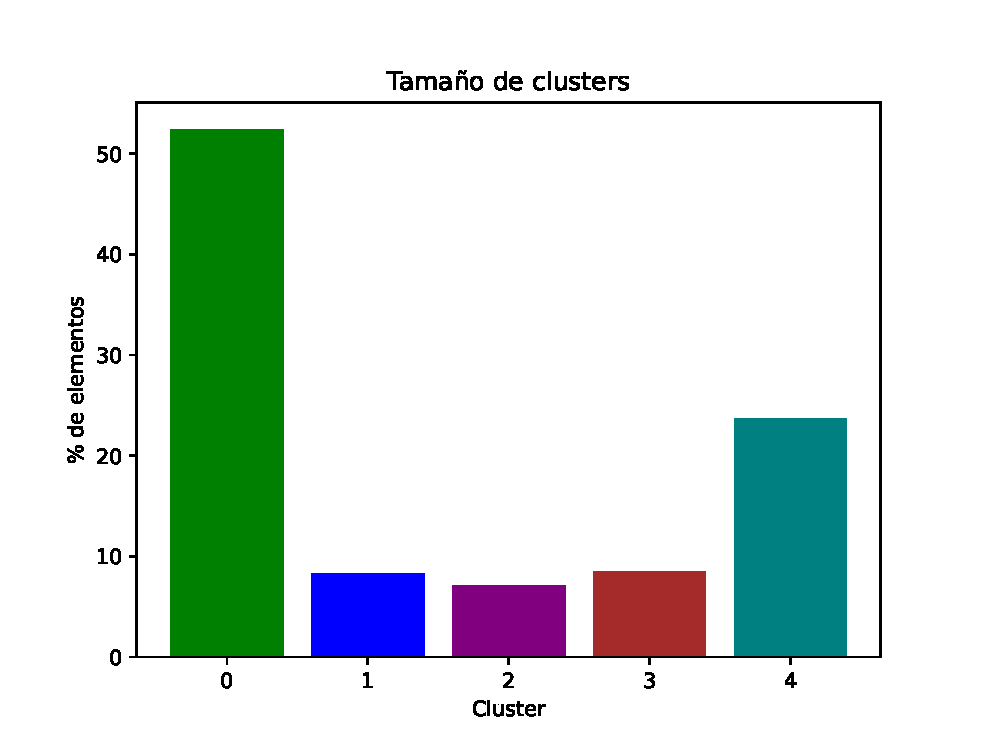
\includegraphics[scale=1]{caso2B/kmeans/bar.eps}
\end{figure}

A continuación observamos la scatter matrix \eqref{c2B_scatter}, donde se puede apreciar como se separan os clusters y qué variables son necesarias para separar cada uno. De manera análoga al caso 2A vemos como se pueden separar varios clusters solamente por valores altos de ciertas variables, que son el cluster 1 con grandes gastos, el 2 con alimentos y el 3 por valores muy altos de renta. Los clusters 0 y 4 requieren de varias variables para distinguirse, que son alimentos y gastos.

\begin{figure}[H]
\caption{Caso 2B- Scatter matrix de kmeans}
\label{c2B_scatter}
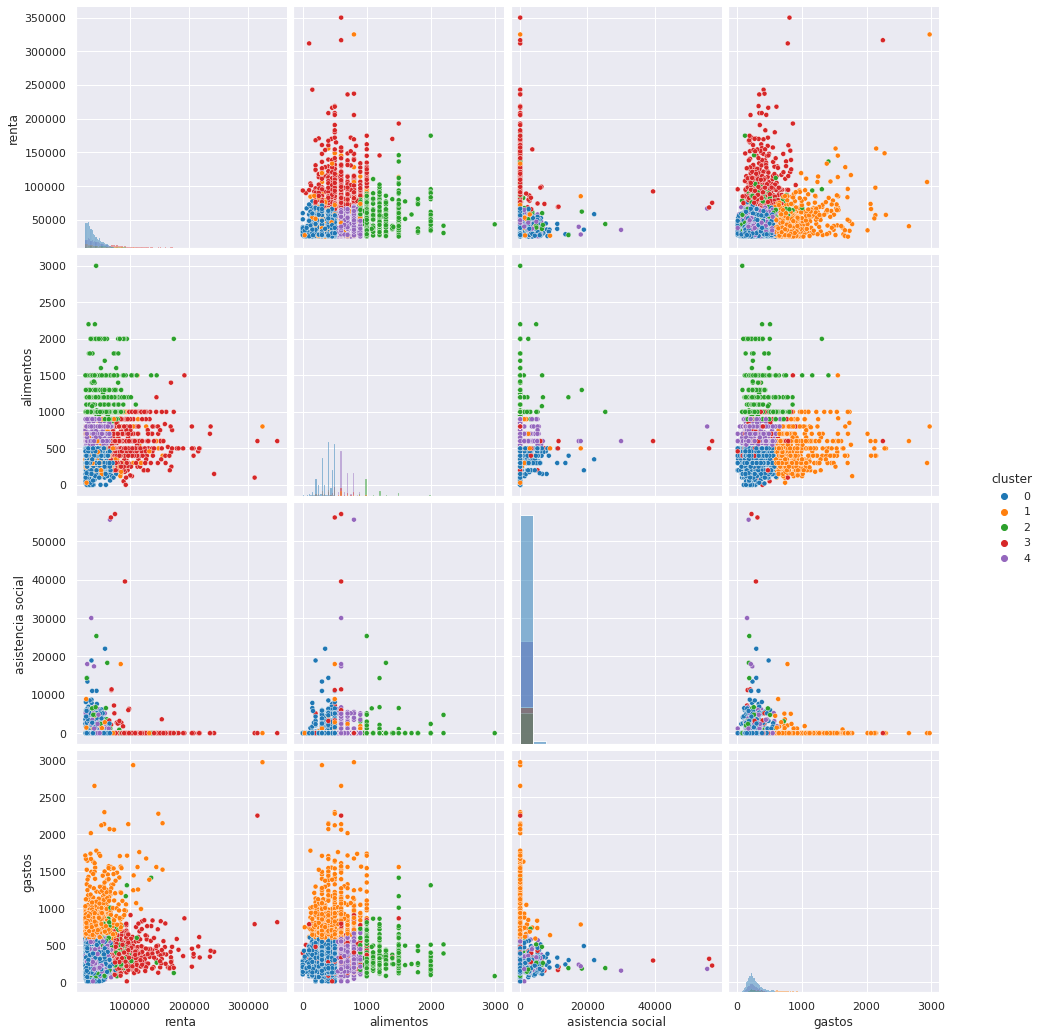
\includegraphics[scale=0.45]{caso2B/kmeans/scatter.png}
\end{figure}


\begin{figure}[H]
\caption{Caso 2B- Heatmap de kmeans}
\label{c2B_heatmap}
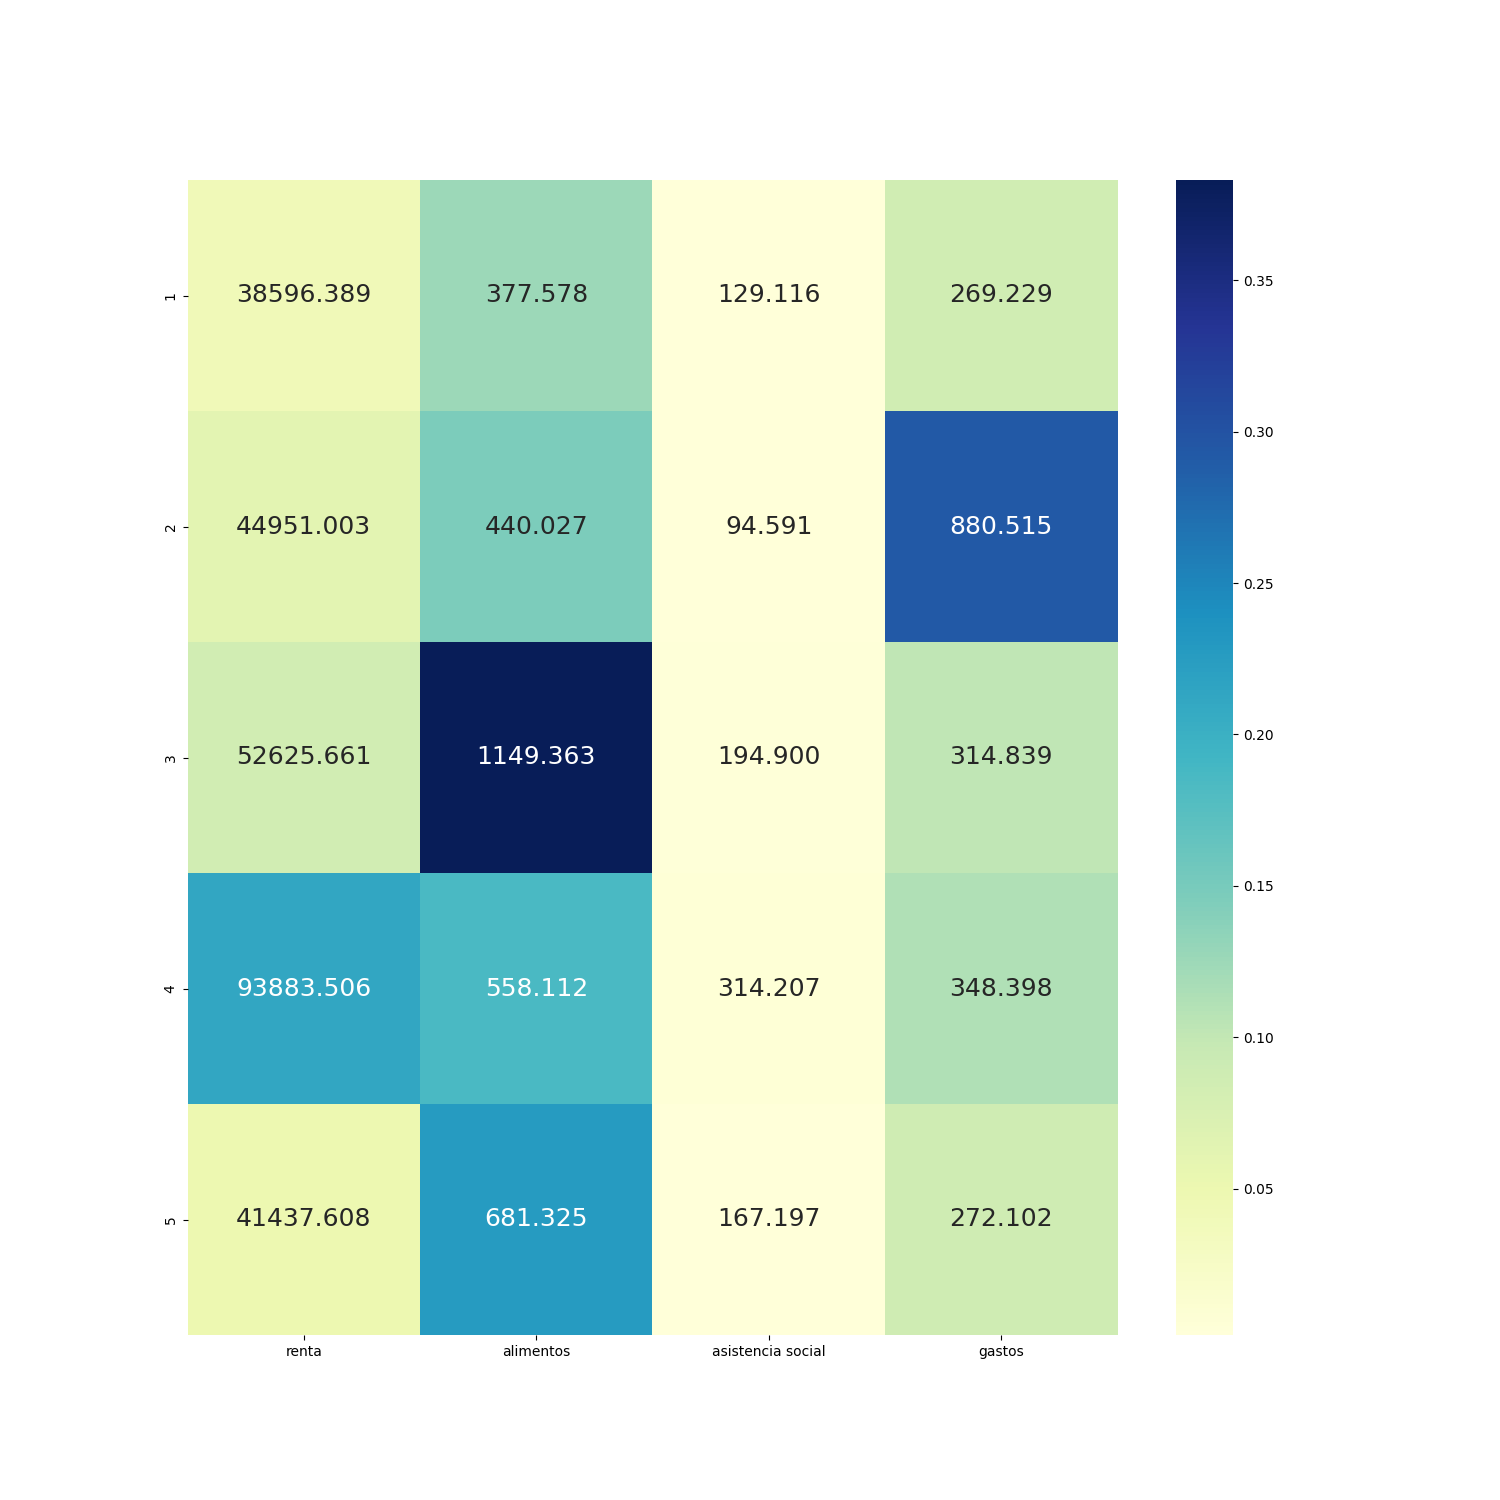
\includegraphics[scale=0.45]{caso2B/kmeans/heatmap.png}
\end{figure}

En \eqref{c2B_heatmap} se ve con claridad los tres clusters que se diferencian por tomar valores especialmente altos en una de sus variables. Teniendo en cuenta que la numeración en este gráfico va de 1 a 5 y en la scatter matrix va de 0 a 4, vemos la analogía. En el heatmap se distingue como el cluster 2 toma valores considerablemente más altos en gastos que el resto de clusters, el 3 toma valores más altos en alimentación y el 4 en renta, lo que concuerda con lo visto en la scatter matrix.


\begin{figure}[H]
\caption{Caso 2B- MDS de kmeans}
\label{c2B_mds}
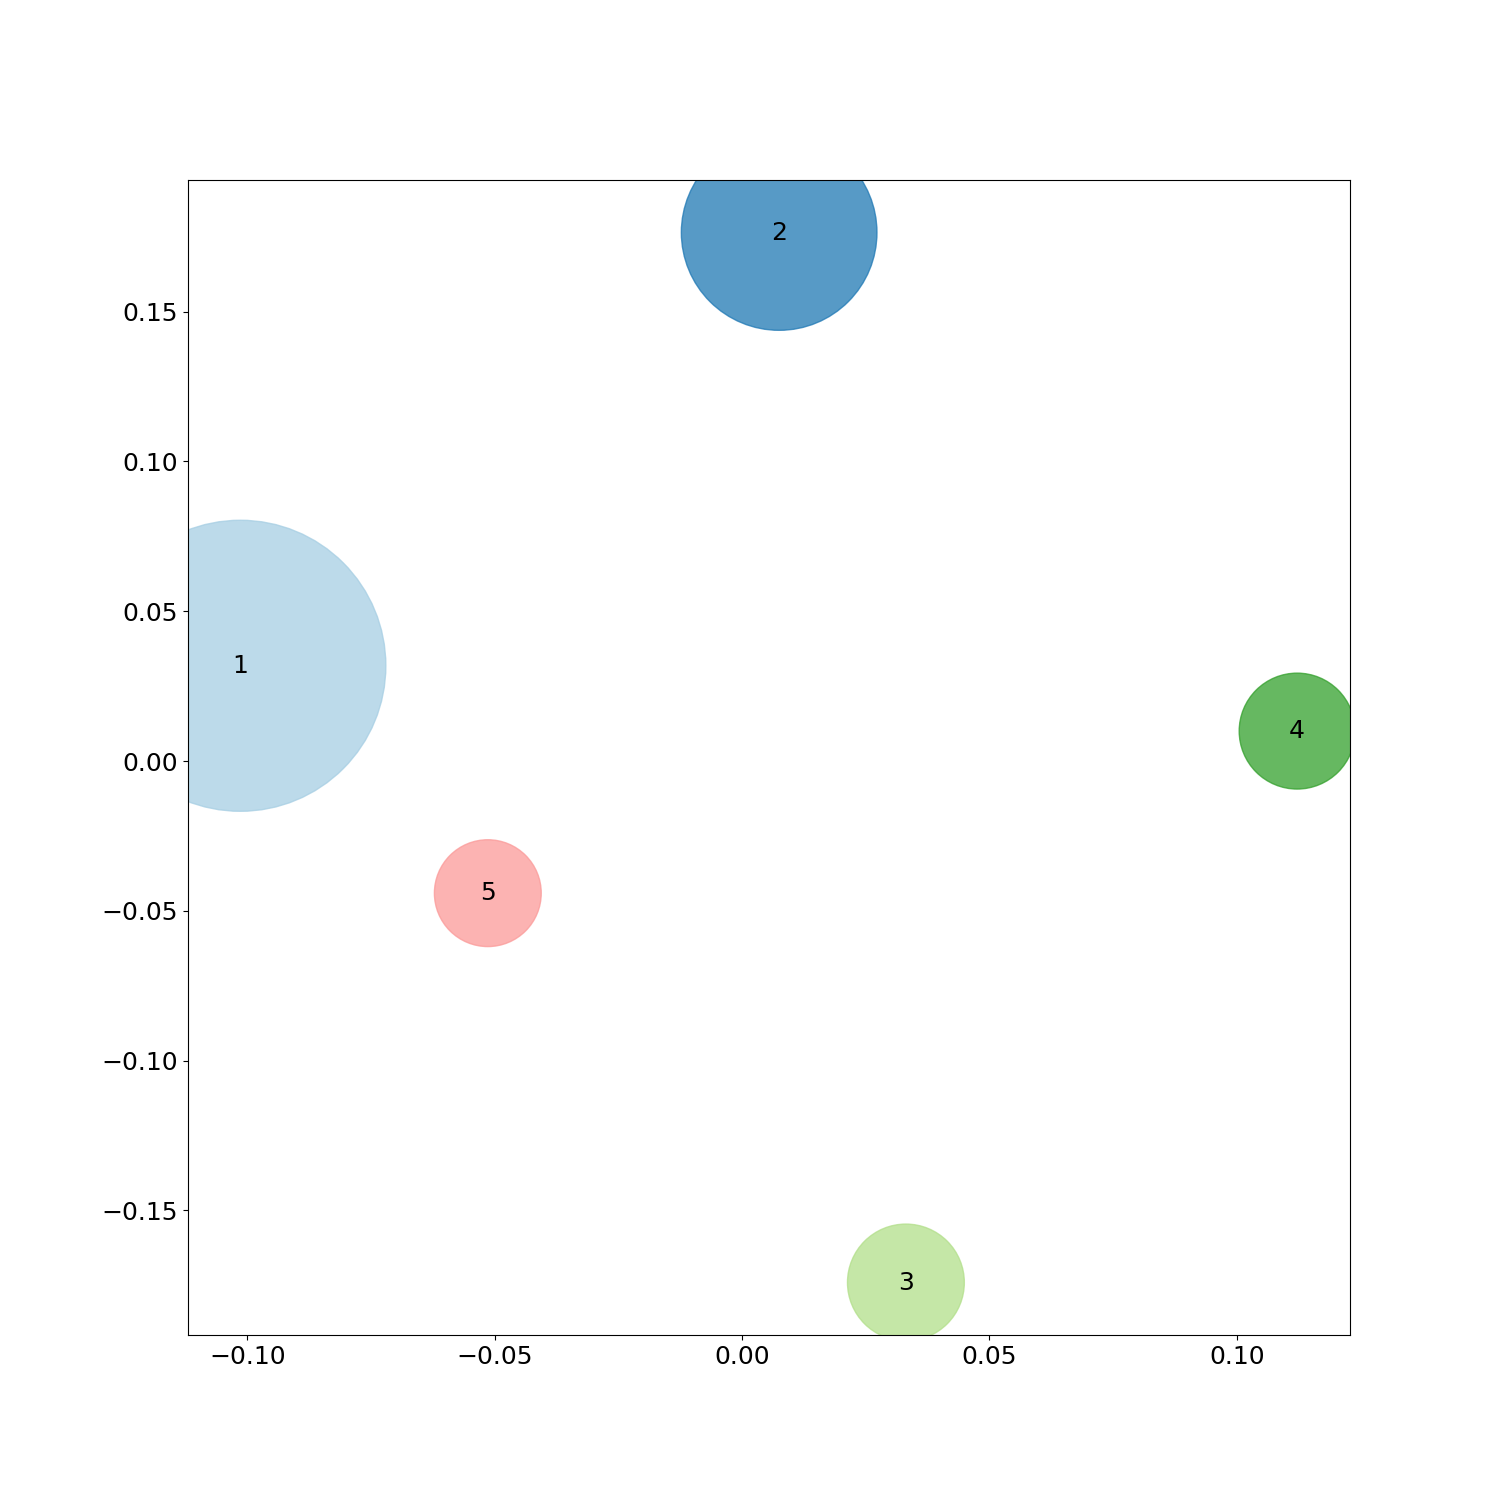
\includegraphics[scale=0.45]{caso2B/kmeans/mds.png}
\end{figure}

En \eqref{c2B_mds} se aprecia como los clusters están separados entre sí y hay un cluster más grande, otro medio y tres más pequeños.

\begin{figure}[H]
\caption{Caso 2B - Parallel coordinates de kmeans}
\label{c2B_parallel}
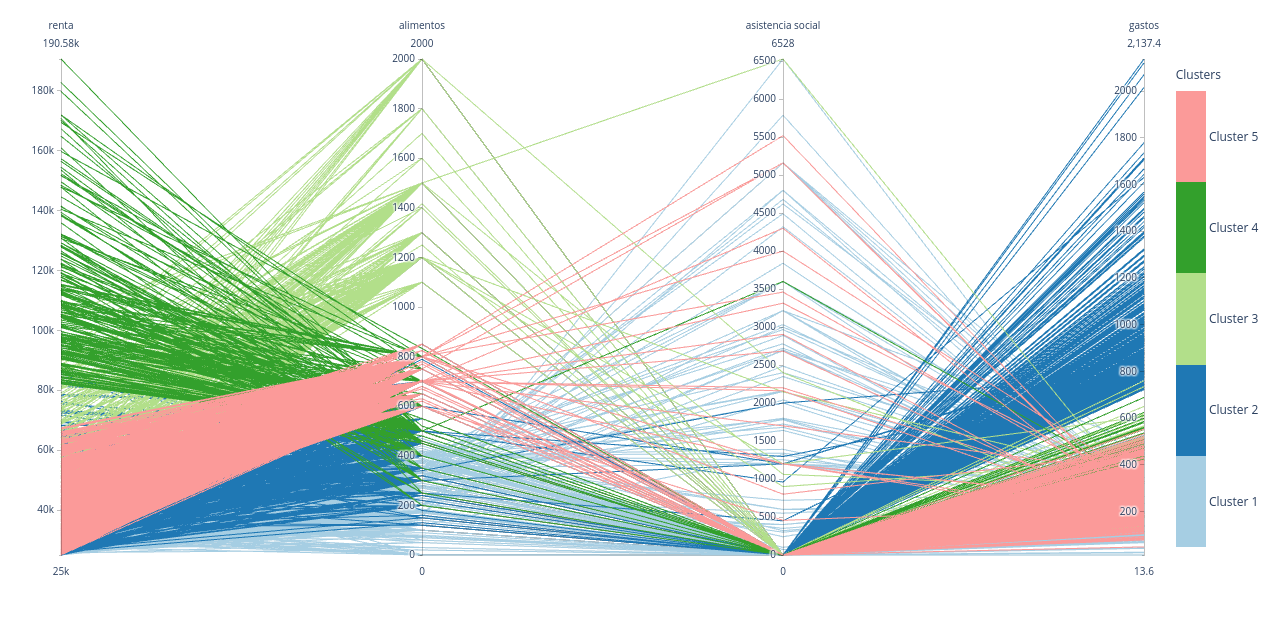
\includegraphics[scale=0.4]{caso2B/kmeans/parallel.png}
\end{figure}

En \eqref{c2B_parallel} se aprecia como el cluster verde claro  alcanza mayores valores de alimentos, como veíamos en las gráficas anteriores. De nuevo, es claro que hay dos clusters que se diferencian por sus valores altos en alimentación y gastos.

También resalta mucho en \eqref{c2B_heatmap} y \eqref{c2B_parallel} como la asistencia social, en general, es 0 salvo para algunos objetos.

En la tabla  \eqref{tab:c2B_variables} se muestran qué variables son necesarias para identificar cada cluster:

\begin{table}[H]
\centering
\caption{Caso 2B - Variables necesarias para separar el clustering en spectral cluster}
\label{tab:c2B_variables}
\begin{tabular}{ccccc}
\toprule
 Cluster & renta & alimentos & asistencia social & gastos \\
\midrule
0 & & X & & X \\
1 & & & & X \\
2 & & X & & \\
3 & X & & & \\
4 & & X & & X \\
\bottomrule
\end{tabular}
\end{table}
Como se aprecia en \eqref{tab:c2B_variables} con una sola variable en cada cluster nos sirve para diferenciarlos entre los clusters 1, 2 y 3, mientras para los clusters 0 y 4 necesitamos dos para diferenciarlos entre ellos.

\subsection{Estudio de parámetros de DBSCAN}

Vamos a analizar el comportamiento de DBSCAN según sus parámetros principales. Para ello ejecutaremos la celda de parámetros de DBSCAN, que nos proporciona las medidas obtenidas para cada par de parámetros fijados.

\begin{table}[H]
\centering
\caption{Caso 2B - Cambio de parámetros DBSCAN}
\label{tab:c2B_dbscan}
\begin{tabular}{ccccccc}
\toprule
 Algoritmo & Tiempo (s) & Silhouette & Calinski-Harabasz & Número de clusters \\
\midrule
dbscan & 0.126 & 15.000 & 2.367 & 468.250 & 0.76037 & 2 \\
dbscan & 0.126 & 20.000 & 1.638 & 473.629 & 0.75774 & 2 \\
dbscan & 0.126 & 25.000 & 1.662 & 509.168 & 0.75308 & 2 \\
dbscan & 0.126 & 30.000 & 1.580 & 520.993 & 0.75022 & 2 \\
dbscan & 0.126 & 35.000 & 1.564 & 557.247 & 0.74668 & 2 \\
dbscan & 0.130 & 15.000 & 1.676 & 444.386 & 0.76270 & 2 \\
dbscan & 0.130 & 20.000 & 1.624 & 473.629 & 0.75774 & 2 \\
dbscan & 0.130 & 25.000 & 1.622 & 473.629 & 0.75774 & 2 \\
dbscan & 0.130 & 30.000 & 1.557 & 502.252 & 0.75391 & 2 \\
dbscan & 0.130 & 35.000 & 1.516 & 543.389 & 0.74931 & 2 \\
dbscan & 0.150 & 15.000 & 1.775 & 364.846 & 0.78084 & 2 \\
dbscan & 0.150 & 20.000 & 1.693 & 401.486 & 0.77691 & 2 \\
dbscan & 0.150 & 25.000 & 1.640 & 401.486 & 0.77691 & 2 \\
dbscan & 0.150 & 30.000 & 1.701 & 419.823 & 0.77129 & 2 \\
dbscan & 0.150 & 35.000 & 1.676 & 431.335 & 0.77072 & 2 \\
dbscan & 0.170 & 15.000 & 1.725 & 326.815 & 0.78982 & 2 \\
dbscan & 0.170 & 20.000 & 1.751 & 326.815 & 0.78982 & 2 \\
dbscan & 0.170 & 25.000 & 1.852 & 343.916 & 0.78744 & 2 \\
dbscan & 0.170 & 30.000 & 1.673 & 343.916 & 0.78744 & 2 \\
dbscan & 0.170 & 35.000 & 1.713 & 343.916 & 0.78744 & 2 \\
dbscan & 0.200 & 15.000 & 1.743 & 234.734 & 0.81097 & 2 \\
dbscan & 0.200 & 20.000 & 1.728 & 236.469 & 0.80628 & 2 \\
dbscan & 0.200 & 25.000 & 1.601 & 274.152 & 0.80115 & 2 \\
dbscan & 0.200 & 30.000 & 1.732 & 277.749 & 0.79948 & 2 \\
dbscan & 0.200 & 35.000 & 1.686 & 309.161 & 0.79346 & 2 \\
\bottomrule
\end{tabular}
\end{table}

Como podemos apreciar en \eqref{tab:c2B_dbscan} DBSCAN siempre realiza dos clusters. El tamaño de estos es siempre similar, más del $90\%$ los ejemplos están agrupados en el cluster $0$ y los restantes están en el $-1$.

Este algoritmo no ha hecho ninguna buena agrupación en ningún caso de los probados, pese a que, de nuevo su silhouette es bastante alto.

No podemos interpretar demasiado Calinsk-Harabasz, ya que al no estar normalizado no sabemos si los valores dados son muy altos. Sí podemos decir que los mejores agrupamientos (que han proporcionado un valor de esta medida más alto) se han dado cuando min samples es $35$.


\subsection{Estudio de parámetros de Kmeans}

Estudiamos ahora el algoritmo Kmeans. Se ha variado el número de clusters.

\begin{table}[H]
\centering
\caption{Caso 2B - Cambio de parámetros Kmeans}
\label{tab:c2B_kmeans}
\begin{tabular}{cccccc}
\toprule
Algoritmo & n clusters & Tiempo(s) & Silhouette & Calinski-Harabasz & n clusters \\
\midrule
kmeans & 3.000 & 0.392 & 3085.841 & 0.39834 & 3 \\
kmeans & 4.000 & 0.243 & 3065.400 & 0.40218 & 4 \\
kmeans & 5.000 & 0.407 & 2962.319 & 0.30911 & 5 \\
kmeans & 6.000 & 0.441 & 2878.260 & 0.31752 & 6 \\
kmeans & 7.000 & 0.496 & 2799.096 & 0.31771 & 7 \\
kmeans & 8.000 & 0.508 & 2760.228 & 0.27617 & 8 \\
kmeans & 9.000 & 0.787 & 2707.579 & 0.27781 & 9 \\
kmeans & 10.000 & 0.891 & 2620.283 & 0.27880 & 10 \\
\bottomrule
\end{tabular}
\end{table}

Podemos ver en \eqref{tab:c2B_kmeans} como las medidas comienzan subiendo hasta que el número de clusters es 4, donde alcanzan su máximo Silhouette y Calinski-harabasz, para después volver comenzar a decrementarse.

Asimismo el tiempo de ejecución se incrementa a la par que el número de clusters crece, pues hay que hacer más cálculos.

A la vista de estas medidas, parece que la mejor agrupación sería con 4 clusters.


\section{Interpretación de la segmentación}

Una variable bastante relevante al comparar estos casos ha sido la asistencia social, ya que en el caso de rentas altas la mayor parte de objetos no recibían (valía 0), mientras para rentas bajas ha sido muy relevante a la hora de realizar agrupamientos.

En ambos casos los gastos y alimentación han servido para separar dos clusters del resto usando solamente una de ellas. Si comparamos ambas, usando por ejemplos \eqref{c2A_scatter} y \eqref{c2B_scatter} vemos que en el caso de alimentación para rentas altas se considera un valor "alto" de esta variable a partir de $1000$, mientras para rentas bajas es $400$. Igualmente, para gastos en rentas altas el valor de corte es en torno a $500$, pero para rentas bajas se considera más o menos $350$.

Además, vemos como en general los valores de gastos y alimentación son considerablemente más altos para rentas altas que para rentas bajas.

Para separar los otros clusters usamos dos variables, donde una de ellas es la renta, por lo tanto es de menos utilidad al compararlos, ya que la renta está sesgada en cada caso de estudio.

Así, vemos como las personas con rentas más altas prácticamente no tienen ayudas sociales y gastan más en alimentos y gastos de alquiler y similares, mientras las personas con rentas bajas cuentan con más ayudas sociales y gastan menos en alimentación y gastos del hogar.





%\ctparttext{\color{black}\begin{center}
%		Esta es una descripción de la parte de informática.
%\end{center}}

%\part{Parte de informática}
\chapter{Caso 3: Personas con hipoteca, alquiler o cesión gratuita}

\section{Descripción del caso de estudio}
En este caso de estudio se han elegido las respuestas para las que el régimen de tenencia es distinto de en propiedad sin hipoteca, es decir, pueden estar en propiedad con hipoteca, en alquiler a precio de mercado o inferior o en cesión gratuita.

Se pretende estudiar las relaciones entre gastos en la hipoteca o alquiler, alimentación, número de miembros y ayudas sociales.

Las variables que se van a seleccionar para realizar el análisis son:
\begin{itemize}
\item \textbf{Renta}: Renta disponible total del hogar en el año anterior al de encuesta.
\item \textbf{Alimentos}: Durante el mes pasado, ¿cuál fue aproximadamente el importe que el hogar gastó en alimentos y bebidas no alcohólicas para ser consumidas en casa?
\item \textbf{Asistencia social}: Ingresos por asistencia social en el año anterior al
de encuesta.
\item \textbf{Gastos}: Gastos de la vivienda: Alquiler (si la vivienda se encuentra en régimen de alquiler), intereses de la hipoteca (para viviendas en propiedad con pagos pendientes) y otros gastos asociados (comunidad, agua, electricidad, gas, etc.)
\item \textbf{Número de miembros}: Número de miembros del hogar.
\end{itemize}

Este caso de estudio consta de $7295$ respuestas a la encuesta, cada una con las $5$ variables indicadas.

\section{Ejecución de algoritmos}

Las diferentes medidas obtenidas para cada algoritmo se muestran en \eqref{tab:c3_alg}.

\begin{table}[H]
\centering
\caption{Caso 3 - Resultados de ejecución de algoritmos.}
\label{tab:c3_alg}
\begin{tabular}{ccccc}
\toprule
 Algoritmo & Tiempo (s) & Calinski-Harabasz & Silhouette & Número de clusters \\
\midrule
kmeans & 0.145 & 3108.765 & 0.28264 & 5 \\
birch & 0.277 & 668.429 & 0.35988 & 5 \\
spectral & 10.964 & 2192.446 & 0.28476 & 5 \\
dbscan & 0.801 & 310.408 & 0.57966 & 2 \\
meanshift & 58.323 & 140.587 & 0.28696 & 15 \\
\bottomrule
\end{tabular}
\end{table}

Al igual que en los otros casos, meanshift sigue tardando mucho más tiempo que el resto de algoritmos, seguido por spectral cluster. Llama la atención que DBSCAN en este caso ha resultado mucho más lento que en los anteriores, aunque sigue sin llegar a un segundo. Kmeans y birch han tardado tiempos similares.

De nuevo, DBSCAN ha hecho una agrupación mala en dos clusters, el cluster $0$ con el $89.51\%$ de los objetos y los restantes en el cluster $-1$.

Meanshift ha agrupado los objetos en 15 clusters, y ha obtenido un valor de calinski-harabasz bastante bajo en comparación con los demás algoritmos, lo que hace sospechar que su agrupación no va a ser demasiado buena. Mirando el tamaño de los clusters generados ha realizado uno con el $94.67\%$ de los elementos, y el resto los ha agrupado en clusters con tamaños inferiores al $2.6\%$. Por tanto, a pesar de que su silhouette no sea especialmente bajo en comparación con los otros algoritmos, parece que el clustering ha sido bastante malo.

De entre los tres algoritmos restantes, pese a que birch tiene el mayor silhouette, su calinski-harabasz es muy bajo. Y entre kmeans y spectral clustering, dado que tienen valores de silhouette similares, a priori kmeans habría realizado mejor agrupamiento, pues su calinski-harabasz es mayor.


\section{Análisis}


Para el análisis nos basaremos en los resultados de kmeans, pues ha obtenido, en principio, los mejores resultados en la ejecución. Este algoritmo genera 5 clusters. cuatro con tamaño similar y uno más pequeño, como se puede ver en \eqref{c3_tam}

\begin{figure}[H]
\caption{Caso 3- Tamaño de los clusters generados por kmeans}
\label{c3_tam}
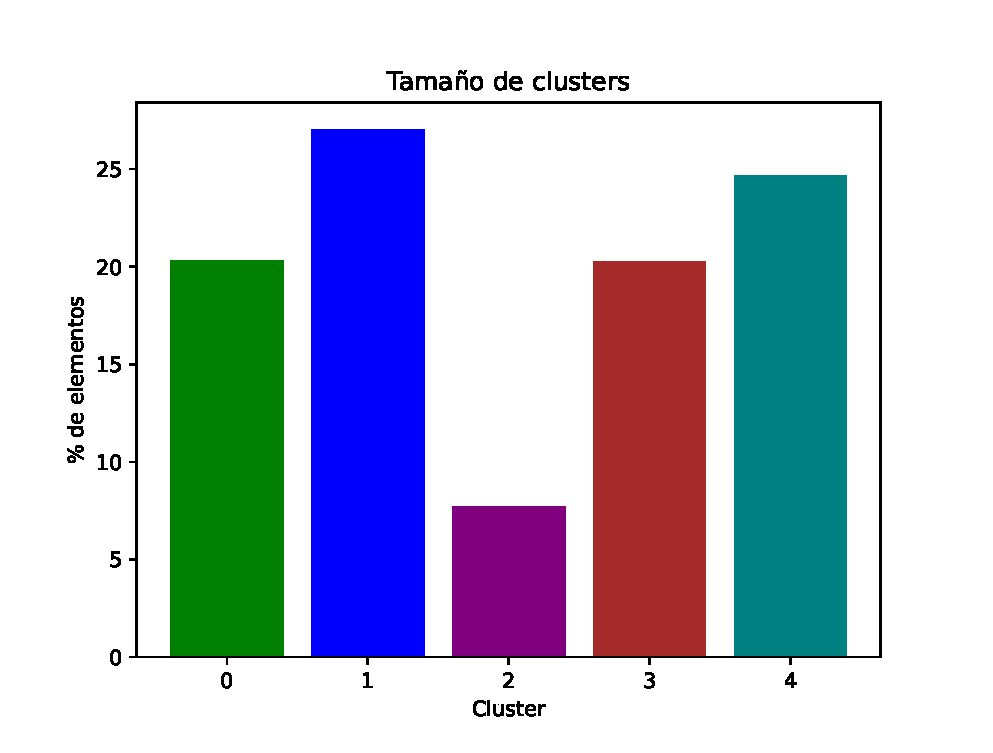
\includegraphics[scale=1]{caso3/kmeans/bar.eps}
\end{figure}

Ahora estudiamos la scatter matrix \eqref{c3_scatter}:

\begin{figure}[H]
\caption{Caso 3- Scatter matrix de kmeans}
\label{c3_scatter}
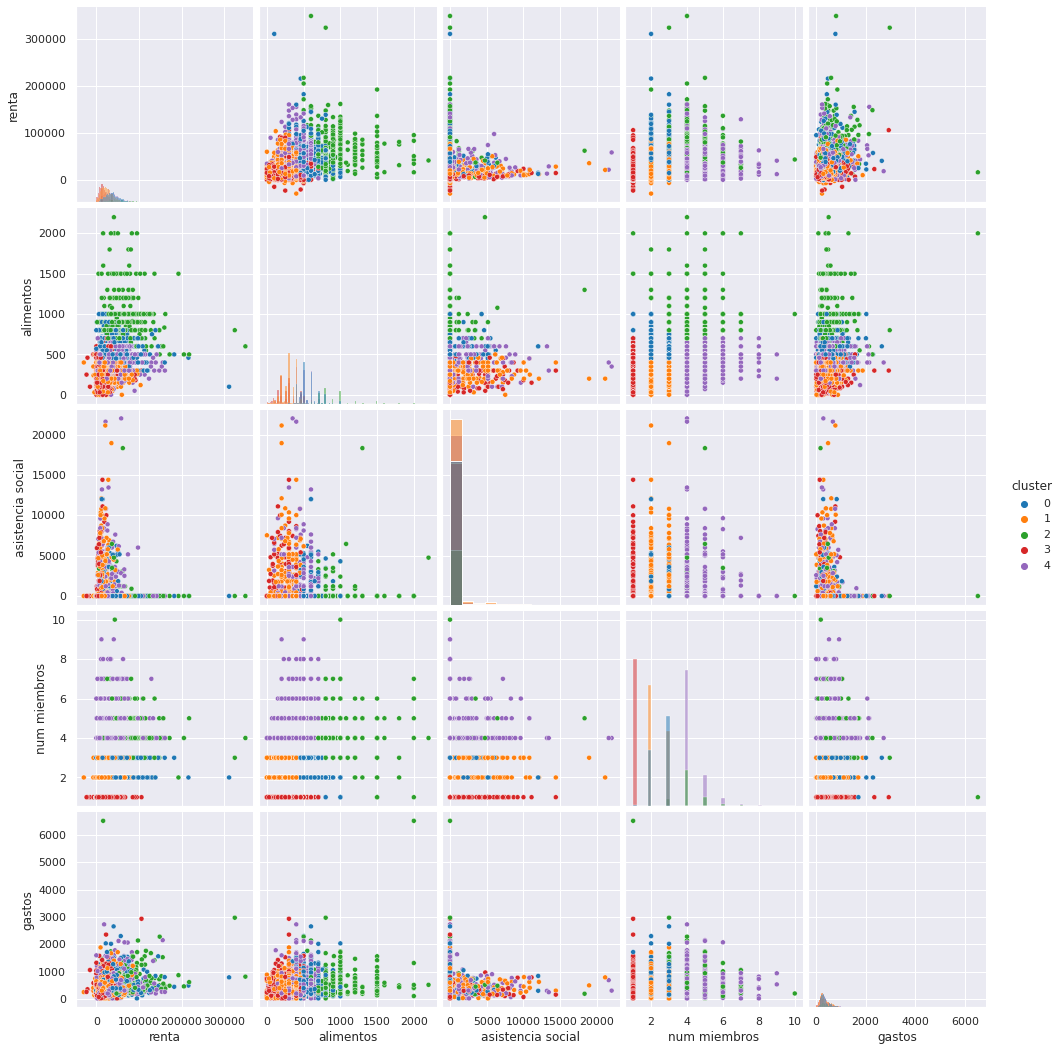
\includegraphics[scale=0.45]{caso3/kmeans/scatter.png}
\end{figure}

Analizamos \eqref{c3_scatter}, obteniendo así una distinción relativamente clara de los clusters. El cluster 2, de color verde, solo requiere una variable para identificarse, la de alimentos, mientra que los demás pueden distinguirse entre ellos usando solamente alimentos y el número de miembros del hogar.

Llama la atención sobre esta gráfica como el número de miembros, al ser una variable discreta, los puntos se encuentran alineados en los valores enteros.

\begin{figure}[H]
\caption{Caso 3- Heatmap de kmeans}
\label{c3_heatmap}
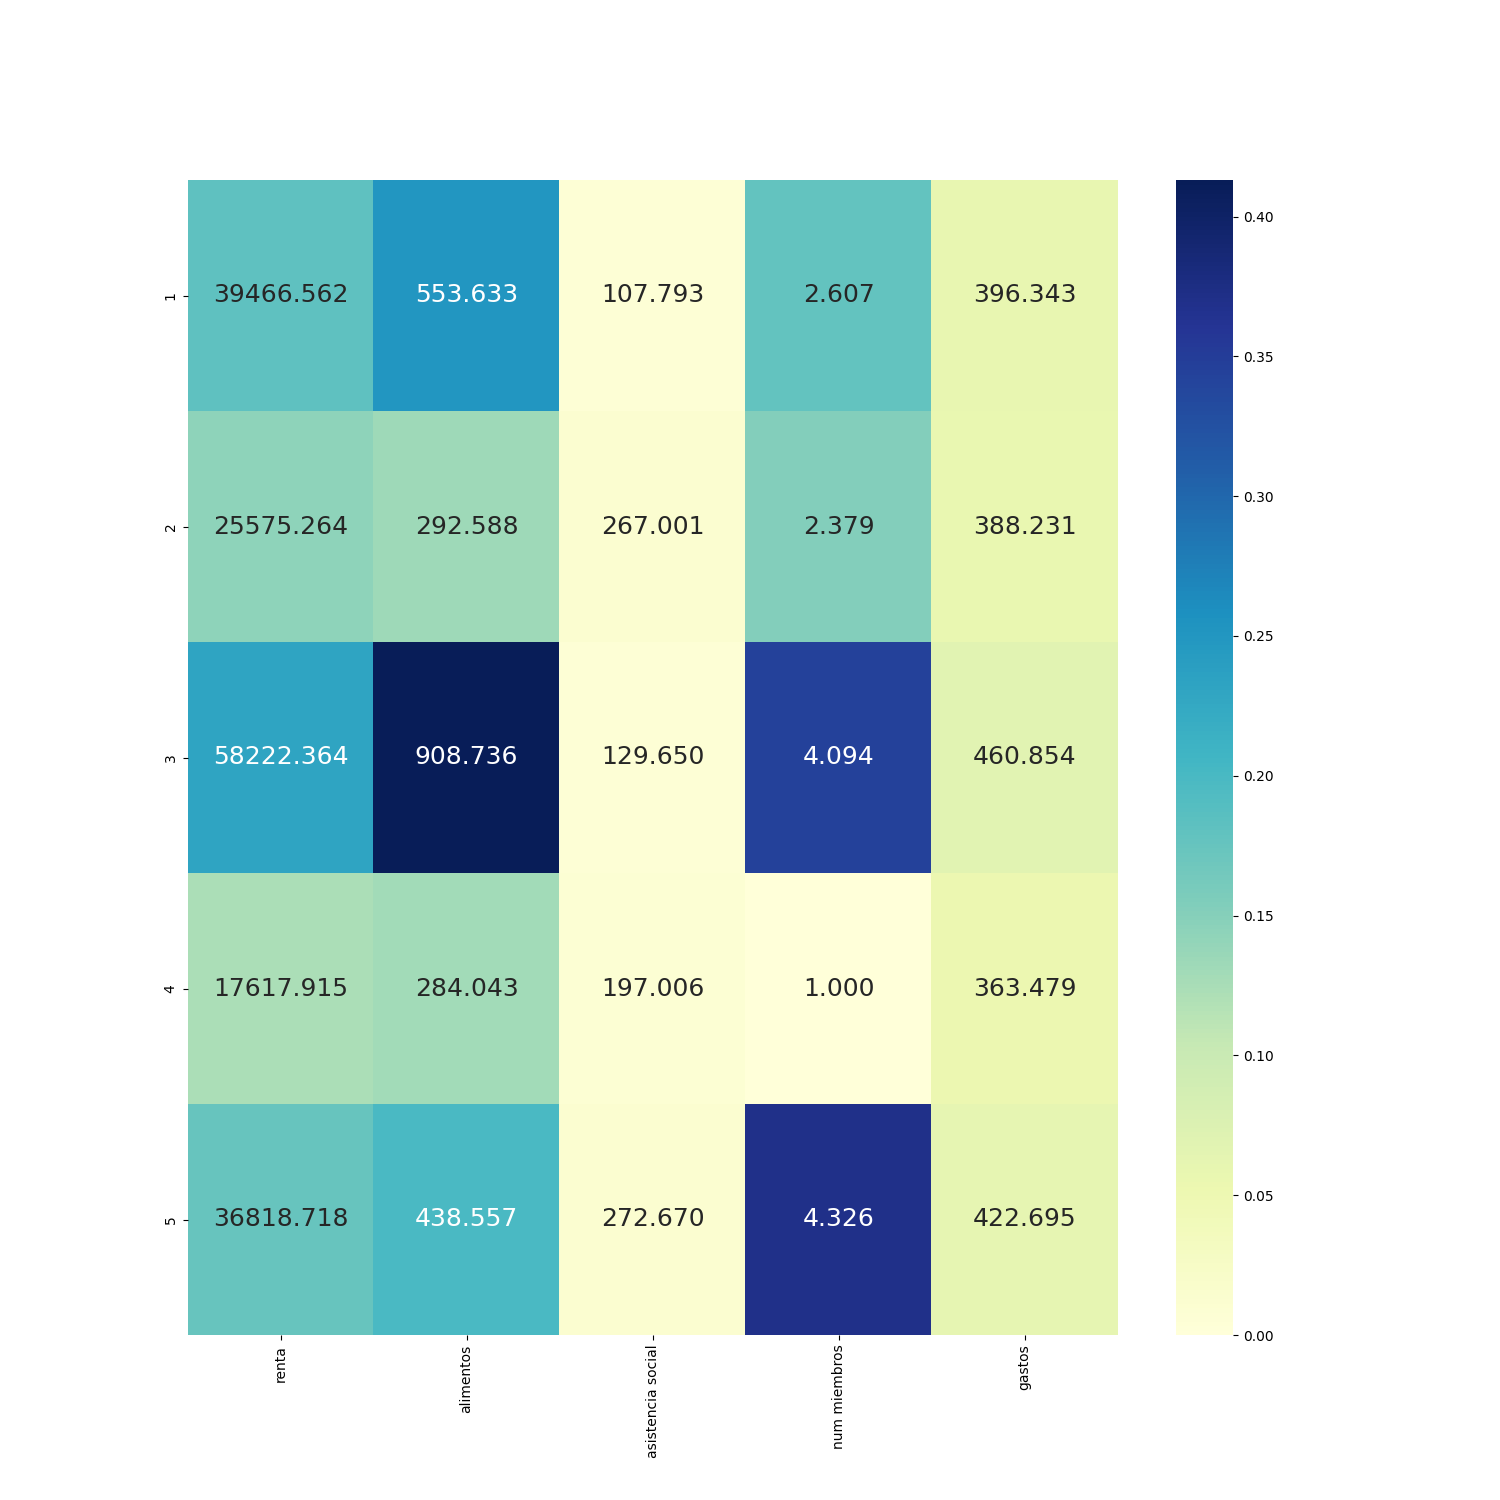
\includegraphics[scale=0.45]{caso3/kmeans/heatmap.png}
\end{figure}

En \eqref{c3_heatmap} podemos observar como el cluster 3 toma valores en general mayores en alimentos que los otros clusters.

Sin embargo, pese a que en la scatter matrix \eqref{c3_scatter} se distinguieran bien los clusters solamente usando alimentos y número de miembros, en el heatmap esta división no se ve tan clara, aunque si se aprecia que el cluster 4 (que en la scatter matrix es el 3) el número de miembros del hogar es 1. Y el cluster 5 puede distnguirse del 1, 2 y 4 usando el número de miembros, y del 3 mediante el número de alimentos.


\begin{figure}[H]
\caption{Caso 3- MDS de kmeans}
\label{c3_mds}
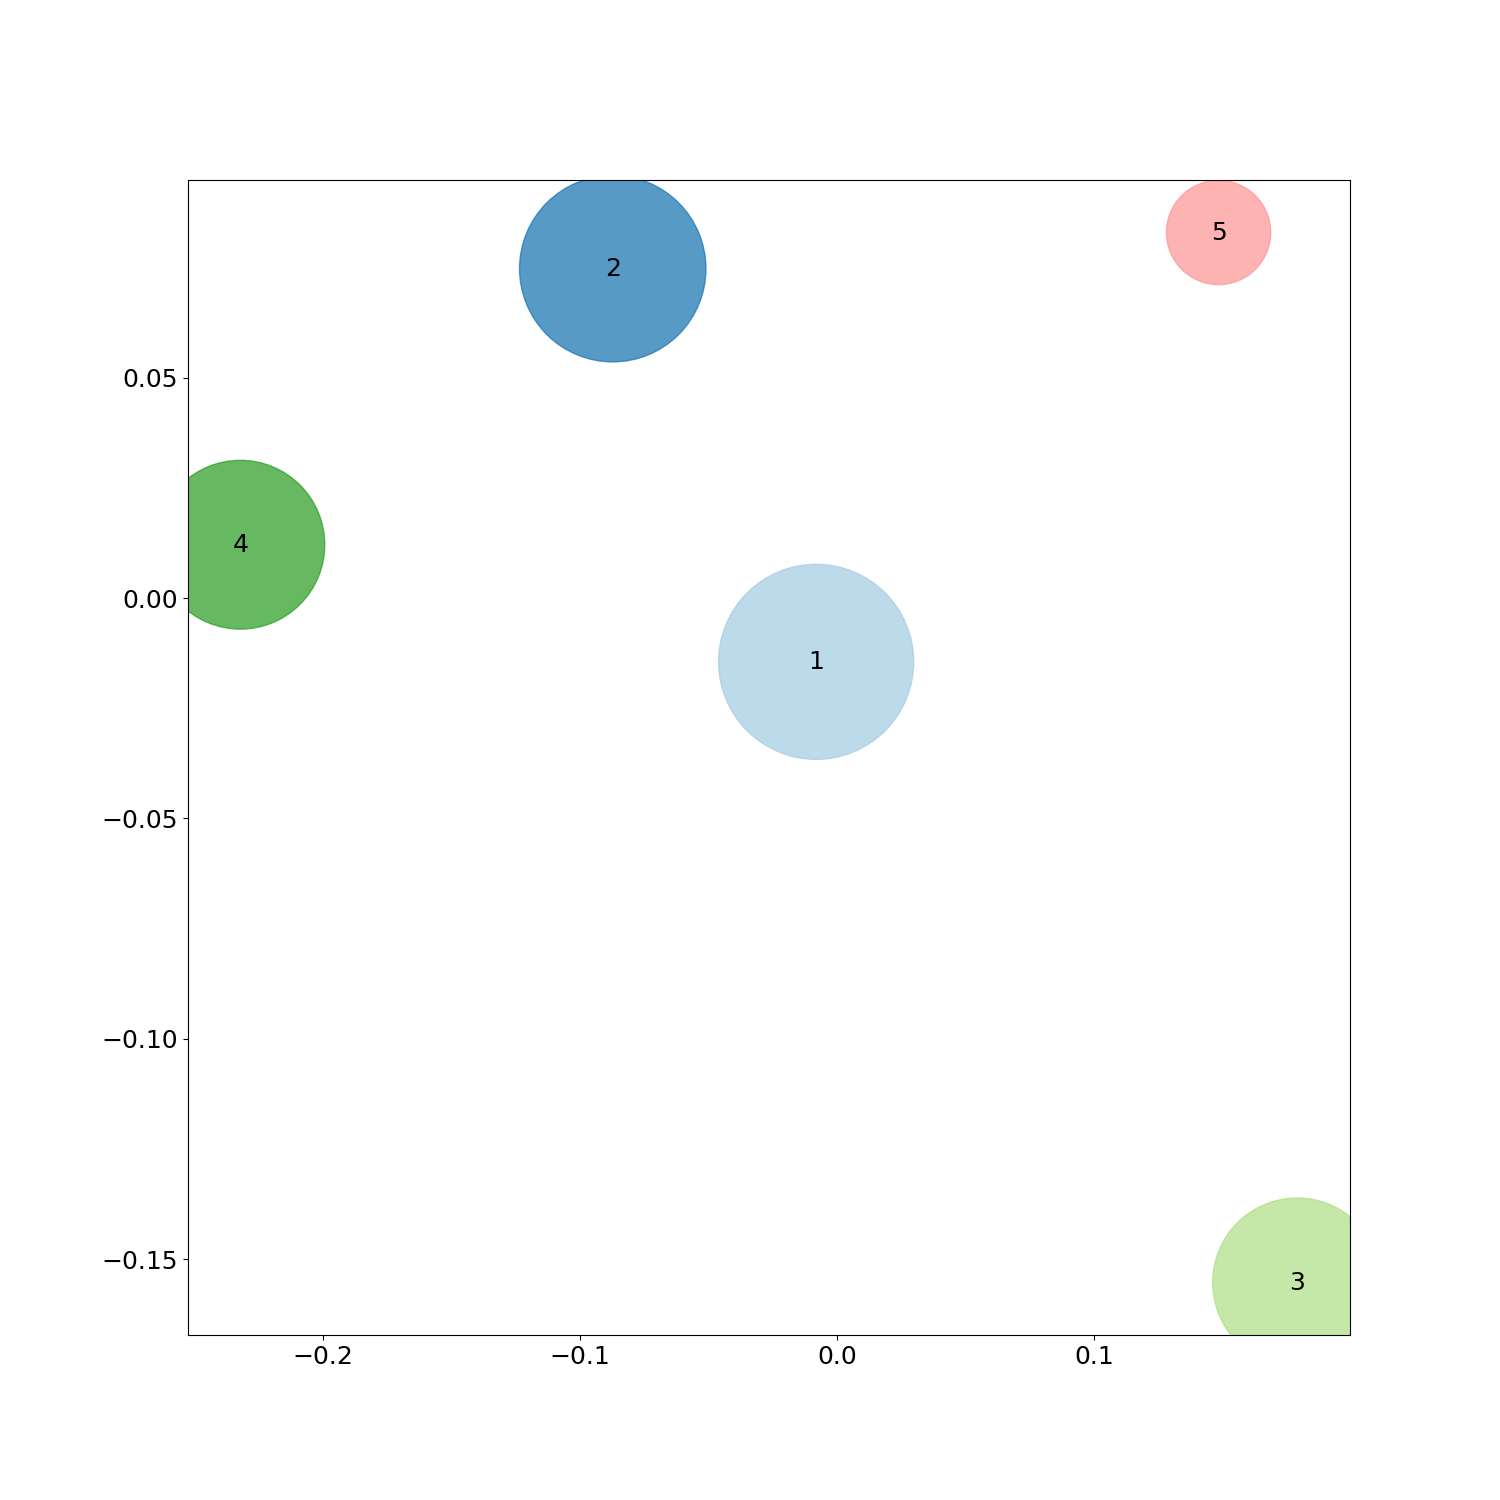
\includegraphics[scale=0.45]{caso3/kmeans/mds.png}
\end{figure}

En \eqref{c3_mds} se aprecia como los clusters están notablemente separados y con tamaños bastante similares.

\begin{figure}[H]
\caption{Caso 3- Parallel coordinates de kmean}
\label{c3_parallel}
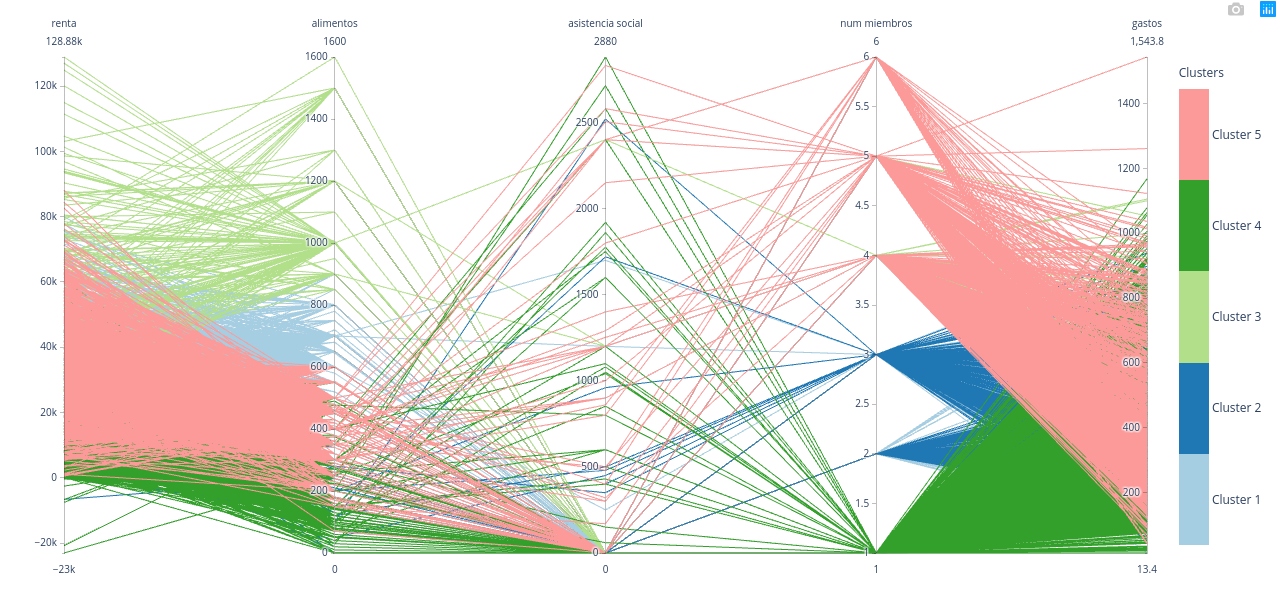
\includegraphics[scale=0.4]{caso3/kmeans/parallel.png}
\end{figure}

Finalmente, en \eqref{c3_parallel} se aprecia muy bien como el número de miembros toma valores discretos, pues se agrupan las líneas en los números enteros de esta columna. También se ve claramente como el cluster verde claro, que es el 3, toma valores mucho más altos en alimentos que el resto, aunque es algo disperso. El cluster rosa, correspondiente al 5 es menos disperso y toma valores de número de miembros más altos que los otros clusters.

Si combinamos de nuevo la información de las líneas que llegan a alimentos y número de miembros, obtenemos los mismos resultados que mediante la scatter matrix.



En la tabla  \eqref{tab:c3_variables} se muestran qué variables son necesarias para identificar cada cluster:

\begin{table}[H]
\centering
\caption{Caso 3 - Variables necesarias para separar el clustering en kmeans}
\label{tab:c3_variables}
\begin{tabular}{cccccc}
\toprule
 Cluster & renta & alimentos & asistencia social & num miembros & gastos \\
\midrule
0 & & X & & X & \\
1 & & X & & X & \\
2 & & X & & & \\
3 & & X & & X & \\
4 & & X & & X & \\
\bottomrule
\end{tabular}
\end{table}
Como se aprecia en \eqref{tab:c3_variables} con solo la variable alimentos distinguimos el cluster 2, y con alimentos y num miembros separamos los demás.

\section{Estudio de parámetros de spectral cluster}

Vamos a estudiar el comportamiento de spectral cluster variando el número de clusters que va a realizar.

\begin{table}[H]
\centering
\caption{Caso 3 - Cambio de parámetros Spectral cluster}
\label{tab:c3_spectral}
\begin{tabular}{ccccccc}
\toprule
Algoritmo & num clusters & Tiempo(s) & Calinski-Harabasz & Silhouette & n clusters \\
\midrule
spectral & 3 & 10.986 & 3763.346 & 0.33783 & 3 \\
spectral & 4 & 10.916 & 2634.019 & 0.30196 & 4 \\
spectral & 5 & 10.949 & 2192.446 & 0.28476 & 5 \\
spectral & 6 & 10.964 & 1599.167 & 0.20130 & 6 \\
spectral & 7 & 11.258 & 1669.853 & 0.19525 & 7 \\
spectral & 8 & 11.180 & 1766.949 & 0.20175 & 8 \\
spectral & 9 & 11.662 & 1525.245 & 0.17595 & 9 \\
spectral & 10 & 11.725 & 1425.793 & 0.17855 & 10 \\
\bottomrule
\end{tabular}
\end{table}

Observamos que el mayor valor de silhouette se da cuando se realizan 3 clusters, así como el mayor valor de Calinski-harabasz. Por tanto, en principio este es el mejor agrupamiento que ha realizado spectral cluster. Si miramos lso tamaños de los clusters generados vemos que son $40.11\%$, $40.08\%$ y $19.81\%$, es decir, están equilibrados dos de ellos y el tercero es algo más pequeño. No parece a priori un mal clustering.

El resto de ejecuciones de spectral cluster también genera clusters de tamaños relativamente equilibrados.

Finalmente, cabe destacar que el tiempo de ejecución se incrementa a medida que el número de clusters aumenta, pero no en una medida exagerada.


\section{Estudio de parámetros de Meanshift}

Estudiamos ahora el algoritmo Meanshift. Se ha ido variando el radio (bandwith) del algoritmo, siendo la primera entrada en la tabla el que se calcula automáticamente al ejecutar el algoritmo.

\begin{table}[H]
\centering
\caption{Caso 3 - Cambio de parámetros Meanshift}
\label{tab:c3_meanshift}
\begin{tabular}{cccccc}
\toprule
Algoritmo & bandwith & Tiempo(s) & Calinski-Harabasz & Silhouette & n clusters \\
\midrule
meanshift & 0.175 & 58.453 & 140.587 & 0.28696 & 15 \\
meanshift & 0.050 & 55.001 & 251.495 & 0.15194 & 445 \\
meanshift & 0.100 & 48.993 & 294.485 & 0.25028 & 120 \\
meanshift & 0.200 & 40.302 & 106.456 & 0.35944 & 13 \\
meanshift & 0.300 & 38.224 & 62.198 & 0.57110 & 7 \\
meanshift & 0.400 & 27.835 & 95.624 & 0.69156 & 3 \\
meanshift & 0.500 & 23.839 & 36.994 & 0.79705 & 2 \\
meanshift & 0.600 & 20.824 & 36.994 & 0.79705 & 2 \\
meanshift & 0.700 & 18.235 & 36.994 & 0.79705 & 2 \\
meanshift & 0.800 & 15.558 & 36.994 & 0.79705 & 2 \\
meanshift & 0.900 & 15.321 &  &  & 1 \\
meanshift & 1 & 15.092 &  &  & 1 \\
\bottomrule
\end{tabular}
\end{table}


En la primera entrada de la tabla se encuentra el radio calculado automáticamente, que genera 15 clusters. Como se comentó al analizar los algoritmos en general para este caso de estudio, no realiza un buen agrupamiento por los tamaños de los clusters.

Es llamativo como a medida que aumenta el radio, el número de clusters se reduce. Los casos más razonables parecen cuando el radio vale $0.3$ y se generan 7 clusters y cuando vale $0.4$ y se generan 3, pero mirando los tamaños de los clusters generados observamos que en ambos casos se genera un cluster con más del $99.5\%$ de los objetos y el resto se agrupa en los clusters restantes. Esto indica que no es un buen agrupamiento.

Finalmente, vemos como el tiempo se reduce drásticamente conforme lo hace el número de clusters generados.



\section{Interpretación de la segmentación}


Fijándonos en los resultados obtenidos, podemos concluir que las variables más relevantes en este caso han sido el número de miembros del hogar y el gasto en alimentación, pues solamente con ellas se pueden distinguir todos los clusters.

Además, los clusters están bastante separados, lo que puede deberse en gran parte a que el número de miembros solo toma valores enteros naturales, lo que puede estar forzando una separación usando esta variable e incrementando el silhouette artificialmente, pues premia mucho la separación entre los clusters.

Finalmente cabe destacar que al contrario de lo que podríamos haber pensado en un principio, la renta o los gastos en la casa y el número de miembros por familia no producen tan buena agrupación como lo hace la alimentación.







%\chapter{Modelos básicos en epidemiología}

\section{Tipos de modelos}

Los modelos discretos (principalmente SI, SIR y SIS) usan los estados Susceptible, Infectado y Recuperado. Los nombres suelen hacer referencia al flujo que se sigue para pasar entre los estados. Así, por ejemplo un modelo SI pasa de susceptible a infectado, uno SIR de susceptible a infectado y recuperado y SIS alterna entre susceptible e infectado.

En estos modelos se hacen dos suposiciones:
\begin{enumerate}
\item La población se mezcla de manera homogénea, es decir, todos los individuos tienen la misma probabilidad de contraer la enfermedad.
\item El total de la población es constante y lo denotaremos por $N$.
\end{enumerate}

En este capítulo estudiaremos los principales modelos epidemiológicos discretos y sus equivalentes continuos.

\section{Modelo SI}
El modelo SI es el modelo más simple de todos. Los individuos nacen siendo susceptibles a una enfermedad, y una vez infectados permanecen infectados el resto de su vida.
Un ejemplo de una enfermedad que pueda modelarse usando SI es el herpes.

Las siguientes ecuaciones describen el modelo SI discreto:

\begin{equation}
\label{eqn: SI}
\begin{aligned}
S_{n+1}=S_n\left( 1-\frac{\alpha\Delta t}{N}I_n\right) \\
I_{n+1}=I_n\left( 1+\frac{\alpha\Delta t}{N}S_n\right)
\end{aligned}
\end{equation}

donde $S_n$ indica el número de individuos susceptibles en el instante $t_n$, e $I_n$ hace referencia al número de individuos infectados en ese instante. $\Delta t$ es el tiempo transcurrido entre dos instantes $t_{n+1}-t_n$, y N es el tamaño total de la población, con condiciones iniciales $S_0>0$, $I_0>0$ y $S_0+I_0=N$.

En estas ecuaciones $\alpha$ es la tasa de contacto; es decir, el número medio de individuos con los que un infectado tiene suficiente contacto para contagiarlo en un intervalo de tiempo. Por tanto, $S_n$ representa el número de individuos susceptibles en el tiempo $n\Delta t$.

Pasaremos a imponer las suposiciones descritas anteriormente para estos modelos. En primer lugar, suponemos que la población se mezcla de manera homogénea de ahora en adelante. Para imponer la segunda suposición, la población total se mantiene constante, siendo trivial que se cumpla siempre, ya que sumando el sistema de ecuaciones el resultado es $N$ y asumimos que las soluciones son siempre positivas dado que las soluciones negativas no tienen sentido, ya que sería hablar de un número negativo de individuos, ya sean infectados, recuperados o susceptibles de contraer la enfermedad.

\begin{lemma}
$S_n$ es monótonamente decreciente e $I_n$ es monótonamente creciente.
\end{lemma}

\begin{proof}
$S_{n+1}$ es $S_n$ multiplicado por un valor menor que $1$, mientras que $I_{n+1}$ corresponde a $I_n$ multiplicado por un valor mayor que $1$.
\end{proof}

\begin{proposition}
Las soluciones de las ecuaciones \eqref{eqn: SI} son positivas si y solo si $\alpha\Delta t \leq 1$.
\end{proposition}

\begin{proof}
Supongamos que $I_n, S_n > 0$. Por la segunda ecuación del modelo \eqref{eqn: SI} es claro que $I_{n+1}>0$, pues $S_n>0$ y $1+\frac{\alpha\Delta t}{N}>0$.

Para la primera ecuación tenemos que $S_{n+1} > 0$ si y solo si
$$1-\frac{\alpha\Delta t}{N}I_n >0,$$

ya que $S_n$ es positivo por hipótesis. Esto equivale a $N>\alpha \Delta t I_n$, y puesto que $S_n+I_n=N$ se tiene:
$$N>\alpha\Delta t(N-S_n),$$
esto es
$$\alpha\Delta t S_n > (\alpha\Delta t -1) N.$$
Como $\alpha\Delta t S_n > 0$, tenemos entonces que la desigualdad se da para todo $n$ si y solo si:
$$\alpha\Delta t -1 \leq 0 \Leftrightarrow \alpha\Delta t \leq 1.$$
\end{proof}


Buscamos ahora ver cual es el comportamiento del sistema, calculando los puntos de equilibrio; esto es, las soluciones constantes en el tiempo, resolviendo:

$$
\begin{aligned}
S^*=S^*\left( 1-\frac{\alpha\Delta t}{N}I^*\right) \\
I^*=I^*\left( 1+\frac{\alpha\Delta t}{N}S^*\right) \\
S^*+I^*=N
\end{aligned}
$$

Los únicos puntos de equilibrio posibles son: $(S^*,I^*)=(0,N)$ y $(S^*,I^*)=(N,0)$. Puesto que las condiciones iniciales son positivas y como $S_n$ es monótonamente decreciente e $I_n$ es monótonamente creciente, así $S_{n+1}<S_n$ y $I_{n+1}>I_n$ para cualquier $n\in\mathbb{N}$, entonces debe converger a $(S^*,I^*)=(0,N)$, pues son sucesiones monótonas acotadas.

Expresando $\alpha$ como una tasa podemos obtener las ecuaciones diferenciales análogas de la siguiente manera. Considerando

$$\frac{S_{n+1} - S_n}{\Delta t} \approx S'(t),$$

El análogo continuo al sistema \eqref{eqn: SI} viene dado por:

\begin{equation}
\begin{aligned}
S'(t) = -\frac{\alpha}{N}SI \\
I'(t) = \frac{\alpha}{N}SI
\end{aligned}
\end{equation}

con condiciones iniciales $S(0)+I(0)=N$.

Calculamos los puntos de equilibrio de manera análoga al caso discreto, es decir, suponemos que las funciones son constantes y, resolviendo el sistema de ecuaciones, podemos comprobar que las soluciones convergen a $(S^*,I^*)=(0,N)$ y, por tanto, tienen el mismo comportamiento que el caso discreto.

Sustituyendo en el modelo $S=N-I$ obtenemos la ecuación diferencial logística

$$I'(t) = I\frac{\alpha}{N}(N-I).$$

Esta ecuación diferencial se puede resolver por separación de variables como sigue:

\begin{equation}
\begin{aligned}
I'(t)=\frac{\alpha}{N}I(N-I(t)) & \Leftrightarrow \int \frac{dI}{I(N-I)} = \int \frac{\alpha}{N} dt \\
& \Leftrightarrow \frac{1}{N}\int \left(\frac{1}{I}+\frac{1}{N-I}\right) dI = \frac{\alpha}{N}t+c \\
& \Leftrightarrow  \frac{1}{N}\log{\frac{I}{N-I}} = e^{\frac{\alpha}{N}t+c} \\
& \Leftrightarrow  \frac{I}{N-I} = e^ce^{\alpha t} \\
& \Leftrightarrow  I = e^ce^{\alpha t}(N-I) \\
& \Leftrightarrow  I(1+e^ce^{\alpha t}) = e^ce^{\alpha t}N \\
& \Leftrightarrow  I(t) = \frac{e^ce^{\alpha t}N}{1+e^ce^{\alpha t} }
\end{aligned}
\end{equation}

Usando el valor inicial $I(0)$ tenemos:

\begin{equation}
\begin{aligned}
I(0) = \frac{e^cN}{1+e^c} & \Leftrightarrow (1+e^c)I(0) = e^cN \\
& \Leftrightarrow e^c(N-I(0)) = I(0) \\
& \Leftrightarrow e^c = \frac{I(0)}{N-I(0)}
\end {aligned}
\end{equation}

luego la solución general es:

$$I(t) = \frac{I(0)e^{\alpha t}N}{(N-I(0))+I(0)e^{\alpha t}} = \frac{I(0)N}{(N-I(0))e^{-\alpha t}+I(0)}$$

Es claro que $I$ tiende monótonamente a $N$, luego tiene el mismo comportamiento que el modelo discreto.


\begin{figure}
\begin{center}
\caption{Gráfica del modelo SI discreto, en una población total de $100$ individuos, con valores iniciales $S_0=99, I_0 = 1, \alpha = 0.1, T_0 = 0, T = 100$.}
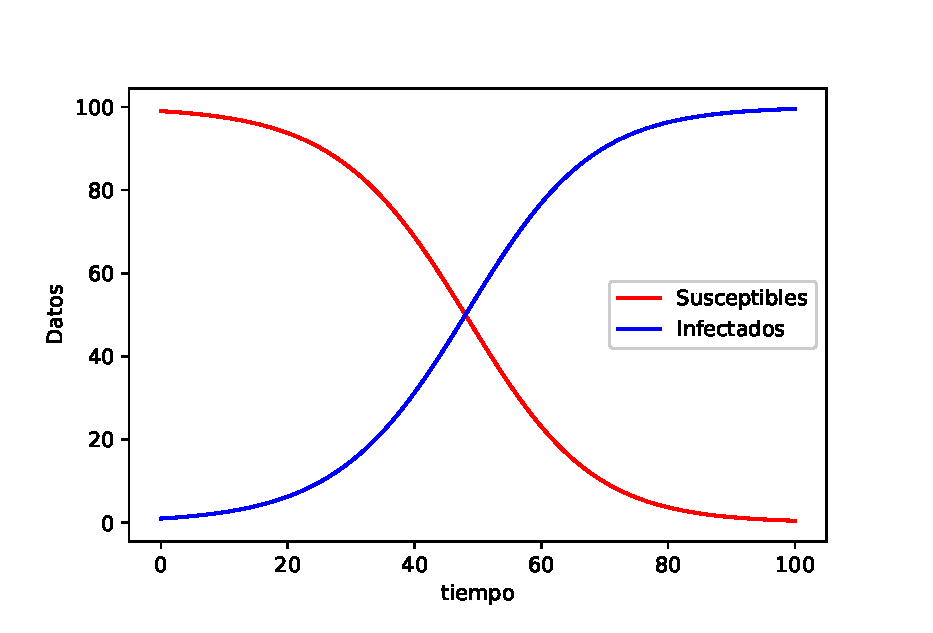
\includegraphics[scale=1]{graficaSI}
\end{center}
\end{figure}

En la figura \ref{fig: SI_IsobreS}, se representa el número de individuos infectados en función del númeor de susceptibles se aprecia una relación lineal pero inversamente proporcional, donde al subir el número de infectados baja el de susceptibles y al contrario.

\begin{figure}
\begin{center}
\caption{Gráfica del modelo SI, representando el número de infectados según el número de individuos susceptibles, en una población total de $100$ individuos, con valores iniciales $S_0=99, I_0 = 1, \alpha = 0.1, T_0 = 0, T = 100$.}
\label{fig: SI_IsobreS}
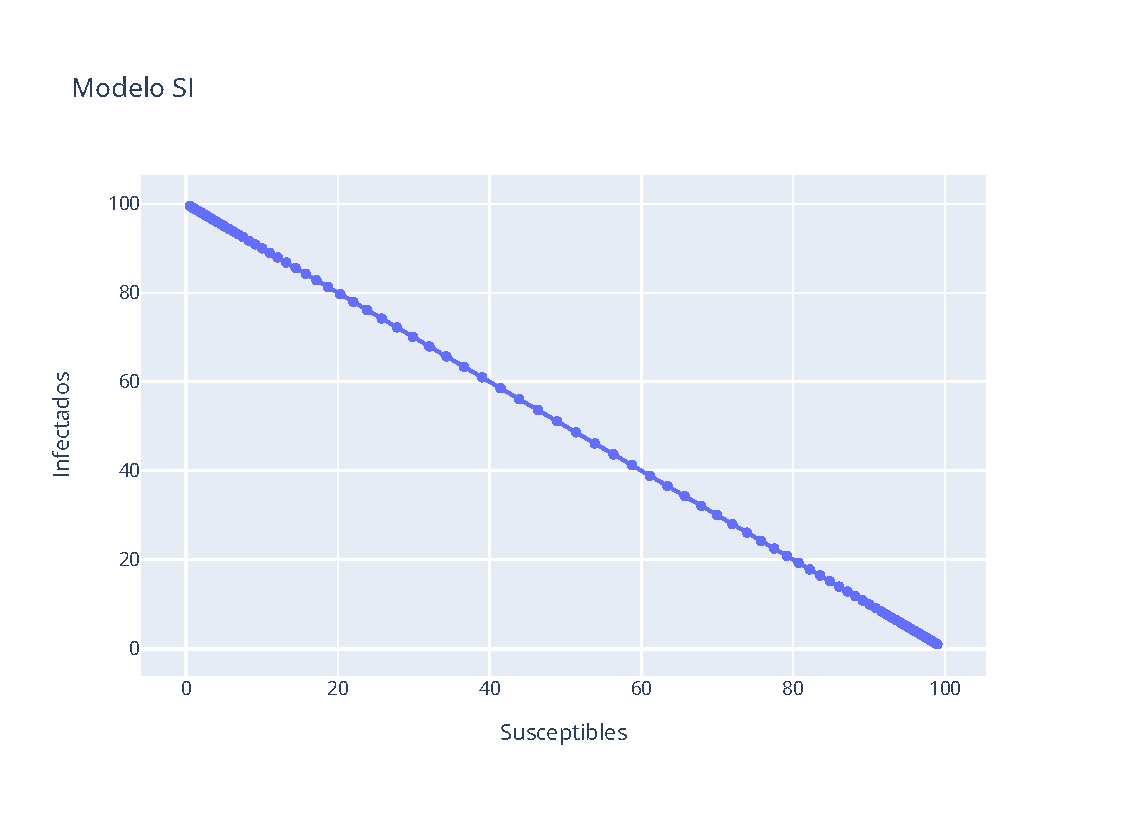
\includegraphics[scale=0.7]{SI_IsobreS}
\end{center}
\end{figure}

\section{Modelo SIR}
El modelo SIR comienza como el SI, pero tras infectarse los individuos pasan a un estado Recuperado, en el cual no pueden volver a infectarse ni infectar a otros.
Un ejemplo de este tipo de enfermedad es la varicela. 

El modelo es el siguiente:

\begin{equation}
\label{eqn: SIR_modelo}
\begin{aligned}
S_{n+1} = & S_n \left(1-\frac{\alpha\Delta t}{N} I_n \right) \\
I_{n+1} = & I_n \left( 1-\gamma \Delta t + \frac{\alpha\Delta t}{N} S_n \right) \\
R_{n+1} = & R_n + \gamma \Delta t I_n
\end{aligned}
\end{equation}

con condiciones iniciales $S_0>0$, $I_0>0$, $R_0\geq 0$, satisfaciendo $S_0+I_0+R_0=N$.

En estas ecuaciones, de nuevo tenemos que $\alpha$ es la tasa de contacto, esto es, el número medio de individuos con los que un infectado tiene suficiente contacto para contagiarlo en un intervalo de tiempo, y $\gamma$ es la probabilidad de que un infectado pase a recuperado/retirado/aislado/fallecido en un intervalo de tiempo, con $\alpha >0$ y $\gamma >0$.

Se supone que la población permanece constante, esto es: $S_n+I_n+R_n=N$.

\begin{proposition}
Las soluciones a este sistema discreto son positivas para cualquier valor de las condiciones iniciales si, y solo si:
$$\max{\big\{\gamma\Delta t, \alpha\Delta t\big\} } \leq 1$$

o equivalentemente:

$$\min{\bigg\{ \frac{1}{\gamma}, \frac{1}{\alpha} \bigg\} } \geq \Delta t$$

\end{proposition}

\begin{lemma}
$S_n$ es estrictamente decreciente y $R_n$ es estrictamentre creciente.
\end{lemma}

\begin{proof}

Sea $S_\infty=\lim_{n\rightarrow\infty} S_n\geq 0$, cuyo límite existe, pues es una sucesión estrictamente decreciente y acotada inferiormente por $0$.

Estudiamos las condiciones iniciales. Si $S_0\leq \frac{\gamma N}{\alpha}$, o, equivalentemente, $\mathcal{R}_{SIR}˘\leq 1$ entonces $I_1\leq I_0$ y, como $S_n$ es estrictamente decreciente, tenemos que $I_{n+1}\leq I_n$, es decir, no hay epidemia, ya que la velocidad de propagación no es lo bastante alta.

En otro caso, tenemos $S_0> \frac{\gamma N}{\alpha}$, entonces $I_1>I_0$. Debe ocurrir que $S_\infty <\frac{N\gamma}{\alpha}$, pues si no fuera así, tendríamos que $I_n$ crece hacia un equilibrio, $I_\infty$, lo que implica que $R_n$ se aproxima a infinito cuando $n\rightarrow\infty$, lo que no es posible, pues el total de la población es constante. Así, el número de infectados finalmente comienza a decrecer y se aproxima a $0$.
\end{proof}

\textcolor{red}{ el Lema 1 de \cite{allenDiscretetimeSISIR1994} dice que $S_\infty>0$. He estado mirando lo del lío con el límite de $S_n$, pero no he conseguido aclararme. Al hacerlo yo me sale que va a 0, pero el artículo original tiene este lema donde dice que el límite es mayor que 0 y no veo exactamente qué me estoy saltando en el razonamiento}

\begin{proof}
Comenzamos probando una de las implicaciones, suponiendo que $\max{\big\{\gamma\Delta t, \alpha\Delta t\big\} } \leq 1$.

Por hipótesis inicial, tenemos que $S_0, I_0, R_0>0$ y $S_0+I_0+R_0=N$, luego es suficiente comprobar que:
$$1-\frac{\alpha \Delta t}{N}I_0>0.$$
Lo cual es evidente, pues $\frac{I_n}{N}<1$ por hipótesis del modelo y $\alpha \Delta t<1$.

Por un razonamiento análogo, tenemos que $$1-\gamma \Delta t+\frac{\alpha\Delta t}{N}S_0 > 0.$$
Y finalmente $$R_0+\gamma\Delta t I_0>0$$ pues $\gamma>0$ y $\Delta t <0$.

Aplicando un razonamiento por inducción, suponiéndolo para $n$ se puede demostrar que $S_{n+1}, I_{n+1}, R_{n+1}$ son siempre positivas.

Para probar el recíproco basta probar que ambas cantidades son menores o iguales a $1$. Comenzamos trabajando en la primera ecuación \eqref{eqn: SIR_modelo}.
% suponemos la positividad para $n$ y probándola para $n+1$:

$$S_{n+1}=S_n\left(1-\frac{\alpha\Delta t}{N}I_n\right)$$
Por hipótesis $S_n>0$, entonces basta ver que $1-\frac{\alpha\Delta t}{N}I_n>0$. Usamos de nuevo que $I_n \leq N$ luego:
$$0<1-\frac{\alpha\Delta t}{N}I_n \leq 1-\alpha\Delta t,$$
y por tanto:
$$\alpha\Delta t  \leq 1.$$

En la segunda ecuación, como sabemos que $S_n$ es estrictamente decreciente, pues es una sucesión de la forma $S_{n+1}=\beta S_n$ con $\beta < 1$, entonces es cada vez más pequeño y el factor
$\frac{\alpha \Delta t}{N}S_n$ tiende a cero. \textcolor{red}{Aqui es donde uso que Sn tiende a 0, pero segun el articulo esto no es verdad}

Luego, despejando tenemos $\gamma\Delta t \leq 1$.

De la última ecuación no sacamos ninguna condición más, pues su solución es siempre positiva por definición de $\gamma$ y $\Delta t$.

\end{proof}

Por tanto, a partir del resultado anterior podemos deducir que el intervalo de tiempo, $\Delta t$, debe ser menor que el tiempo medio requerido para contagiar a oro individuo susceptible, $\alpha$, y menor que el período medio infeccioso, $\gamma$.
% Con contacto exitoso asumo que se refiere al tiempo necesario para infectar a un individuo. Sí es esto confirmado por la profe


El comportamiento global del sistema es fácil de ver. Definimos la tasa reproductiva como la constante 
$$\mathcal{R}_{SIR}=\frac{S_0 \alpha}{N\gamma }.$$

El valor de $\mathcal{R}_{SIR}$ determina el comportamiento global del modelo.

En otros trabajos como \cite{demongeotSIEpidemicModel} esta tasa reproductiva se llama tasa de transmisión media.

Además, sabemos por el Lema 1 de \cite{allenDiscretetimeSISIR1994} que $S_\infty>0$.
El modelo continuo correspondiente al modelo SIR se comporta de la misma forma que el modelo discreto, y viene expresado por:

\begin{equation}
\label{eqn: modelo_SIR_continuo}
\begin{aligned}
S'(t) = & -\dfrac{\alpha}{N}SI \\
I'(t) = & I\left(\dfrac{\alpha}{N}S-\gamma \right) \\
R'(t) = & R+\gamma I
\end{aligned}
\end{equation}

donde $S(0)+I(0)+R(0)=N$. La tasa reproductiva en este caso se define como
$$\mathcal{R}_{SIR}=\frac{S(0)\alpha }{N\gamma },$$
y si como hemos visto $\mathcal{R}_{SIR}\leq 1$  se dice que no hay epidemia, pero en cambio, si es mayor, se dice que sí la hay.

\begin{figure}
\begin{center}
\caption{Gráfica del modelo SIR, en una población total de $100$ individuos, con valores iniciales $S_0=99, I_0 = 1, R_0 = 0, \alpha = 0.1, \gamma = 0.01 T_0 = 0, T = 300$.}
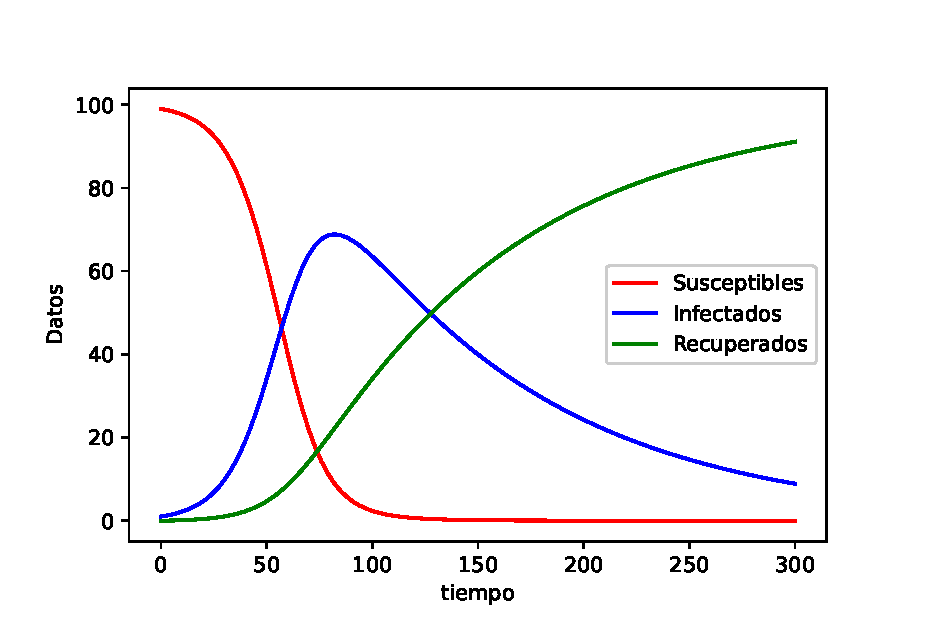
\includegraphics[scale=1]{graficaSIR}
\end{center}
\end{figure}

En la figura \ref{fig: SIR_IsobreS} se representan el número de infectados en función de los individuos susceptibles. En este modelo, al contrario de lo que ocurría en el modelo SI no son inversamente proporcionales. Vemos que primero los infectados crecen al descender el número de individuos susceptibles, esto es porque las personas susceptibles se infectan, pero después aunque los individuos susceptibles sigan disminuyendo los infectados bajan, esto es debido a que los individuos previamente infectados se están recuperando.

\begin{figure}
\begin{center}
\caption{Gráfica del modelo SI, representando el número de infectados según el número de individuos susceptibles, en una población total de $100$ individuos, con valores iniciales $S_0=99, I_0 = 1, \alpha = 0.1, \gamma=0.01, T_0 = 0, T = 300$.}
\label{fig: SIR_IsobreS}
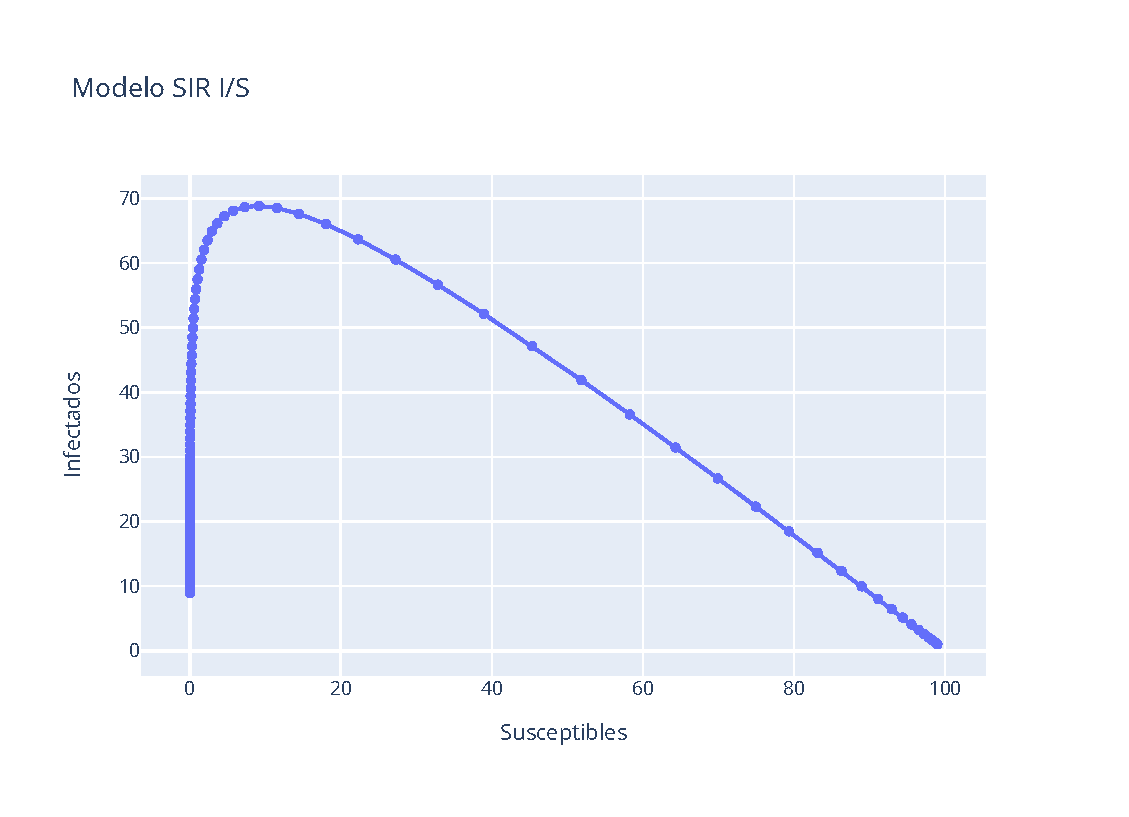
\includegraphics[scale=0.7]{SIR_IsobreS}
\end{center}
\end{figure}

Estudiamos ahora la figura \ref{fig: SIR_RsobreS}, en la que se muestra como varían los individuos recuperados en función de los susceptibles.

A medida que los individuos susceptibles decrecen los recuperados aumentan, pero no lo hacen de forma lineal. Esto se debe a que los individuos susceptibles primero deben infectarse y luego recuperarse, y, como ya hemos visto en la figura \ref{fig: SIR_IsobreS} los infectados bajan muy rápidamente cuando las personas susceptibles son pocas, por ello los recuperados también crecen rápidamente a menor número de individuos susceptibles.

\begin{figure}
\begin{center}
\caption{Gráfica del modelo SIR discreto, representando el número de recuperados según el número de individuos susceptibles, en una población total de $100$ individuos, con valores iniciales $S_0=99, I_0 = 1, \alpha = 0.1, \gamma=0.01, T_0 = 0, T = 300$.}
\label{fig: SIR_RsobreS}
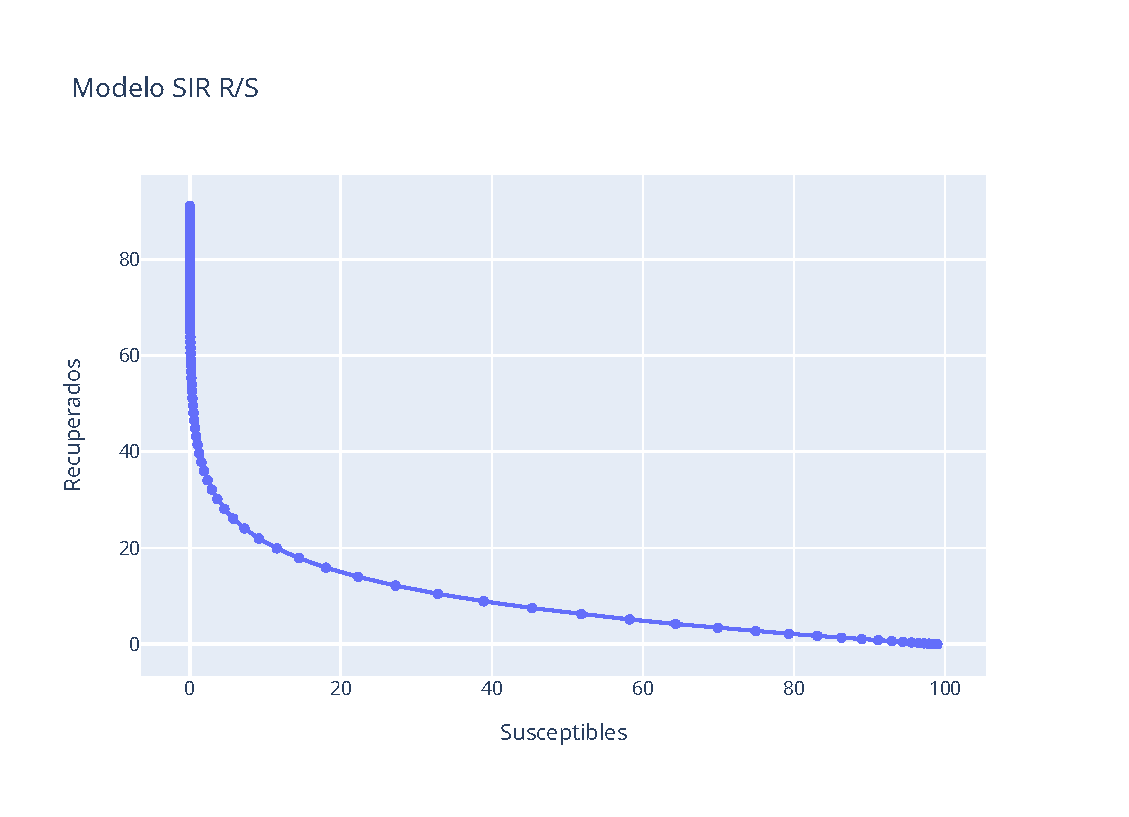
\includegraphics[scale=0.7]{SIR_RsobreS}
\end{center}
\end{figure}

Finalmente, en la figura \ref{fig: SIR_RsobreI} se muestran los individuos recuperados en función de los infectados.

Cabe destacar que para cada valor de los infectados hay dos valores de recuperados, esto se debe a que al comienzo, cuando los infectados están creciendo hay pocos recuperados, después los recuperados aumentan y los infectados decrecen. Es decir, para cada valor de infectados hay dos de recuperados, el primero cuando los infectados están creciendo y hay pocos recuperados y después cuando los infectados decrecen y hay muchos recuperados . Otra cosa a tener en cuenta es la distancia entre las marcas en la curva. Cada marca indica la medida del número de infectados y recuperados en un mismo tiempo $t$.

Al comenzar el número de recuperados es bajo y crece despacio a medida que aumentan los infectados. Llega un punto máximo del número de infectados, en el que se produce la curva, y cuando los infectados comienzan a descrecer los recuperados aumentan rápidamente, lo que se puede ver por la distancia más corta que hay entre las marcas de la curva.

\begin{figure}
\begin{center}

\caption{Gráfica del modelo SI discreto, representando el número de recuperados según el número de individuos infectados, en una población total de $100$ individuos, con valores iniciales $S_0=99, I_0 = 1, \alpha = 0.1, \gamma=0.01, T_0 = 0, T = 300$.}
\label{fig: SIR_RsobreI}
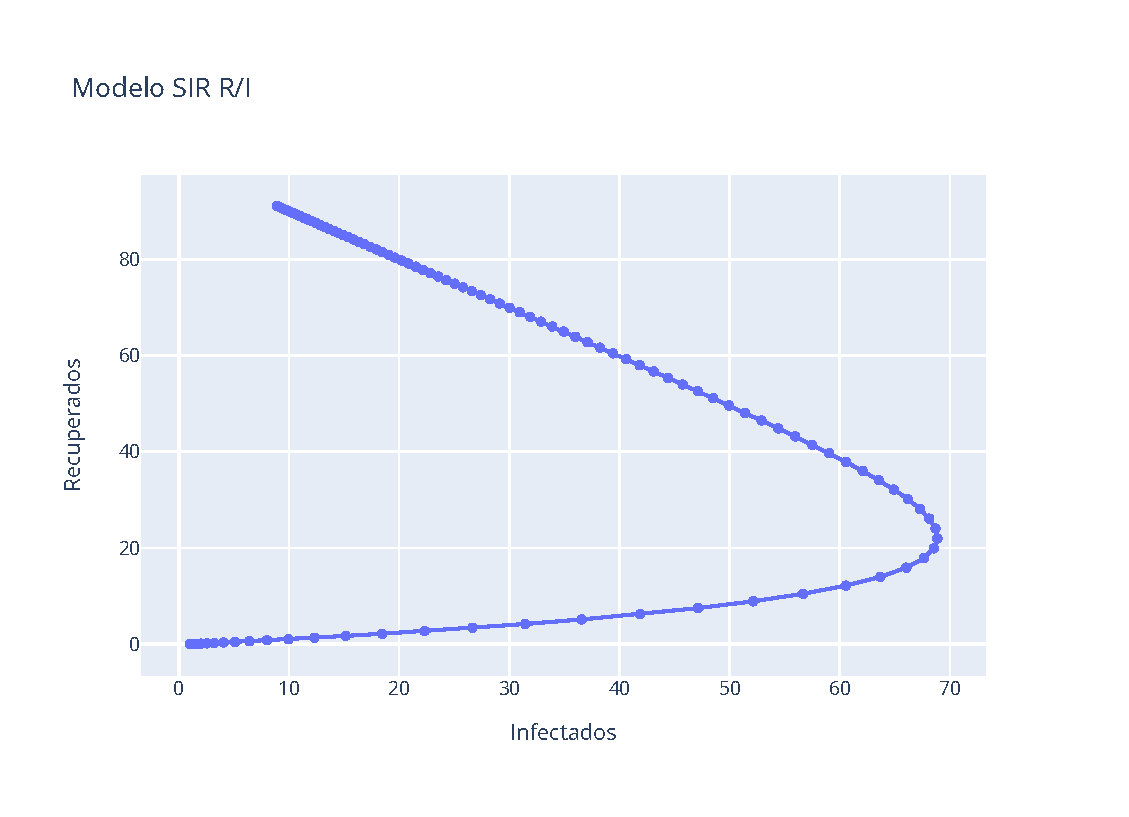
\includegraphics[scale=0.7]{SIR_RsobreI}
\end{center}
\end{figure}


\section{Modelo SIS}
El modelo SIS es similar al SI, con la salvedad de que los individuos son susceptibles de múltiples reinfecciones.
Por ejemplo, los resfriados pueden modelarse usando SIS.

El modelo es una perturbación del modelo SI descrito anteriormente. Se define de la siguiente forma:

\begin{equation}
\label{eqn: modelo_SIS}
\begin{aligned}
S_{n+1} = S_n \left(1-\frac{\alpha\Delta t}{N} I_n \right) + \gamma \Delta t I_n \\
I_{n+1} = I_n \left( 1-\gamma \Delta t + \frac{\alpha\Delta t}{N} S_n \right)
\end{aligned}
\end{equation}

con condiciones iniciales positivas $S_0>0$, $I_0>0$ cumpliendo $S_0+I_0=N$. Por lo tanto, el tamaño de la población es constante.

En estas ecuaciones, $\alpha$ de nuevo representa la tasa de contacto, esto es, el número medio de individuos con los que un infectado tiene suficiente contacto para contagiarlo en un intervalo de tiempo, y $\gamma$ es la probabilidad de que un infectado pase a recuperado/retirado/aislado/fallecido en un intervalo de tiempo, donde se cumple $\alpha >0$ y $\gamma >0$.

\begin{proposition}
Las soluciones de \eqref{eqn: modelo_SIS} siempre son positivas si, y solo si:

$$\gamma \Delta t \leq 1 $$ y $$\alpha\Delta t< \left( 1+\sqrt{\gamma \Delta t} \right)^2$$

\end{proposition}
\begin{proof}
Sea $I_0=\epsilon$ y $S_0=N-\epsilon$, entonces por la definición del modelo tenemos:
\begin{equation}
\begin{aligned}
I_1 & =\epsilon\left(1-\gamma\Delta t+\alpha\Delta t\frac{N-\epsilon}{N}\right) \\
& = -\frac{\alpha\Delta t \epsilon^2}{N} + \epsilon(1-\gamma\Delta t+\alpha\Delta t ) \\
& = p(\epsilon) \\
\end{aligned}
\end{equation}

Luego tenemos que ver cuándo la parábola satisface $0<p(\epsilon)<N$ para $0<\epsilon<N$.

Notemos que $p(0)=0$ y $p(N)=N(1-\gamma\Delta t).$

Sea $(\epsilon^*, p^*)$ el vértice de la parábola, entonces 
$$(\epsilon^*, p^*) = \left(\frac{N(1-\gamma\Delta t+\alpha\Delta t)}{2\alpha\Delta t}, \frac{N(1-\gamma\Delta t+\alpha\Delta t)^2}{4\alpha\Delta t}\right)$$

Por tanto, $0<p(\epsilon )<N$ para $0<\epsilon <N$ si y solo si:

$$\gamma\Delta t \leq 1,$$

y por tanto, o bien $\epsilon^* \geq N$, que es equivalente a $\alpha\Delta t \leq 1-\gamma\Delta t$. bien $\epsilon^*<N \text{  y  } p^*<N$, lo que requiere que $\alpha\Delta t > 1-\gamma\Delta t$ y $(1-\gamma\Delta t+\alpha\Delta t)^2<4\alpha\Delta t$. Estas desigualdades se dan si y solo si:

$$1-\gamma\Delta t < \alpha \Delta t < \left( 1+\sqrt{\gamma \Delta t} \right)^2.$$

\end{proof}

En el modelo SIS, la tasa reproductiva se define como 
$$\mathcal{R}_{SIS}=\frac{\alpha}{\gamma}.$$


\begin{lemma}
Si $\mathcal{R}_{SIS}\leq 1$ entonces se tiene que $I_{n+1} < I_n$, ya que $0<S_n<N$ y las soluciones son positivas. En este caso es fácil ver que el límite, al ser una sucesión monótona decreciente y acotada inferiormente, es $(S^*,I^*)=(N,0)$.

Si $\mathcal{R}_{SIS}>1$ las soluciones convergen si se cumple la condición$\alpha \Delta t \leq 2+\gamma \Delta t$
\end{lemma}

\begin{proof}
Supongamos que $S^*<N$, entonces existen $n_1, \epsilon$ tales que para todo $n \geq n_1$:
$$S_n<S^*+\epsilon < N$$
y usando las ecuaciones \eqref{eqn: modelo_SIS}
\begin{equation}
\begin{aligned}
I_{n+1}  & \leq I_n \left( 1-\gamma \Delta t + \frac{\alpha\Delta t}{N} S_n \right) \\
& \leq I_n \left( 1-\gamma \Delta t + \alpha\Delta t \right)
& \leq I_n \rho 
\end{aligned}
\end{equation}


donde hemos denotado $\rho = 1-\gamma \Delta t + \alpha\Delta t$.

Como $\rho < 1$ tendríamos que $I^*=0$, lo que contradice que $S^*<N$.

Si $\mathcal{R}_{SIS}>1$ realizando la sustitución $S_n=N-I_n$ y el cambio

$$x_n=\frac{\alpha \Delta t I_n}{N(1+\alpha \Delta t - \gamma \Delta t)}$$

tenemos:

\begin{equation}
\begin{aligned}
\alpha\Delta t I_n = x_nN(1+\alpha\Delta t-\gamma\Delta t) \Leftrightarrow \\
I_n = x_n\frac{N(1+\alpha\Delta t - \gamma\Delta t)}{\alpha\Delta t}
\end{aligned}
\end{equation}

entonces sustituyendo en la ecuación \eqref{eqn: modelo_SIS}:

\begin{equation}
\begin{aligned}
x_{n+1}\frac{N(1-\alpha\Delta t-\gamma\Delta t)}{\alpha \Delta t} = x_n\frac{N(1+\alpha\Delta t-\gamma \Delta t)}{\alpha\Delta t}\left( 1-\gamma\Delta t+\frac{\alpha\Delta t}{N}\left(N-x_n\frac{N(1+\alpha\Delta t-\gamma\Delta t)}{\alpha\Delta t}\right) \right)
\end{aligned}
\end{equation}

Despejando de esta expresión:

\begin{equation}
\begin{aligned}
x_{n+1} & = x_n\left( 1-\gamma\Delta t+\frac{\alpha\Delta t}{N}N-\frac{\alpha\Delta t}{N}x_n\frac{N(1+\alpha\Delta t -\gamma \Delta t)}{\alpha\Delta t} \right) \\
& = x_n(1-\gamma\Delta t + \alpha\Delta t -x_n(1+\alpha\Delta t -\gamma\Delta t)) \\
& = x_n((1-\gamma\Delta t+\alpha\Delta t)(1-x_n))
\end{aligned}
\end{equation}

luego obtenemos la ecuación logística con parámetro $\mu = 1+\alpha\Delta t -\gamma \Delta t$

$$x_{n+1} = (1+\alpha \Delta t - \gamma \Delta t)x_n(1-x_n).$$

En el modelo SIS la restricción necesaria para garantizar soluciones positivas no es suficiente para asegurar la convergencia. En este caso a dicha restricción hay que añadir la condición $\alpha \Delta t \leq 2+\gamma \Delta t$, restricción del parámetro de la ecuación logística para la convergencia.

\end{proof}


\begin{figure}
\begin{center}
\caption{Gráfica del modelo SIS, en una población total de $100$ individuos, con valores iniciales $S_0=95, I_0 = 5, \alpha = 0.1, \gamma=0.01, T_0 = 0, T = 150$.}
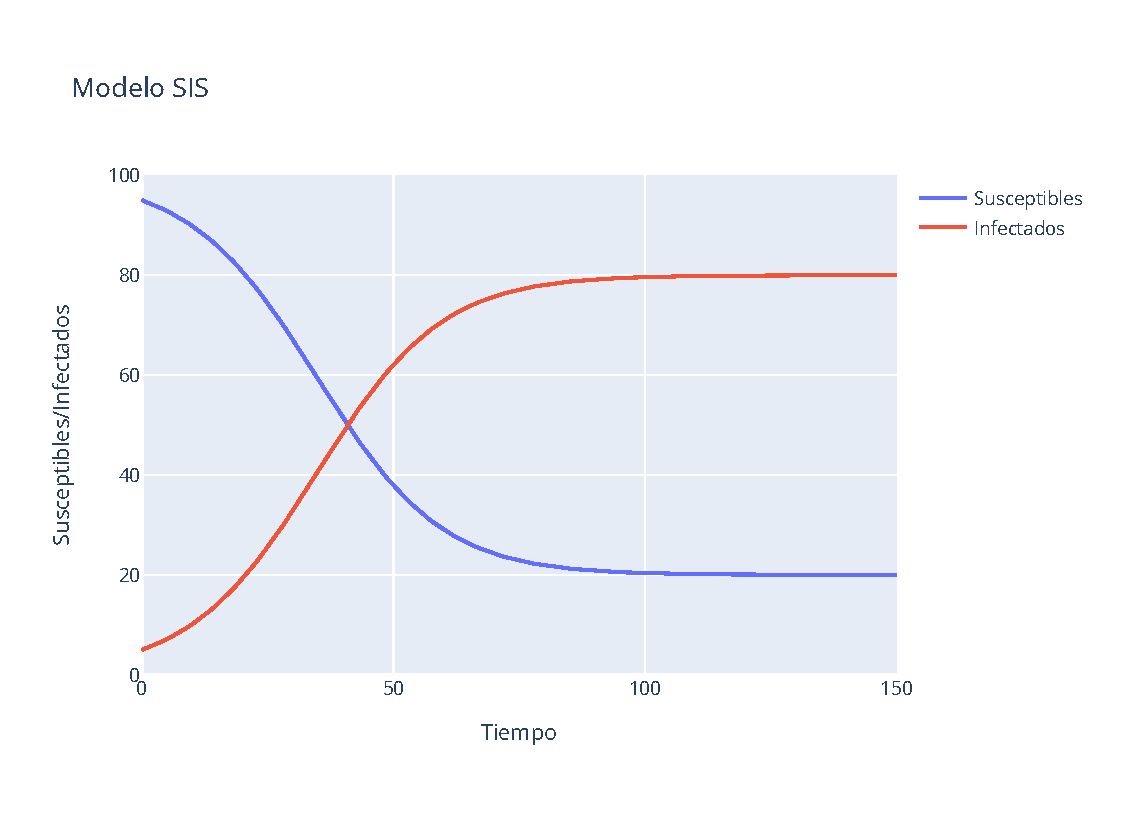
\includegraphics[scale=0.7]{SIS_modelo}
\end{center}
\end{figure}

En la figura \eqref{fig: SIS_IsobreS} se representa el número de infectados en función del número de individuos susceptibles. Se puede ver que son inversamente proporcionales, es decir, a mayor número de infectados menos individuos susceptibles hay y al revés.

Cabe destacar el parecido de esta gráfica con su análoga del modelo SI \eqref{fig: SI_IsobreS}.

\begin{figure}
\begin{center}
\caption{Gráfica del modelo SIS discreto, representando el número de infectados según el número de individuos susceptibles, en una población total de $100$ individuos, con valores iniciales $S_0=95, I_0 = 5, \alpha = 0.1, \gamma=0.01, T_0 = 0, T = 200$.}
\label{fig: SIS_IsobreS}
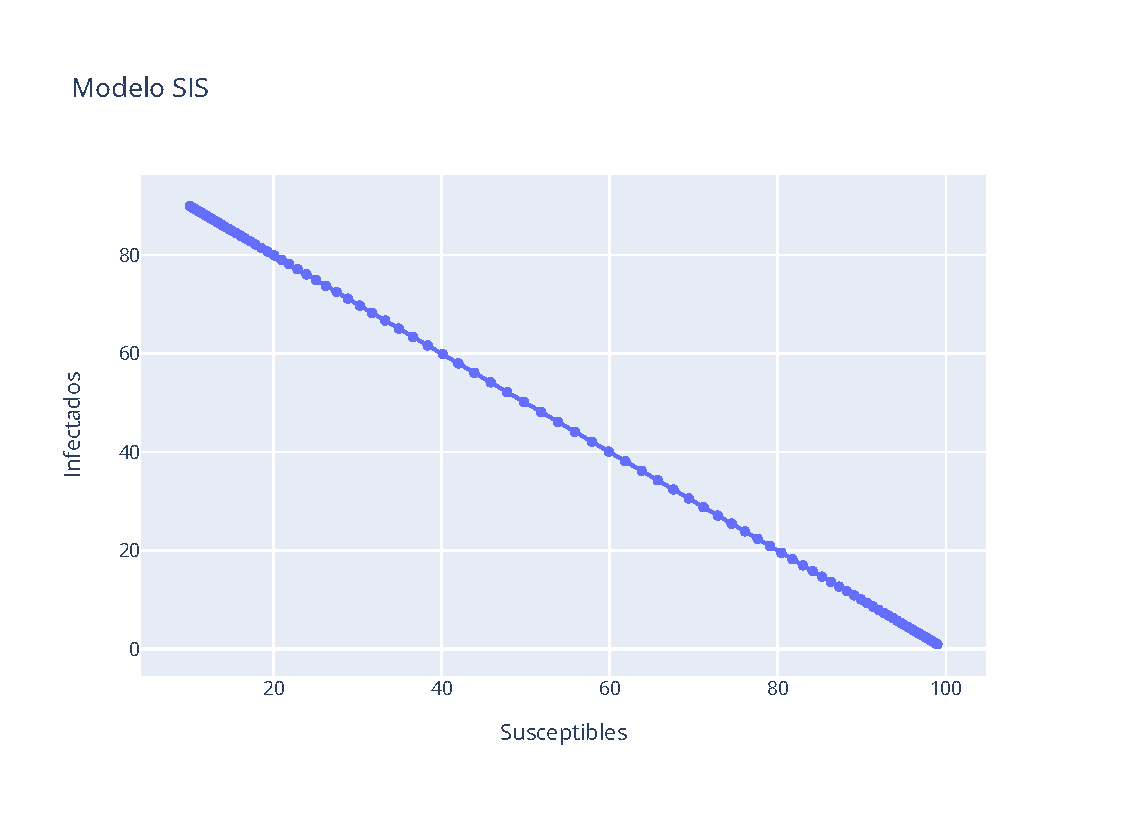
\includegraphics[scale=0.7]{SIS_IsobreS}
\end{center}
\end{figure}







\section{Análisis de los parámetros de los modelos}

\subsection{Introducción}

Estimar la tasa de transmisión media es uno de los aspectos más cruciales en epidemiología. Esta tasa condiciona la fase de la epidemia e incluso si va a extinguirse. Es combinación de tres factores:

\begin{enumerate}
\item Coeficiente de virulencia: Relacionado con el agente infeccioso.
\item Coeficiente de susceptibilidad: Relacionado con el anfitrión.
\item Número de contactos por unidad de tiempo entre individuos.
\end{enumerate}

Los dos primeros factores se tienen en cuenta a la vez en la probabilidad de transmisión.

Todos los factores pueden cambiar con el tiempo. El primero, debido a mutaciones del virus y los dos últimos por medidas de contención. Por tanto, observar el decrecimiento de la transmisión media en una enfermedad es una buena forma de comprobar la efectividad de las medidas de contención.

En el artículo \cite{demongeotSIEpidemicModel} se presenta un modelo SI modificado con el objetivo de compararlo con los datos obtenidos en la pandemia de la COVID-19 hasta el momento, y así tratar de predecir su comportamiento en el futuro.

El modelo SI continuo considerado es el siguiente:

\begin{equation}
\label{eqn: SI_cont}
\begin{aligned}
S'(t) = & -\tau (t)S(t)I(t) \\
I'(t) = & \tau (t)S(t)I(t) -vI(t)
\end{aligned}
\end{equation}

donde $S(t)$ es el número de individuos susceptibles , $I(t)$ el número de individuos infectados en el tiempo $t$ y $\tau (t)$ la tasa de transmisión, que combina el número de contactos por unidad de tiempo y la probabilidad de transmisión. Observemos que $\tau (t)$ se considera variable respecto al tiempo, al contrario que en el caso SI clásico estudiado antes. Además, notemos que $v$ es una constante, donde $1/v$ es la duración media del período de infección, y $vI(t)$ el flujo de individuos recuperados o fallecidos. %vI(t) es el flujo de recuperados o muertos porque ha mezclado el modelo SI y SIR; vI(t) serian los recuperados, pero se ahorra la ecuacion de la R

Se consideran las condiciones iniciales

$$S(t_0)=S_0>0, \: I(t_0)=I_0>0.$$

Ahora, consideramos que al final del período infeccioso nos han informado de una fracción del total de casos, en este caso la fracción la denotamos por $f\in (0,1]$. Sea $C_R(t)$ el número total acumulado de casos reportados. Entonces:

\begin{equation}
\label{eqn: acumulada}
C_R(t) = {C_R}_0 + vfC_I(t) \; \forall t \geq t_0
\end{equation}

donde $C_{R0}$ representa el número de casos reportados al inicio del estudio y 

$$C_I(t) = \int_{t_0}^t I(w) dw $$

siendo $C_I$ el número total de infectados acumulado.

Asumimos conocidos $S_0 > 0$, $1/v>0$, $f\in (0,1]$. Por tanto, queremos averiguar el número inicial de infectados $I_0$ y la tasa de transmisión $\tau (t)$.

\subsection{Aproximación de $I_0$ y $\tau (t_0)$}
Procedemos a intentar aproximar $I_0$ y $\tau (t_0)$:

Al comienzo de la pandemia podemos suponer que $S(t)$ y $\tau (t)$ son constantes e iguales a $S_0$ y $\tau_0 = \tau (t_0)$, respectivamente. Sustituyendo estos valores en la ecuación \eqref{eqn: SI_cont} obtenemos:

$$I'(t) = (\tau_0 S_0 -v) I(t).$$

Resolviendo la ecuación diferencial llegamos a:

$$I(t) = I_0\exp{((\tau_0 S_0-v)(t-t_0))}.$$

Sustituyendo en \eqref{eqn: acumulada}:

$$C_R(t) = {C_R}_0 + vfI_0\frac{\mathrm{e}^{(\tau_0 S_0 -v)(t-t_0)} -1}{\tau_0 S_0-v}.$$

De este modo, hemos obtenido un primer modelo para los casos acumulados al principio de la pandemia.

Reescribimos la ecuación anterior como:

\begin{equation}
\label{eqn: acumulada_modelo}
C_R(t) = \chi_1 \mathrm{e}^{\chi_2 t} -\chi_3.
\end{equation}

Estimamos $\chi_3$ usando los datos de la epidemia obtenidos, y el mejor ajuste para los datos se obtiene con $\chi_3=0$.

Ahora, usando \eqref{eqn: acumulada} y \eqref{eqn: acumulada_modelo} tenemos:

\begin{equation}
I_0=\frac{\chi_1\chi_2\mathrm{e}^{\chi_2 t_0}}{vf}
\end{equation}

Y, como sabemos que $\chi_2 = \tau_0 S_0-v$, entonces

\begin{equation}
\tau_0 = \frac{\chi_2+v}{S_0}.
\end{equation}

Si suponemos $\tau (t) = \tau_0$ constante, tenemos que el modelo queda:

\begin{equation}
\begin{aligned}
S'(t) = -\tau_0S(t)I(t) \\
I'(t) = \tau_0S(t)I(t) -vI(t)
\end{aligned}
\end{equation}

Usando la ecuación de $S(t)$ y resolviéndola obtenemos:

$$S(t) = S_0\exp{\left( -\tau_0 \int_{t_0}^t I(w) dw \right)} = S_0\exp{(-\tau_0 C_I(t))}$$

Ahora, sustituyendo esta expresión en la ecuación de $I(t)$ del modelo y usando $C_I'(t)=I(t)$:

$$I'(t) = S_0\exp{\left( -\tau_0 C_I(t)\right) }\tau_0 C_I'(t)-vI(t)$$

Finalmente, integrando entre $t_0$ y $t$ tenemos que:

$$I(t)=C_I'(t)=I_0+S_0(1-\exp{(-\tau_0 C_I(t)}))-vC_I(t)$$
 
Observamos entonces que el número total de infectados es monótono creciente, ya que $I(t)>0$ siempre por positividad de las soluciones y $C_I'(t)=I(t)>0$. Cabe destacar que esto no implica que el número de infectados sea monótono creciente.

\begin{theorem}
Sea $t>t_0$ fijo. El número de infectados acumulados es estrictamente creciente respecto a las siguiente cantidades:
\begin{itemize}
\item $I_0>0$: Número inicial de infectados
\item $S_0>0$: Número inicial de individuos susceptibles.
\item $\tau>0$: Tasa de transmisión
\item $1/v$: Tiempo medio de la infección.
\end{itemize}
\end{theorem}

\subsection{Fórmula teórica para $\tau (t)$}

Usando la ecuación del modelo inicial \eqref{eqn: SI_cont} obtenemos:
% La ecuacion de la S$

$$S(t) = S_0 \exp{\left( - \int_{t_0}^t \tau(w) I(w) dw \right) } $$ 

Ahora, sustituyendo en la ecuación \eqref{eqn: SI_cont}:
% La ecuacion de la I

$$I'(t) = S_0 \exp{\left( - \int_{t_0}^t \tau(w) I(w) dw \right) } \tau (t) I(t) -vI(t) $$

Integramos en ambos lados entre $t_0$ y $t$, luego:

$$ C_I'(t) = I_0 + S_0 \left( 1-\exp{\left(- \int_{t_0}^t \tau (w) I(w)dw \right)}\right) -vC_I(t)$$

Equivalentemente, por \eqref{eqn: acumulada}:

$$C_R'(t) = vf\left( I_0 + S_0 \left( 1-\exp{\left(- \frac{1}{vf}\int_{t_0}^t \tau (w ) I(w)dw \right)}\right)\right) +v{C_R}_0 -vC_R(t)$$

\textcolor{red}{TODO Esta cuenta no termina de salirme, pero tiene más o menos sentido}

Así, obtenemos el Teorema 3.1 de \cite{demongeotSIEpidemicModel}, que nos da la relación directa buscada.

\textcolor{blue}{He estado leyendo el resto del artículo, en el que habla de obtener una expresión explícita de $\tau (t)$ e $I_0$, pero para eso usan datos de China en específico y ajustes por ordenador, así que no tengo muy claro si merece la pena incluir esa parte ya que no tenemos los datos y por tanto sería fiarse un poco de lo que han hecho ellos}










% Part II
%\input{chapters/chapter5}

% ----------------------- %
% BIBLIOGRAFÍA
% ----------------------- %

% Estilo de cita.
%\usepackage{natbib} YA SE IMPORTA EN OTRO PUNTO, NO HACE FALTA PONERLO AQUI
% FUENTE CUSTOM
%\bibliographystyle{apa-good}
% formato de citas original
\bibliographystyle{unsrtnat}

%[citestyle=numeric]

% Añadimos la bibliografía al índice
%\phantomsection
%\addcontentsline{toc}{chapter}{Bibliografía}

\chapter{Contenido adicional}
\section{Ejecución de código}
Para la ejecución de código se ha usado Google Colab usando un cuaderno en línea con python. Por ello, la estructura del fichero de código consta de algunas celdas para cargar el google drive o usar una estructura de carpetas que no va incorporada en la práctica, de cara a comprobar si el código funciona.

Se recomienda la ejecución del código usando google colab en caso de que fuera necesario. La base de datos debe encontrarse subida a drive y en content las carpetas de cada caso con una subcarpeta por algoritmo, teniendo en cuenta que el caso 2 está dividido en dos subcasos, llamados caso2A y caso2B.

Así, en el primer nivel de carpetas tendríamos caso1, caso2A, caso2B y caso3. Y dentro de cada una de ellas una carpeta por algoritmo, llamadas como sigue: kmeans, birch, dbscan, spectral y meanshift.

Además, hay varios scripts para sacar gráficas auxiliares (los gráficos de barras de los tamaños de los clusters y las gráficas de los estudios de parámetros) que se encuentran en ficheros.py y no en el cuaderno.

Como comentario final, para generar unas gráficas u otras se debe comentar o descomentar la sección correspondiente a las gráficas en el código.

\section{Gráficas}
En la memoria se han incluido solamente las gráficas que se han considerado relevantes, pero se pueden encontrar más gráficas dentro de la carpeta figures o graficas, donde también hay varios scripts para generarlas.


\chapter{Bibliografía}
\begin{itemize}
\item Diapositivas de la asignatura.
\item \href{http://scikit-learn.org/stable/modules/clustering.html}{http://scikit-learn.org/stable/modules/clustering.html}
\item \href{http://www.learndatasci.com/k-means-clustering-algorithms-python-intro/}{http://www.learndatasci.com/k-means-clustering-algorithms-python-intro/}
\item \href{https://pandas.pydata.org/docs/}{https://pandas.pydata.org/docs/}
\item \href{https://seaborn.pydata.org/introduction.html}{https://seaborn.pydata.org/introduction.html}
\item \href{https://matplotlib.org/}{https://matplotlib.org/}
\end{itemize}

%\bibliography{bib/library}

\end{document}